\documentclass[10pt]{article}
\usepackage[utf8]{inputenc}

% packages for math
\usepackage{amssymb, amsthm, amsmath, geometry, esint, mathrsfs, mathtools}
% \usepackage{MnSymbol}
% packages for figures
\usepackage{graphicx, float, caption, subcaption}
% other packages I always use
\usepackage{cancel, bm, verbatim, fancyvrb, url, enumitem}
% package for strikethrough
% \usepackage{ulem} % This makes \emph do underlining, rather than italics.
% package for "strikeout goes to zero"
\usepackage{cancel}
% packages for headings
\usepackage{fancyhdr}
% Write pseudocode
% \usepackage[ruled, vlined]{algorithm2e}
% \usepackage{algorithm}
% \usepackage{algpseudocode}

% [https://www.overleaf.com/learn/latex/Code_Highlighting_with_minted]
\usepackage{minted, listings}
\usemintedstyle{perldoc}

% line spacing
\renewcommand{\baselinestretch}{1.1}
% control all four margins
\newgeometry{left=0.5in, right=0.5in, top=1.0in, bottom=1.0in}

% More control aligning figures
\usepackage[export]{adjustbox}

% Enable svg
\usepackage{svg}

% control section heading sizes
\usepackage{titlesec}
\titleformat{\section}
    {\normalfont\fontsize{14}{14}\bfseries}{\thesection}{1em}{}
\titleformat{\subsection}
    {\normalfont\fontsize{13}{13}\bfseries}{\thesubsection}{1em}{}
\titleformat{\subsubsection}
    {\normalfont\fontsize{12}{12}\bfseries}{\thesubsubsection}{1em}{}
    
% hyperlink appearance settings
\usepackage{hyperref}
\hypersetup{
    colorlinks=true,
    linkcolor=blue,
    filecolor=magenta,
    urlcolor=blue
}
\urlstyle{same}

% settings for "itemize" environment
\setlist{noitemsep}
\renewcommand\labelitemi{$\rightarrow$}

% Enable paragraphs inside itemize/enumerate environments.
\setlist{
  listparindent=\parindent,
  parsep=0pt,
}

%\setlength{\parindent}{0cm}

% headers
\pagestyle{fancy}
\fancyhf{}
\rhead{}
\chead{}
\lhead{}
\cfoot{\thepage}

% For displaying keyboard commands, etc.
\usepackage[utf8]{inputenc}
\usepackage[os=mac, mackeys=symbols]{menukeys}
% %Windows
% \usepackage[os=win]{menukeys}
% %Mac OS X (symbols)
% \usepackage[os=mac, mackeys=symbols]{menukeys}
% %Mac OS X (text)
% \usepackage[os=mac, mackeys=text]{menukeys}

% Enable pointy individual menu items. Hack from [https://tex.stackexchange.com/a/515436].
\makeatletter
\tikzset{menu hack/.cd,
t>/.code={\tikzset{tw@menus@base/.append style={signal to=east}}},
>t/.code={\tikzset{tw@menus@base/.append style={signal from=west}}}}
\newcommand{\Menu}[2][]{\begingroup%
\tikzset{menu hack/.cd,#1}%
\menu{#2}%
\endgroup}
\makeatother

% Define how names of Blender objects are rendered.
\newcommand{\obj}[1]{\menu{\color{magenta} #1}}

% Render pictures (usually icons) inline. Hack from [https://tex.stackexchange.com/a/139150].
\DeclareRobustCommand{\inlinepic}[1]{%
  \begingroup\normalfont
  % \includegraphics[height=\fontcharht\font`\B]{#1}%
  \includegraphics[height=1.5em, valign=c]{#1}%
  \endgroup
}

% defining my own math shortcuts
\newcommand{\R}{\mathbb{R}}
\newcommand{\Z}{\mathbb{Z}}
\newcommand{\C}{\mathbb{C}}
\newcommand{\Q}{\mathbb{Q}}
\newcommand{\p}{\partial}
\newcommand{\bb}{{\bf b}}
\newcommand{\bu}{{\bf u}}
\newcommand{\bv}{{\bf v}}
\newcommand{\bw}{{\bf w}}
\newcommand{\bx}{{\bf x}}
\newcommand{\bomega}{\bf \omega}
\newcommand{\bE}{\bf E}
\DeclareMathOperator{\Real}{Re}
\DeclareMathOperator{\Imag}{Im}
\DeclareMathOperator{\Log}{Log}
\DeclareMathOperator{\Arg}{Arg}
\DeclareMathOperator{\Abs}{Abs}
\DeclareMathOperator{\divr}{div}
\DeclareMathOperator{\tr}{tr}
\DeclareMathOperator{\argmin}{argmin}

% Get SVG Blender icons from this repo: [https://github.com/Shrinks99/blender-icons]
% Navigate more easily at this website: [https://wilkinson.graphics/blender-icons/]

\begin{document}

{\bf Last updated:} \today

\tableofcontents

\newpage

\section*{Introduction}

\subsection{Software/hardware versions used in this document --- warning!}
\begin{itemize}
    \item Blender examples were generated using at least Blender version 3.0.0.
    \item In versions 3.4 and beyond, the function of the \obj{Transfer Attribute} geometry node has been incorporated into the \obj{Sample Index} node instead. Many of my examples here still reference the \obj{Transfer Attribute} node, but be warned that a node by this name no longer exists in the most recent version of Blender!
    \item There will be some difference between Mac and PC commands. The main difference vs. Mac is that \keys{\ctrl} becomes \keys{\cmd} (command) on Mac. I'm not sure what else changes. Maybe some keyboard shortcuts that involve keys like \keys{Alt}. Throughout the document I try to describe both types of keyboard commands.
\end{itemize}

\subsection{Notation}
\begin{itemize}
    \item References to Blender objects, nodes, etc. are rendered as such: \obj{Curve}, \obj{Camera}, etc.
    \item Menu options that are navigated to primarily using tabs are rendered as such: \menu{Properties > Object Properties}. I try to use this notation to indicate pages within ``main'' menus, i.e. the menus that are readily visible on the top and sides of the Blender window. Single tabs are still rendered point-ily: \Menu[t>]{Properties}, \Menu[t>]{Object}, etc.
    \item I try to indicate secondary menu or object options as such: \directory{Add Modifier / Triangulate}. The {\tt Add Modifier} drop-down menu is located within the \menu{Properties> Modifier Properties} menu page. The point of using different notation is to distinguish between options which can be reached by clicking on primary tabs/buttons in the main window vs. options/menus located within secondary menu levels.
    \item If I'm trying to be concise and indicating a long chain of menu commands, then I will probably just use the ``main menu'' notation, i.e. \menu{Properties > Modifier Properties > Add Modifier > Triangulate}. 
\end{itemize}

\subsection{Acknowledgements}
\begin{itemize}
    \item A lot of fundamental tips are from Mark Gillespie, who I pestered a lot when I first attempted to use Blender to render some research results.
    \item Silvia Sell\'an has a good \href{https://www.silviasellan.com/blender_figure.html}{beginner's tutorial} on rendering figures for graphics and geometry papers (including steps on setting up lighting and materials.) Her has links to some PBR materials and some nice paper-like materials.
    \item Derek Liu has another small Blender tutorial and a \href{https://github.com/HTDerekLiu/BlenderToolbox}{bunch of scripts} for rendering geometry.
\end{itemize}

\subsection{Sections still being filled out!}
This document primarily keeps track of rendering processes I've personally used, mostly so I don't forget how I did them. There are still sections that haven't been filled out, and topics that haven't been added yet. This document will keep growing over time as I get to them. In the meantime, check out the Blender documentation, and other people's tutorials on Stack Exchange, YouTube.

\newpage 

\section{Rendering scalar data on surface meshes}
\label{sec:RenderingScalarDataOnSurfaceMeshes}
We will take advantage of Blender's built-in support for UV maps. Normally, UV maps are used for texture mapping; the uv coordinates of each vertex are the 2d coordinates that indicate the corresponding location in the UV layout (the 2D texture image). We will store our scalar data in one of the uv coordinates; load the UV map into Blender; and extract the uv data to render as a colormap.

\begin{enumerate}
    \item First write out the OBJ files with the uv coordinates as texture coordinates. In the OBJ file format, texture coordinates are lines that begin with ``vt''. Geometry-central, the geometry processing library I personally use, has a built-in function to do this: First include the I/O functions in your C++ file:
        \begin{verbatim}
        #include "geometrycentral/surface/meshio.h"
        \end{verbatim}
        \vspace{-2ex}
        then use one of the {\tt writeSurfaceMesh()} functions that will automatically write your geometry to a supported file type, along with data stored as texture coordinates; see the documentation for mesh output \href{https://geometry-central.net/surface/utilities/io/#writing-meshes}{here}. 
        
        By default, uv coordinates represent corner data; if you have vertex data, geometry-central has convenience functions called {\tt packToParam()} for converting vertex data to corner data. (Vertex data is really just corner data, where corner values are constant around each vertex.)
        
    Presumably, other geometry processing libraries such as \href{https://libigl.github.io/}{libigl} have similar convenience functions for writing custom texture coordinates. Or you could just write your own I/O functions.
    \item In Blender, import your OBJ file. Go to the \Menu[t>]{Shading} tab (shown in Figure~\ref{fig:shading_tab}.) Make sure the target mesh is selected -- it should have a yellow outline around it vs. the default outline, which is a deeper orange. 
    \begin{figure}[H]
        \centering
        \begin{subfigure}[b]{0.9\textwidth}
         \centering
         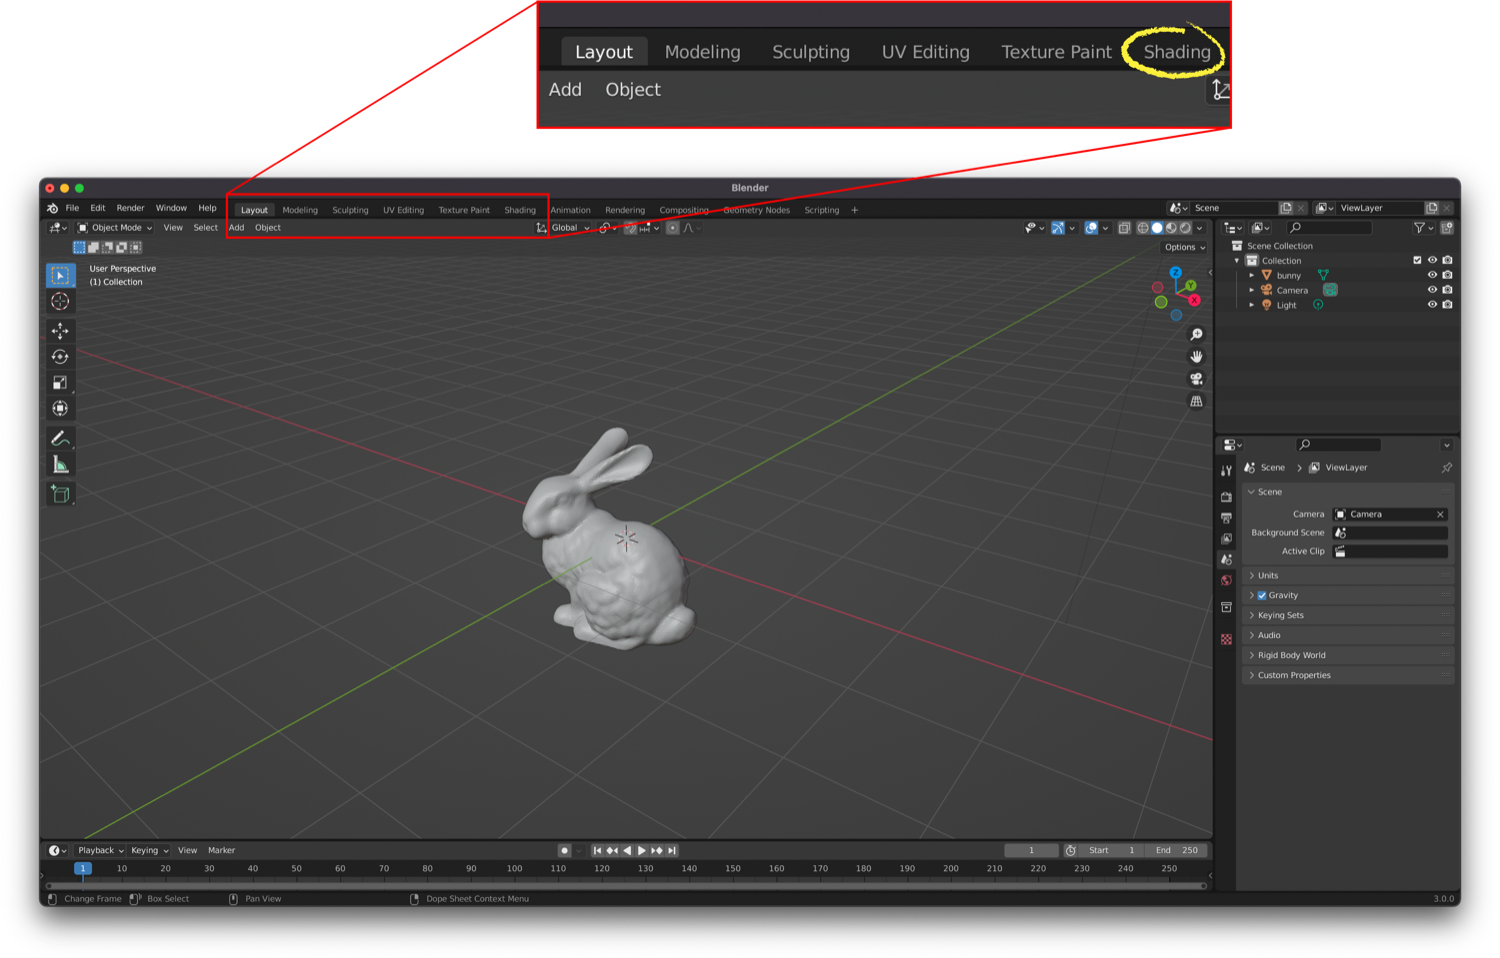
\includegraphics[width=0.9\textwidth]{images/shader_tab.png}
         \caption{The location of the \Menu[t>]{Shading} tab.}
         \label{subfig:shading_tab_a}
        \end{subfigure} \\
        \begin{subfigure}[b]{0.9\textwidth}
         \centering
         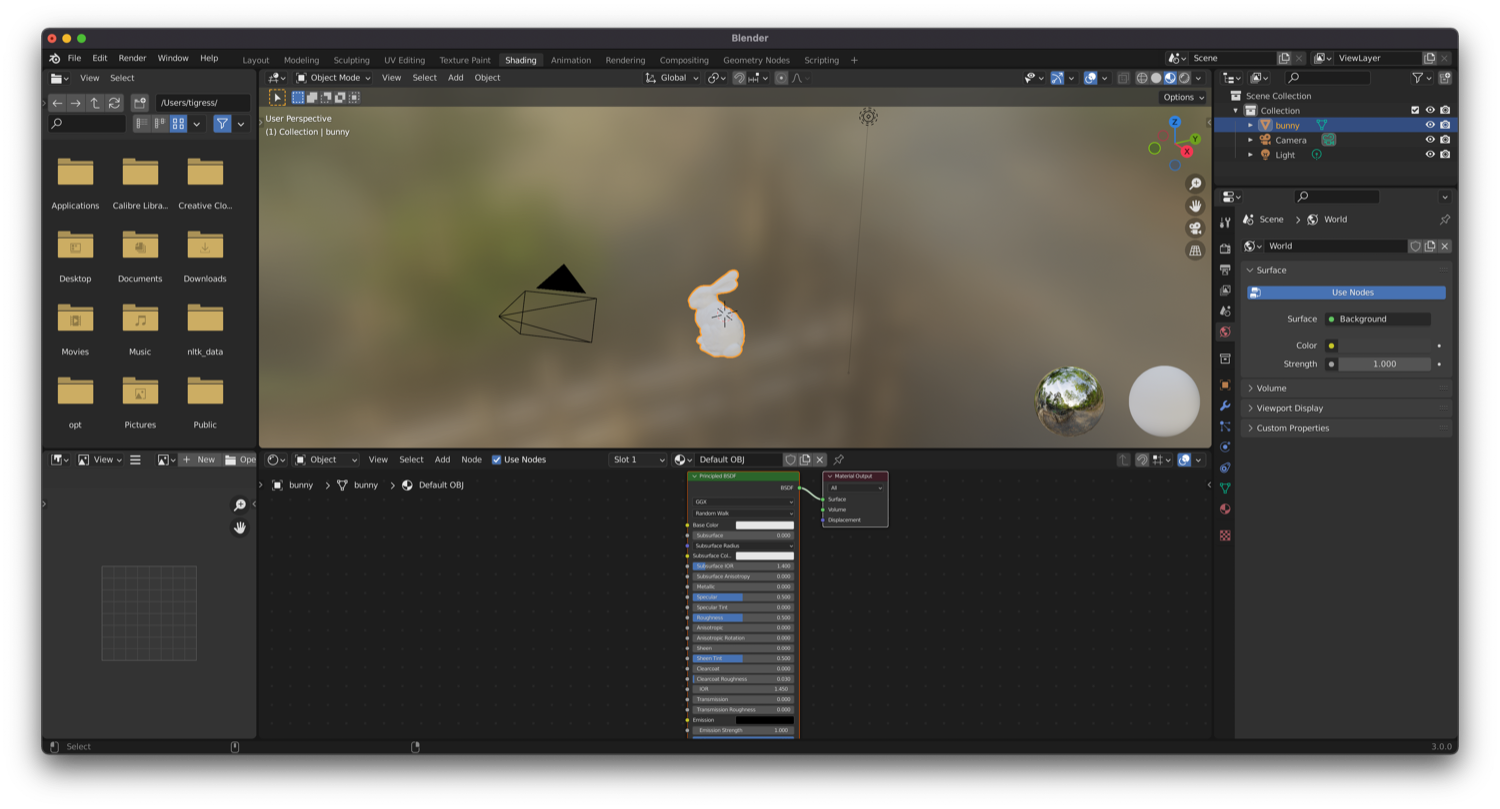
\includegraphics[width=0.9\textwidth]{images/2022-06-17_shading-editor.png}
         \caption{The Shading editor.}
         \label{subfig:shading_tab_b}
        \end{subfigure}
        \caption{Clicking the \Menu[t>]{Shading} tab (\ref{subfig:shading_tab_a}) brings up the Shading editor (\ref{subfig:shading_tab_b}.)}
        \label{fig:shading_tab}
    \end{figure}
    \item Once the target mesh is selected, you can add shading nodes. \keys{shift + A} is the keyboard shortcut to \directory{Add} a node. When you press \keys{shift + A}, a menu will appear containing the different options. You can either manually click through the menu to find the node you want, or type in the search bar (the latter is faster.) Add a \obj{UV Map} node, which gets the UV map associated with the mesh we imported.
    \item By default, Geometry Central stores scalar data in the first uv coordinate. Add a \obj{Separate XYZ} node, and hook the \obj{UV Map} node up to \obj{Separate XYZ}; then hook up the {\tt `X'} field of \obj{Separate XYZ} to the {\tt `Base color'} field of the \obj{Principled BSDF} node, which feeds just the first coordinate of the UV map as a color value to the mesh (see Figure~\ref{fig:uv_separateXYZ}.) Your editor should look something like Figure~\ref{fig:uv_separateXYZ}.
    \begin{figure}[H]
        \centering
        \captionsetup{width=0.8\textwidth}
        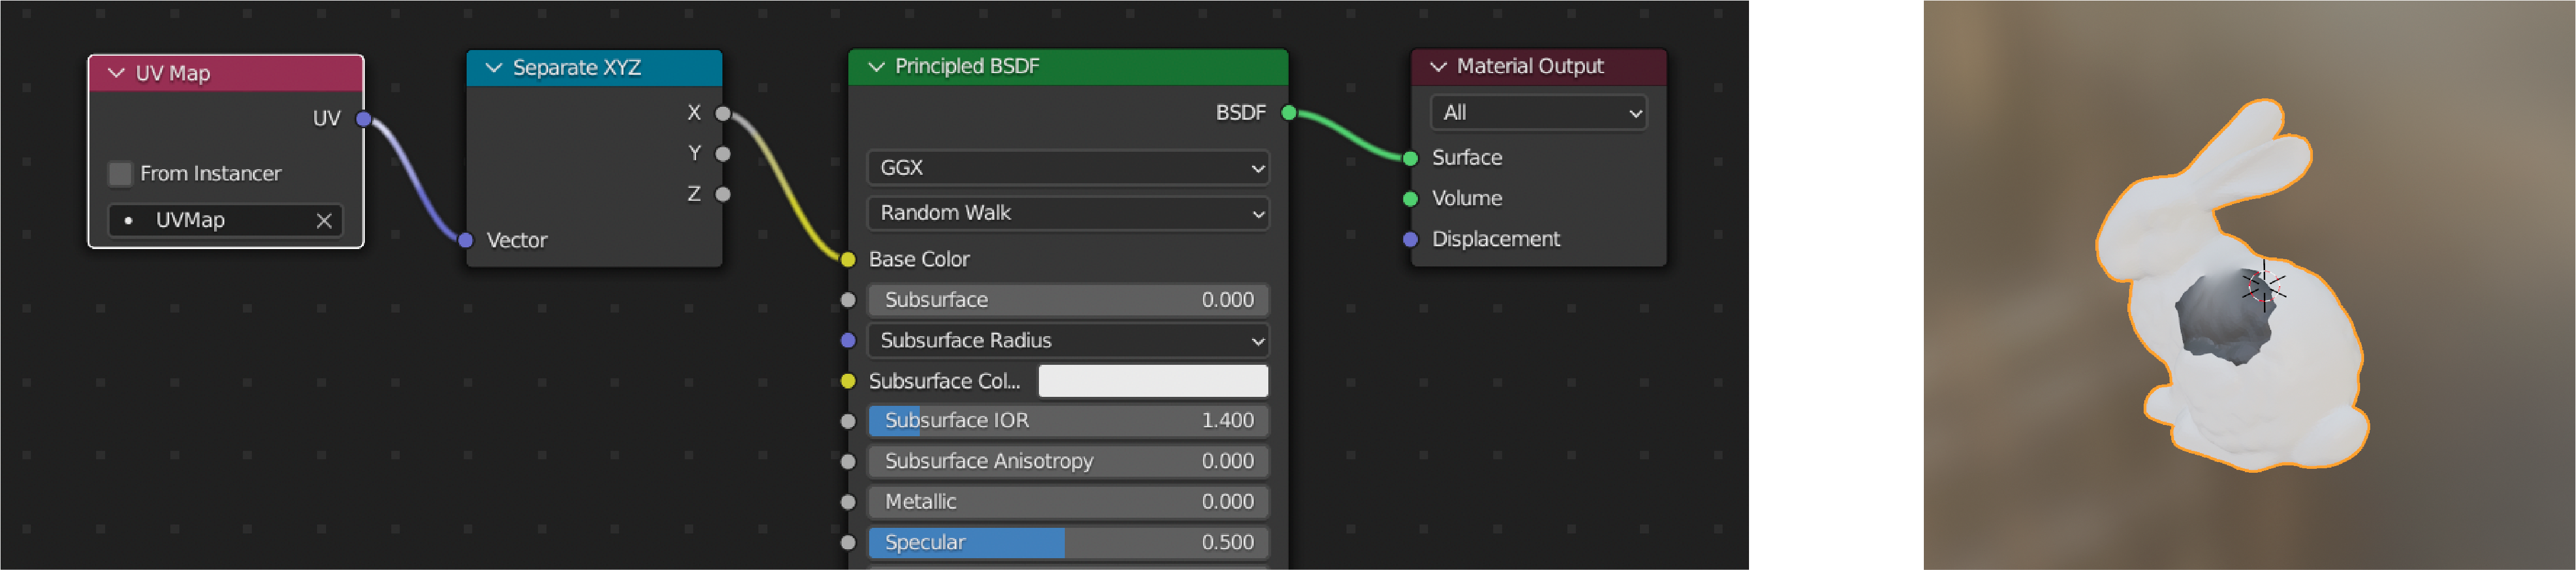
\includegraphics[width=0.8\textwidth]{images/scalar-data-shading-nodes.png}
        \caption{The sequence of nodes that gets our scalar data to show on our surface mesh. (The scalar data in this example is just a simple diffusion curve on the bunny.)}
        \label{fig:uv_separateXYZ}
    \end{figure}
    \item Add a \obj{ColorRamp} node after \obj{Separate XYZ} and feed its color output to the base color of the mesh, to map the scalar data onto a custom color range. 
    \begin{figure}[H]
        \centering
        \captionsetup{width=0.8\textwidth}
        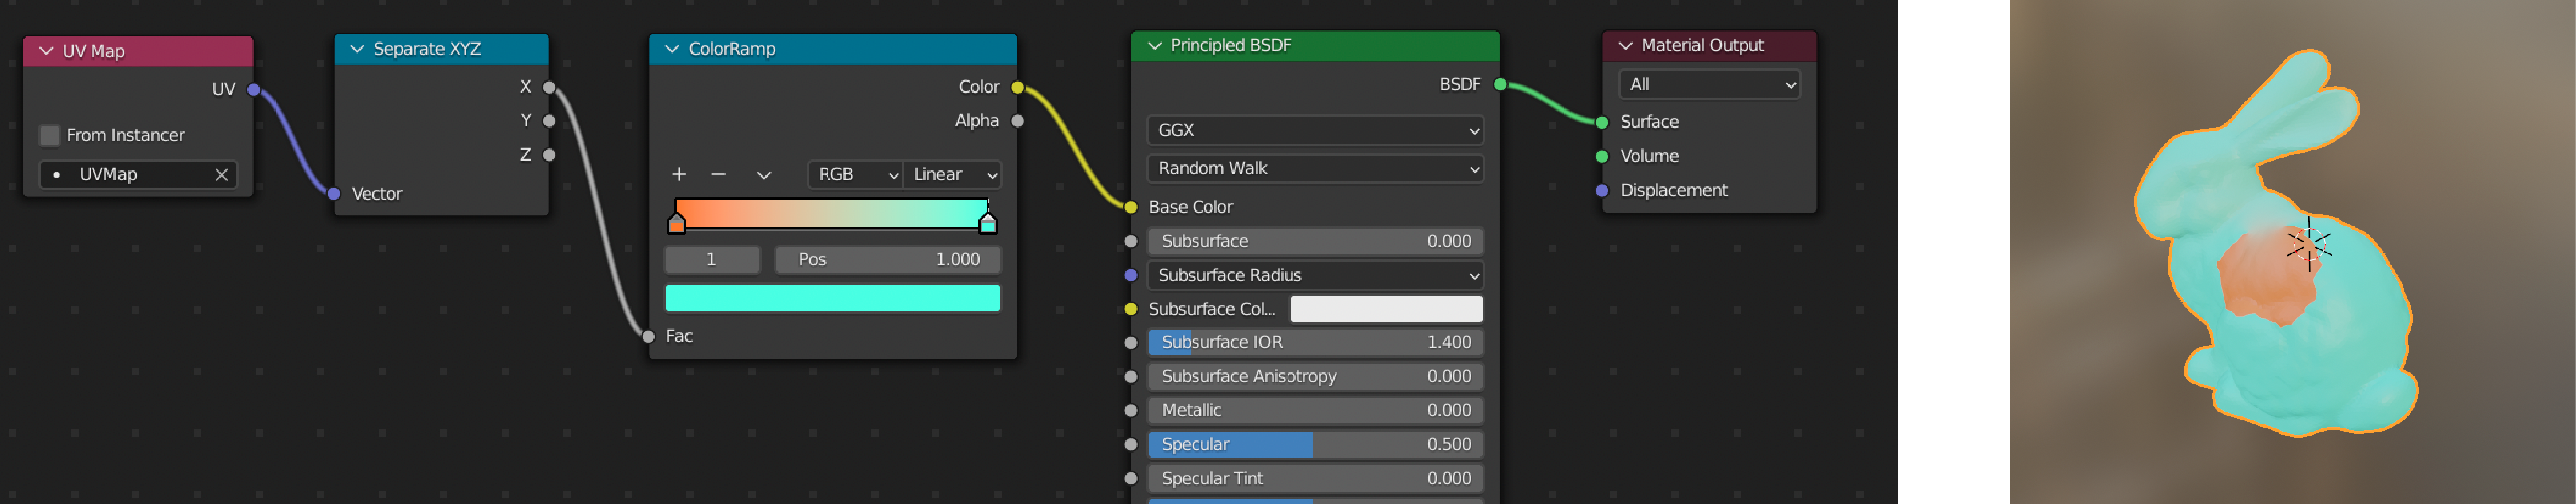
\includegraphics[width=0.8\textwidth]{images/scalar-data-colorramp.png}
        \caption{Customizing the colormap used to display the scalar data.}
        \label{fig:uv_separateXYZ_colorramp}
    \end{figure}
    \item Currently, the mesh looks polygonal (I mean, because it is, but most of the time we want smooth shading.) In \directory{Object} menu button in the upper left of the viewport, click \directory{Shade smooth} for smooth shading (Figure~\ref{fig:shade_smooth_bunny}.)
    \begin{figure}[H]
        \centering
        \captionsetup{width=0.8\textwidth}
        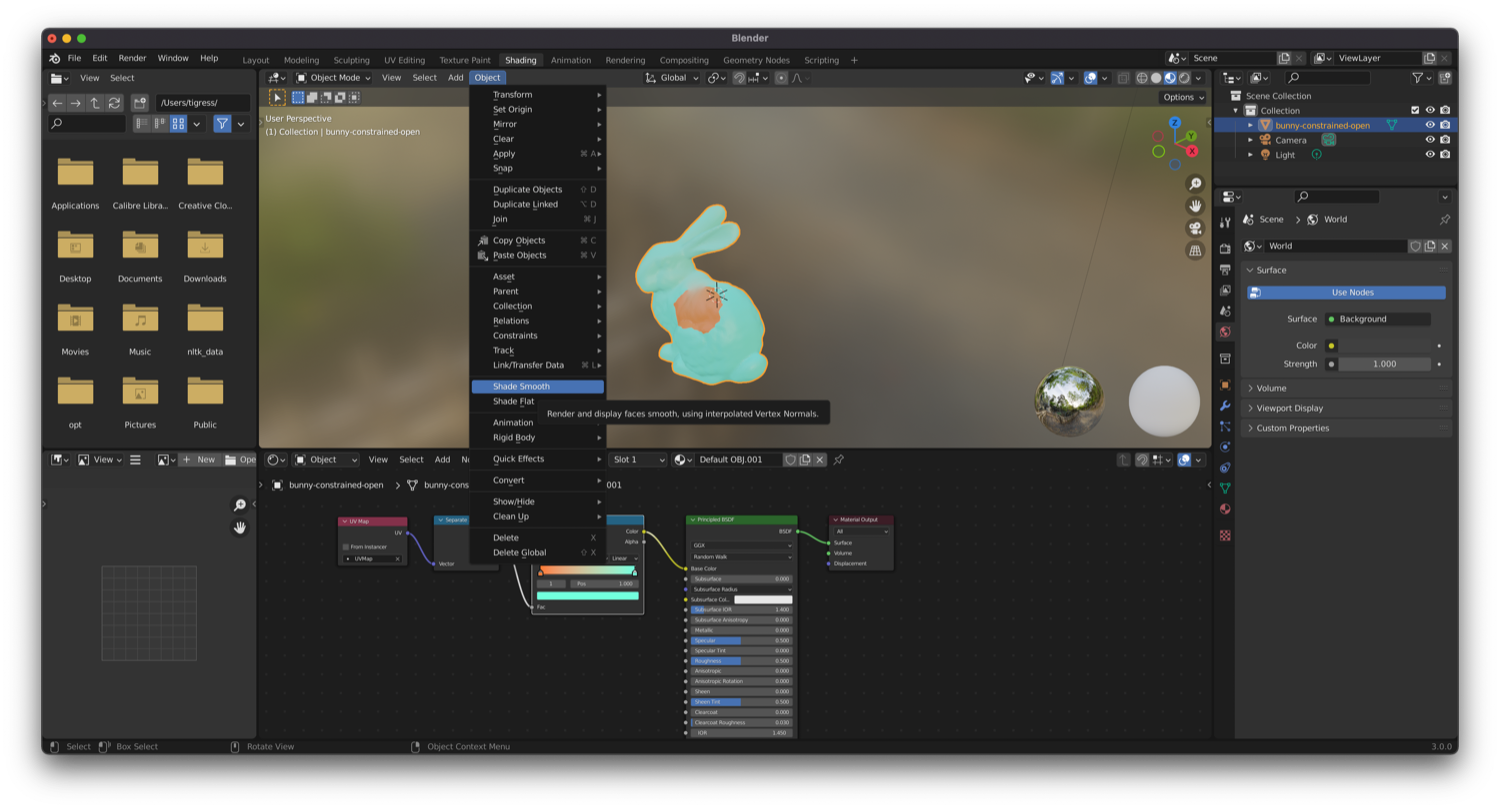
\includegraphics[width=0.8\textwidth]{images/2022-06-17_shade-smooth-bunny.png}
        \caption{Click \directory{Object / Shade smooth} for smooth shading.}
        \label{fig:shade_smooth_bunny}
    \end{figure}
    \item For better rendering quality, go to \menu{Properties > Render properties} (\inlinepic{images/2022-06-17_render-properties-icon.png} in the right panel menu.) For ``Render Engine'', select ``Cycles'' instead of ``Eevee''. An example render is shown in Figure~\ref{fig:scalar-data-final}:
    \begin{figure}[H]
        \centering
        \captionsetup{width=0.8\textwidth}
        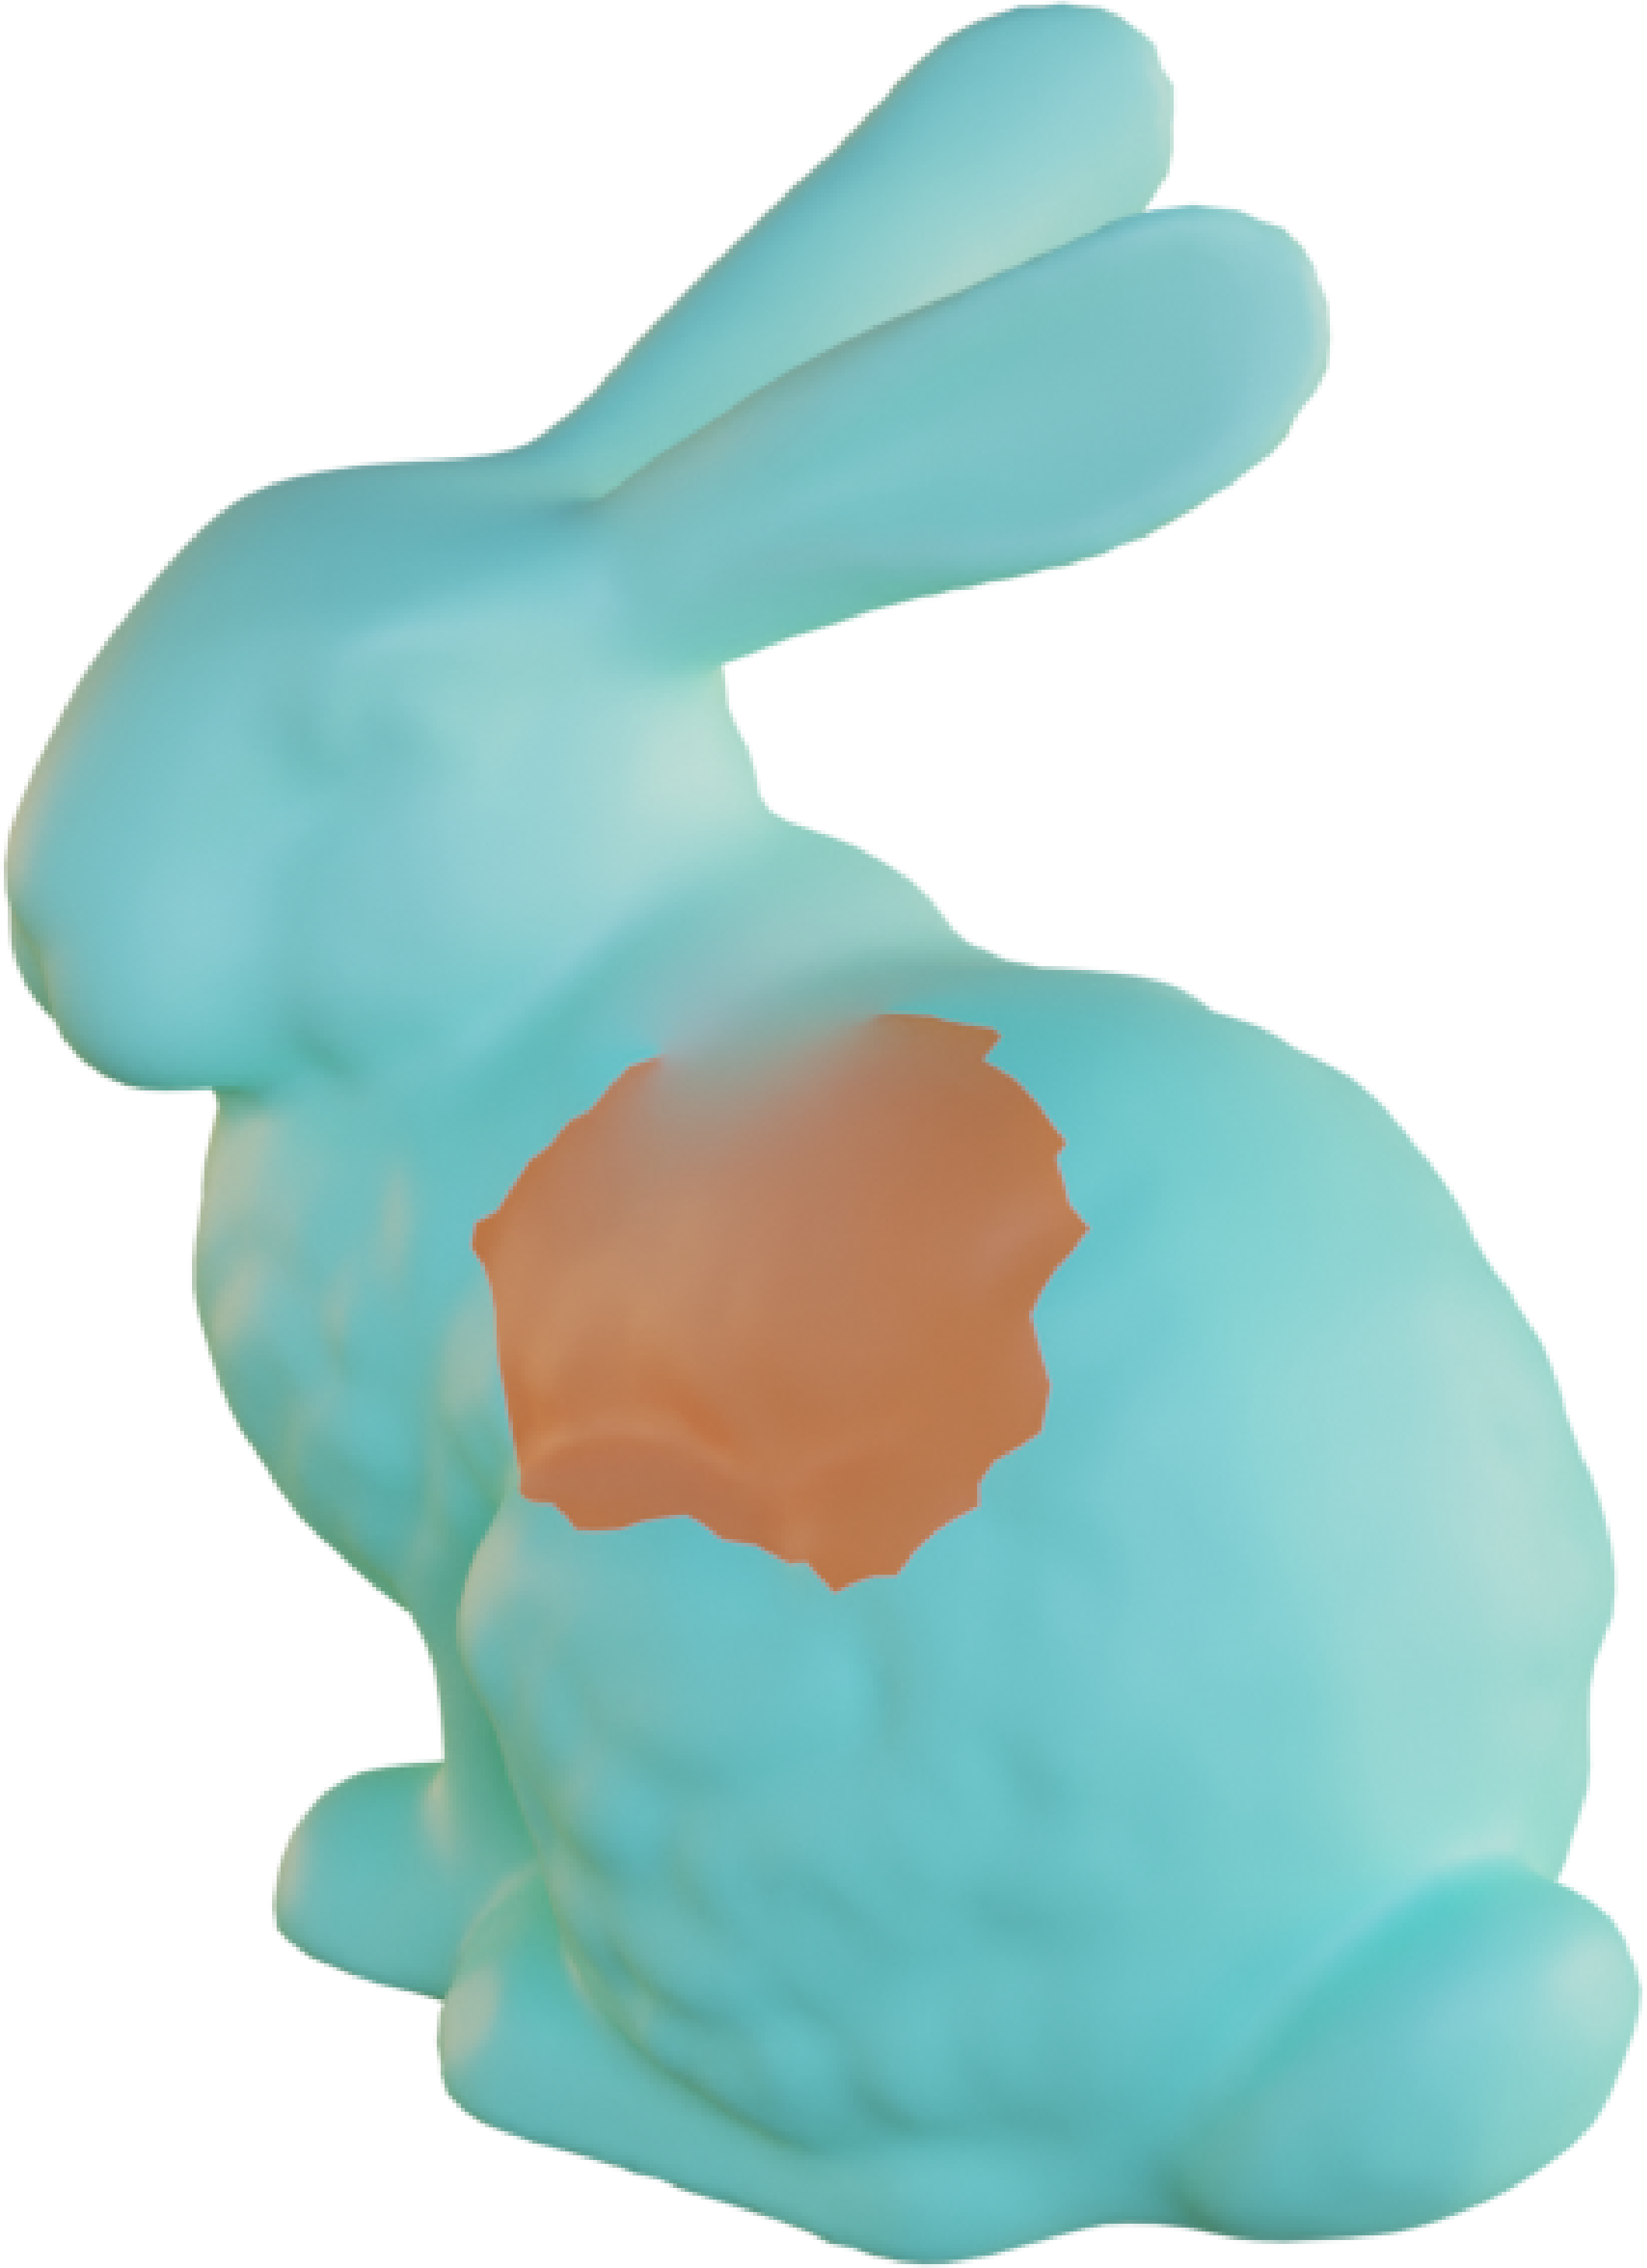
\includegraphics[width=0.3\textwidth]{images/scalar-data-final.png}
        \caption{A render, using the ``Courtyard'' environment texture for lighting. I prefer not to use environment lights when rendering figures for papers, but this is just preference. See Section~\ref{sec:Lighting} for lighting methods.}
        \label{fig:scalar-data-final}
    \end{figure}
    \item For material options, see Section~\ref{sec:Materials}.
    \item In this example, we only visualized a gradient between two values -- for tips on visualizing more complicated scalar functions, see Section~\ref{sec:FunctionVisualization}. Important for visualizing functions on surfaces: Lights and materials can interact in unexpected ways to affect the saturation and lightness of the colors in your texture. If you are planning to display colormapped data on your surface next to a colorbar legend, you should probably add additional items to your shader to ensure accurate colors; see Section~\ref{sec:FunctionVisualization}. 
\end{enumerate}

\section{Rendering points}
\textbf{TODO:} You can write an OBJ file with vertex positions, then render the points by instancing a sphere, cube, etc. at each vertex.

\section{Rendering vector data}
\textbf{TODO:} Vectors on vertices, edges, faces. Little vectors with arrows, or streamlines.

When your data gets more complicated, there is typically more information you want to specify than can be stored in an OBJ file. For example, for a vector field you want to specify (1) the 3D positions of each vector; (2) RGB colors for each vector; (3) possible more information for each vector...

A common approach to store the extra information is to co-opt the texture coordinates and normal information in an OBJ file. Personally, I find it's easier to simply store all this info as the vertex positions of a *separate* OBJ file -- this approach has the benefit that you don't have to re-write your OBJ file representing your mesh every time you simply make a change in how you want the mesh to be rendered. It also seems easier to me to explicitly keep track of each type of quantity you're using to render the mesh, though of course it's possible to update the instructions that follow to take different types of input.

\subsection{Vector fields}
\label{sec:VectorFields}
To render a vector field, typically you want to display a little arrow for sampled point in a domain. We will do this in Blender via \emph{instancing}, which copies an object to multiple points. Once arrows have been instanced to each sample point, we can display our vector field by controlling the local rotation of each arrow. One way to do that is to write out each arrow's direction in world coordinates (meaning as a vector in $\R^3$), read data from this file via a script in Blender, and use the \obj{Align Euler to Vector} node to align each arrow to the corresponding direction. In what follows below, I will describe the process of rendering tangent vectors on a surface mesh --- though this process can also be adapted to the (simpler) process of rendering a collection of vectors in a 3D volume.

I save the vectors encoding rotation information in an OBJ file, with the vectors as vertex positions --- I personally find this the most straightforward way to get collections of 3-tuples into Blender. A straightforward way to display a vector field is to have one vector per vertex or face, although for finely-tessellated meshes this will produce a vector field that is too densely sampled and makes for a poor visualization. A better approach is to use some method for \href{https://www.cs.ubc.ca/~rbridson/docs/bridson-siggraph07-poissondisk.pdf}{Poisson Disk Sampling}, which was used, for instance, in the \href{https://www.cs.cmu.edu/~kmcrane/Projects/VectorHeatMethod/paper.pdf}{Vector Heat Method paper} --- I've implemented Poisson disk sampling in the C++ geometry processing library \href{https://geometry-central.net/surface/algorithms/surface_sampling/}{geometry-central}, though similar variants are implemented other software (\href{https://www.meshlab.net/}{MeshLab}, for one.)

\begin{enumerate}
    \item For better control of geometry in Blender, we can use Geometry Nodes. The Geometry Nodes editor can be accessed by clicking the \Menu[t>]{Geometry Nodes} tab (shown in Figure~\ref{fig:geometry-nodes_tab}.)
    \begin{figure}[H]
        \centering
        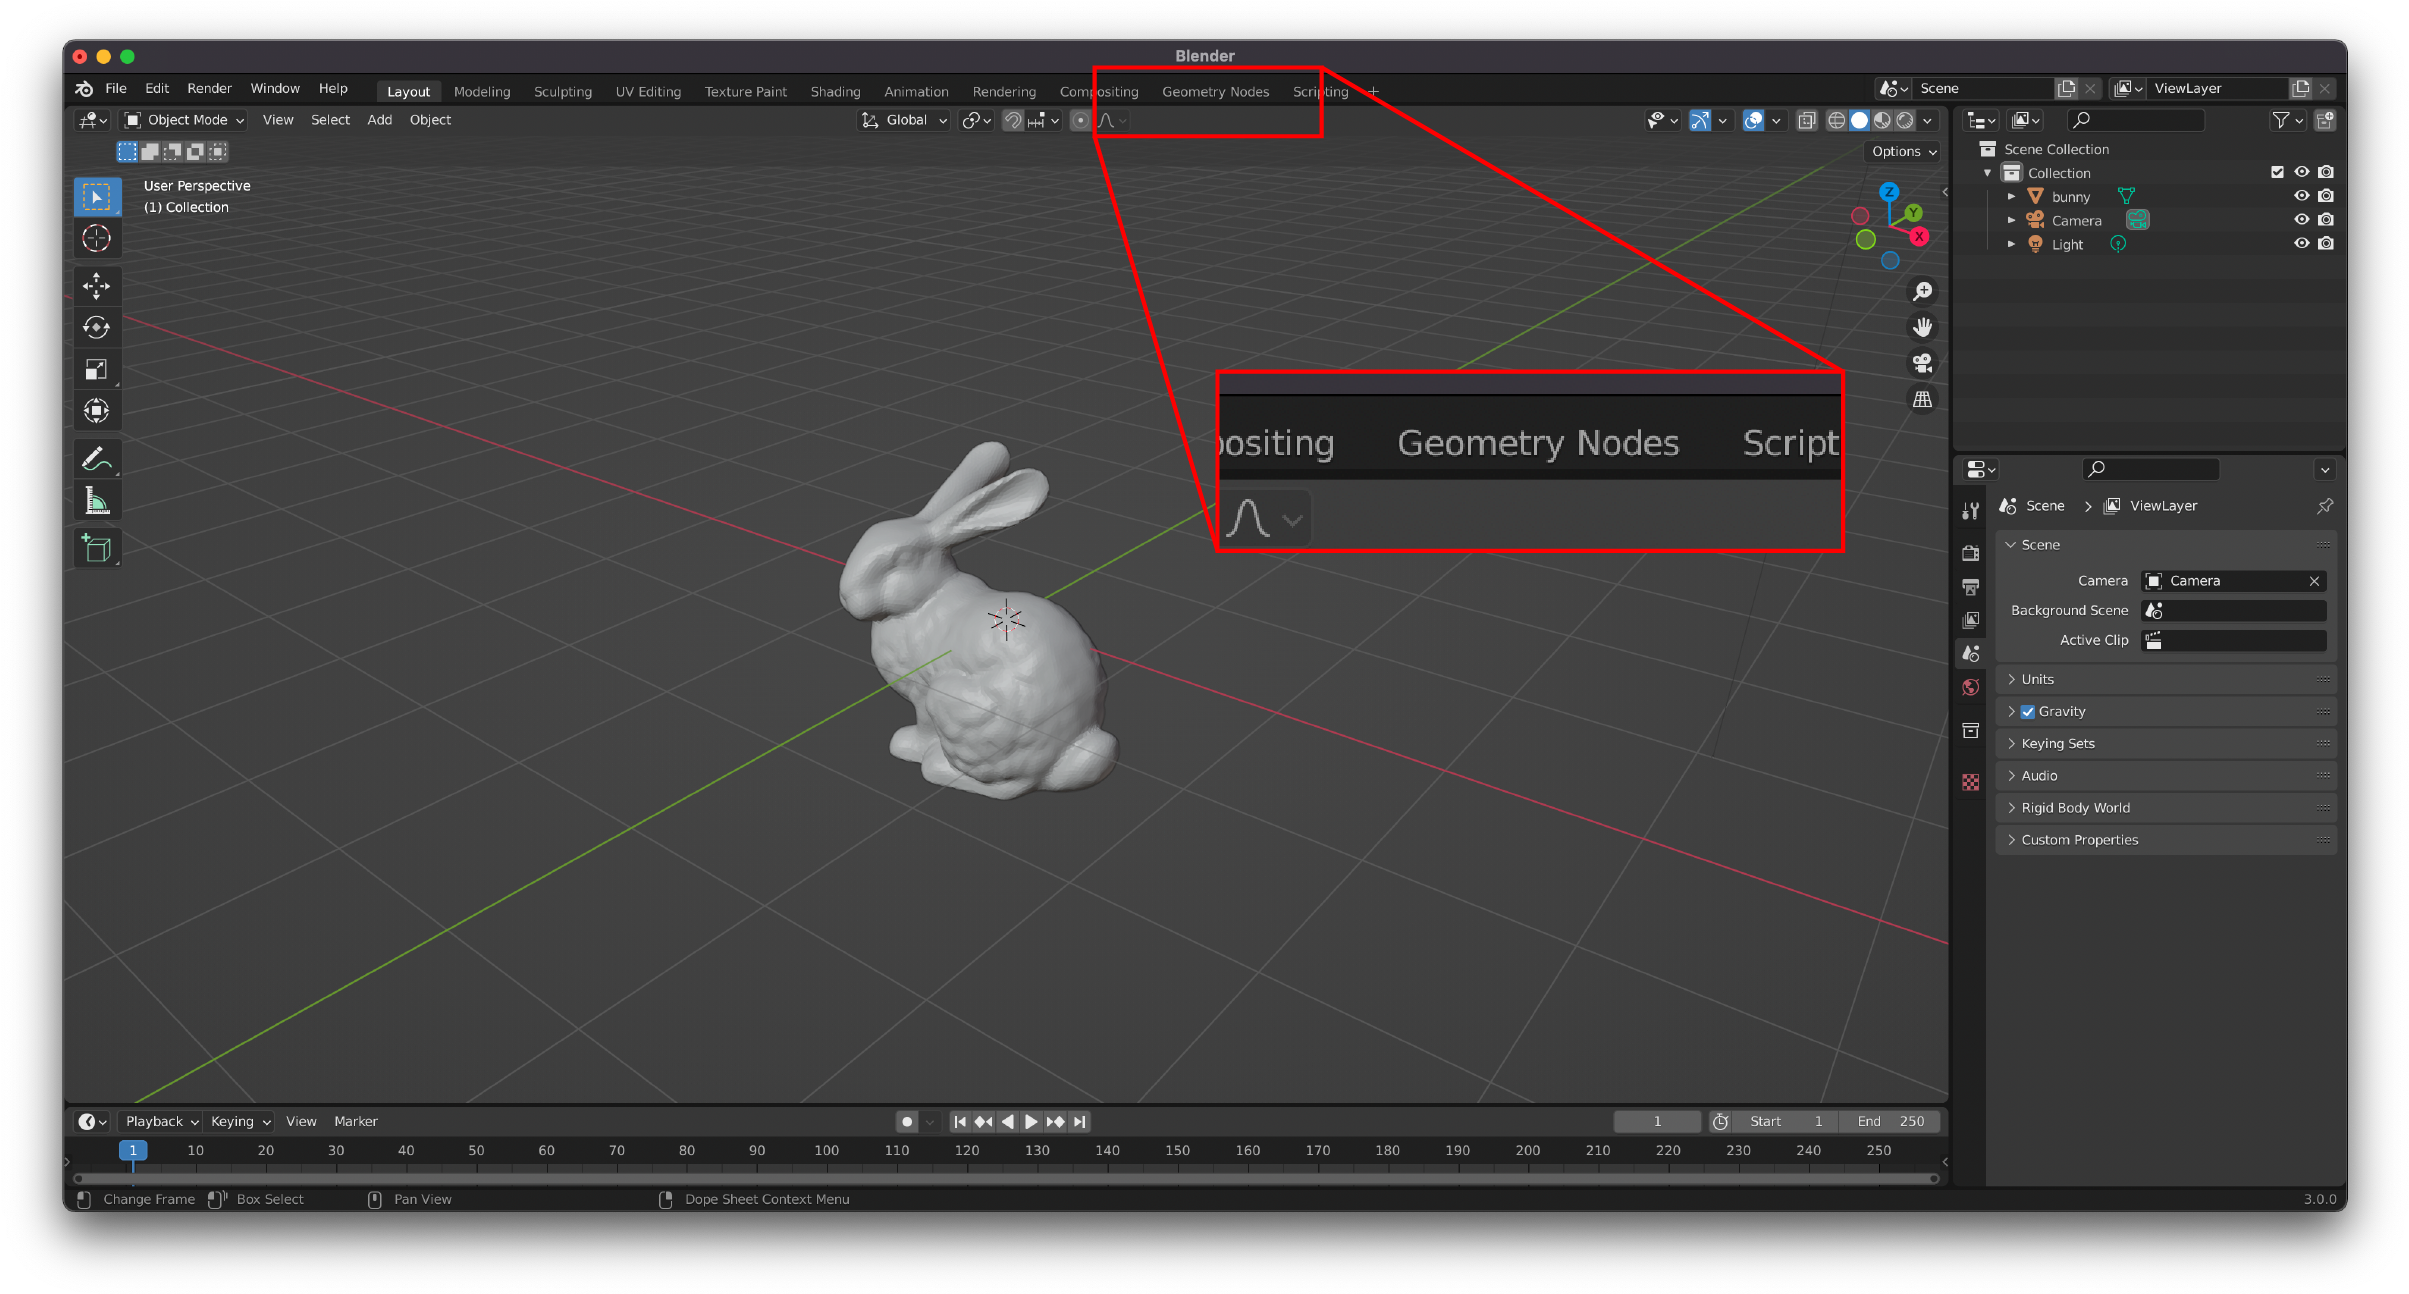
\includegraphics[width=0.9\textwidth]{images/geometry-nodes-tab.png}
        \caption{The location of the \Menu[t>]{Geometry Nodes} tab.}
        \label{fig:geometry-nodes_tab}
    \end{figure}
    \item Import two items: the mesh, and the arrow object you want instanced. You probably want to choose a simplified arrow representation to make the visualization more clear, such as the compass-needle-like arrow used in the \href{https://www.cs.cmu.edu/~kmcrane/Projects/VectorHeatMethod/paper.pdf}{Vector Heat Method paper.}
    
    In this example, I've imported a kitten mesh and a teardrop-needle shape similar to the one used in the Vector Heat Method (Figure~\ref{fig:vector_instance_meshes}.)
    \begin{figure}[H]
        \centering
        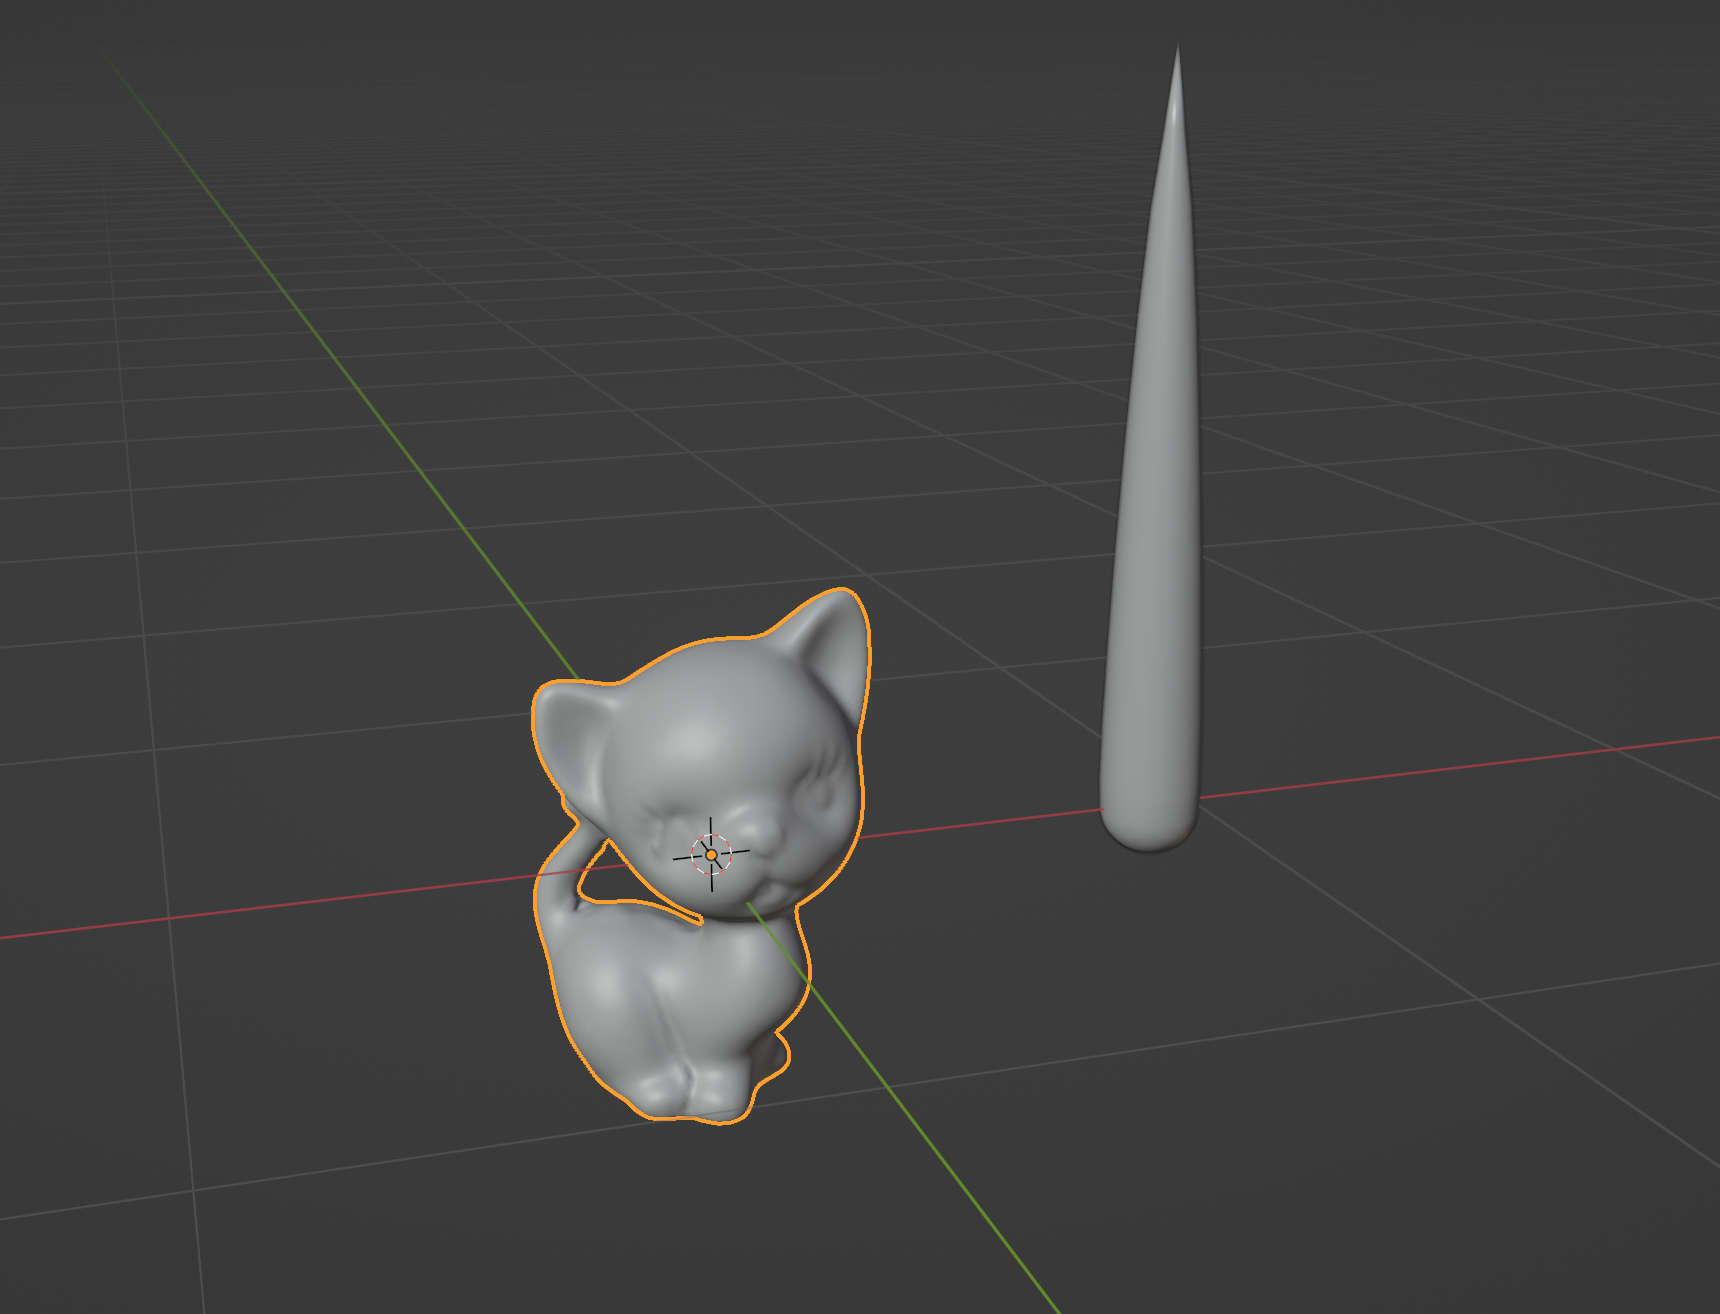
\includegraphics[width=0.5\textwidth]{images/vector_instance_meshes.png}
        \caption{The surface mesh used in this example (kitten) and the mesh used to represent the arrows.}
        \label{fig:vector_instance_meshes}
    \end{figure}
    You can toggle the visibility of each object in the \Menu[t>]{View Layers} menu in the upper right (see Figure~\ref{fig:view_layers_menu}.) Toggline the eye icon controls the visibility of the item in the viewport, and the camera icon controls the item's visibility in the render. We want to set the arrow object to non-visible in the final render, and also in the viewport to avoid being distracted by it.
    \begin{figure}[H]
        \centering
        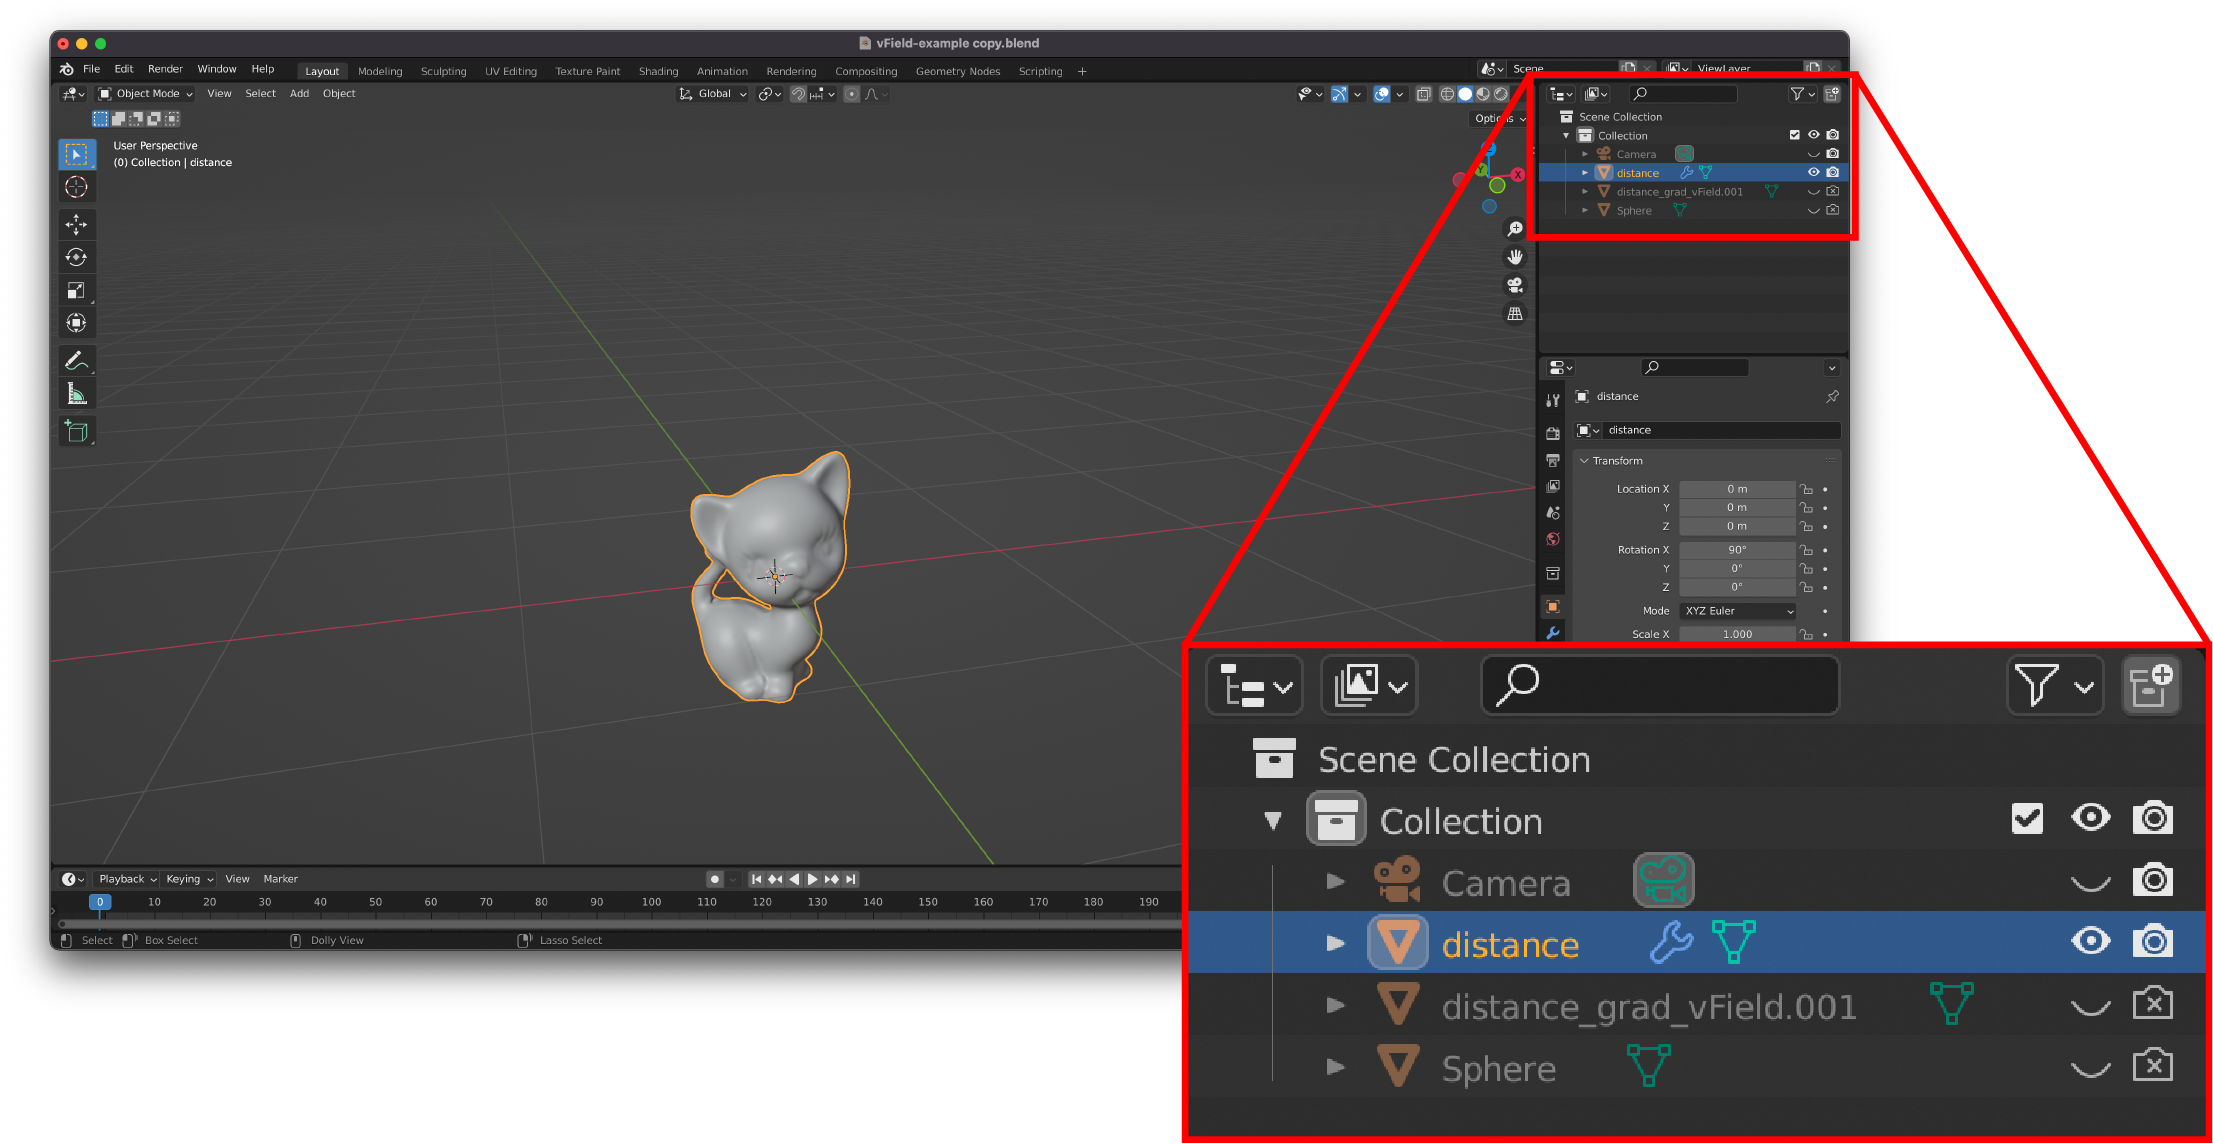
\includegraphics[width=0.8\textwidth]{images/view_layers_menu.png}
        \caption{The default position of the \Menu[t>]{View Layers} menu.}
        \label{fig:view_layers_menu}
    \end{figure}
    \item Select the mesh representing your surface. In the Geometry Nodes editor, click ``New''. You will see two initial nodes: \obj{Group Input} and \obj{Group Output}. The ``Geometry'' slot of \obj{Group Input} contains the currently-selected geometry, and any geometry that you want rendered must be eventually fed into \obj{Group Output}.
    \item Add two nodes: \obj{Mesh to Points} and \obj{Instance on Points}. (Beware: There is a very similarly-named node called ``Instance to Points''. You want ``Instance {\bf on} Points.'') In the \obj{Mesh to Points}, select the mesh element you want to instance to (e.g. faces.) Feed its ``Points'' output into the ``Instances'' output of \obj{Instance on Points}, which will instance a yet-to-specified object to each Point. Finally connect both the instancing output and \obj{Group Input} to a \obj{Join Geometry} node to ensure that both the mesh and the instances get rendered. See Figure~\ref{fig:vector_instance_0}.
    \begin{figure}[H]
        \centering
        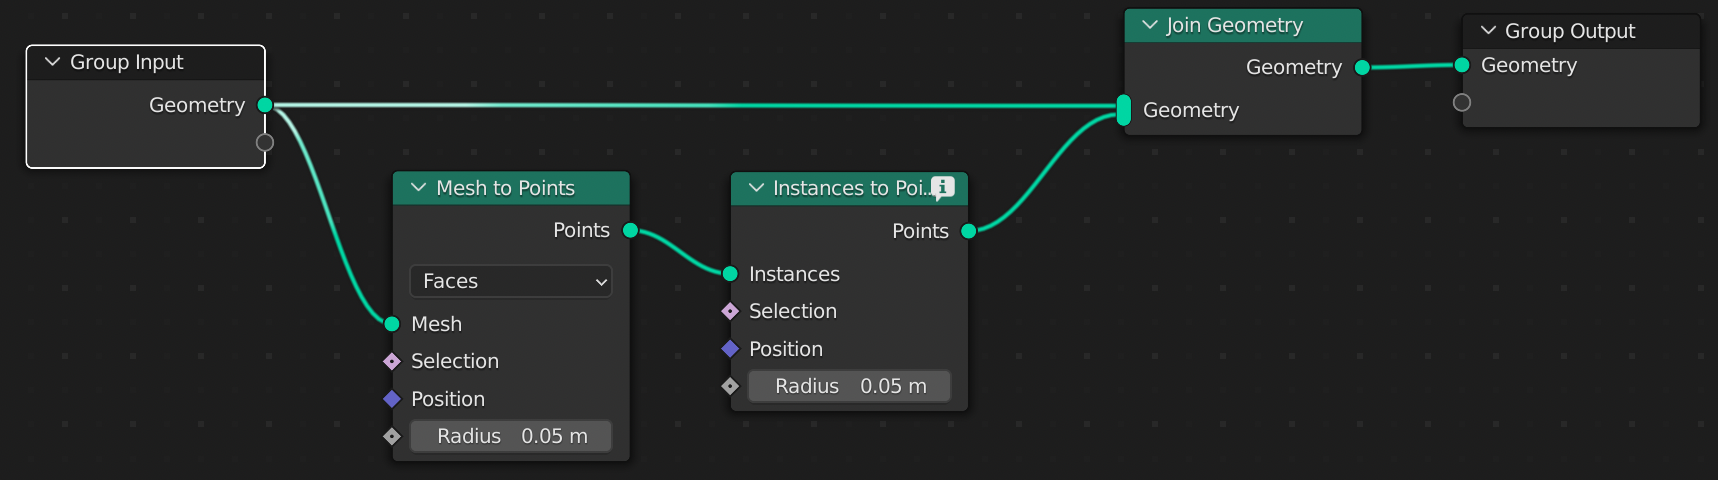
\includegraphics[width=0.8\textwidth]{images/vector_instance_0.png}
        \caption{Preparing to instance geometry.}
        \label{fig:vector_instance_0}
    \end{figure}
    \item Assuming the object you want instanced is already in the viewport, add an \obj{Object Info} node and select your object within this node. You can also add any other nodes modifying this object if you want; in this example, I've added a \obj{Shade smooth} node so I don't have to do it via the GUI. Your geometry nodes and viewport should now look something like this:
    \begin{figure}[H]
        \centering
        \captionsetup{width=0.8\textwidth}
        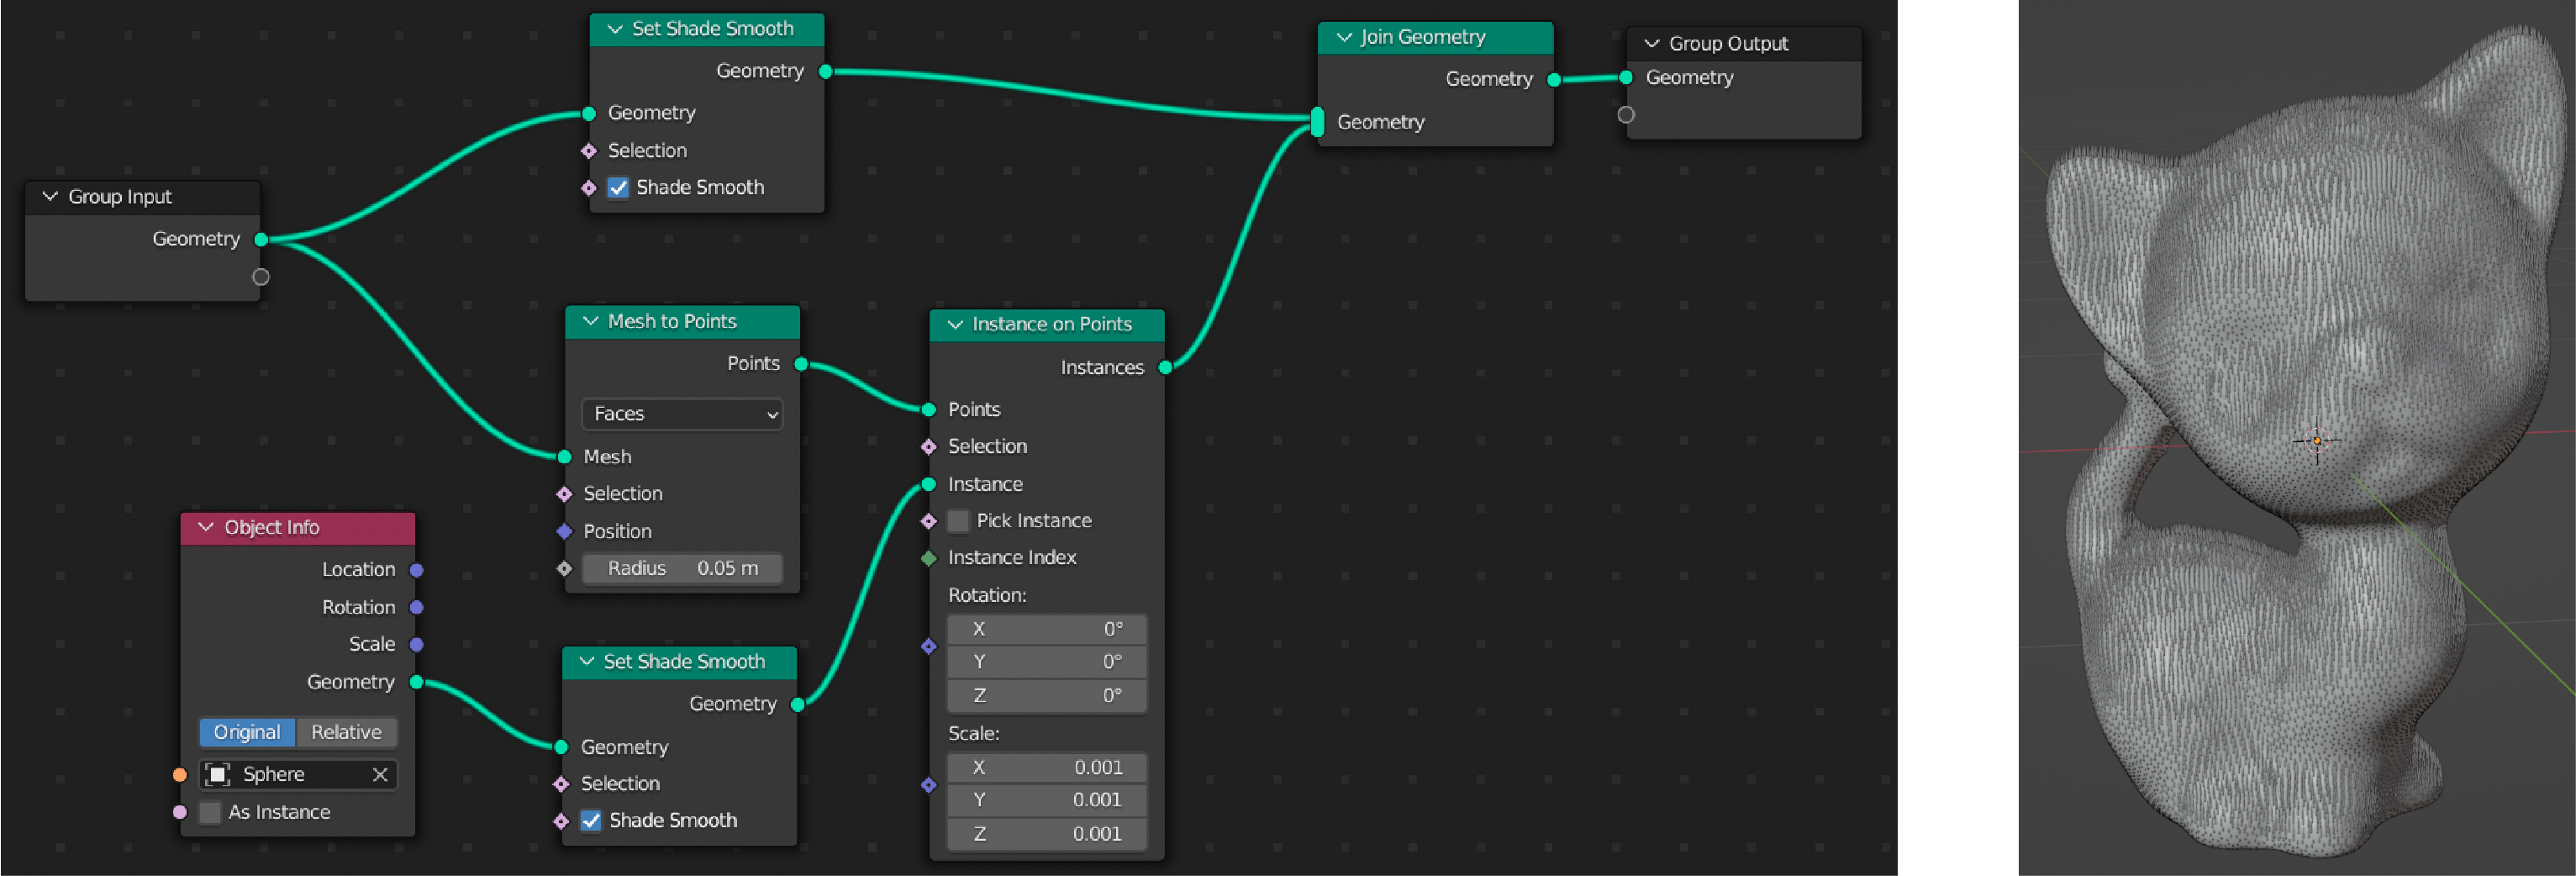
\includegraphics[width=0.9\textwidth]{images/vector_instance_1.png}
        \caption{Instancing the geometry. The arrow object is now instanced to every face in the kitten mesh. Their orientations haven't been set yet, so they're aligned to an arbitrary direction right now.}
        \label{fig:vector_instance_1}
    \end{figure}
    Since the arrow-needle object was so large to begin with, I scaled all instances down via the ``Scale'' fields in \obj{Instance on Points}.
    \item We could use a Python script to load in the rotation data -- and more generally, use a Python script to do all the Geometry Node manipulation -- but for a single example, it's fine to avoid scripting. 
    
    In this example, I've saved the rotation data for each face vector in a separate OBJ file, where the vectors are encoded as vertex positions. This is just an OBJ file with only vertex positions; there's no need to define a face, line, etc., and in fact adding extra connectivity info will slow Blender down a huge amount. 
    
    See Figure~\ref{fig:vector_instance_2} for the node configuration.
    \begin{figure}[H]
        \centering
        \captionsetup{width=0.8\textwidth}
        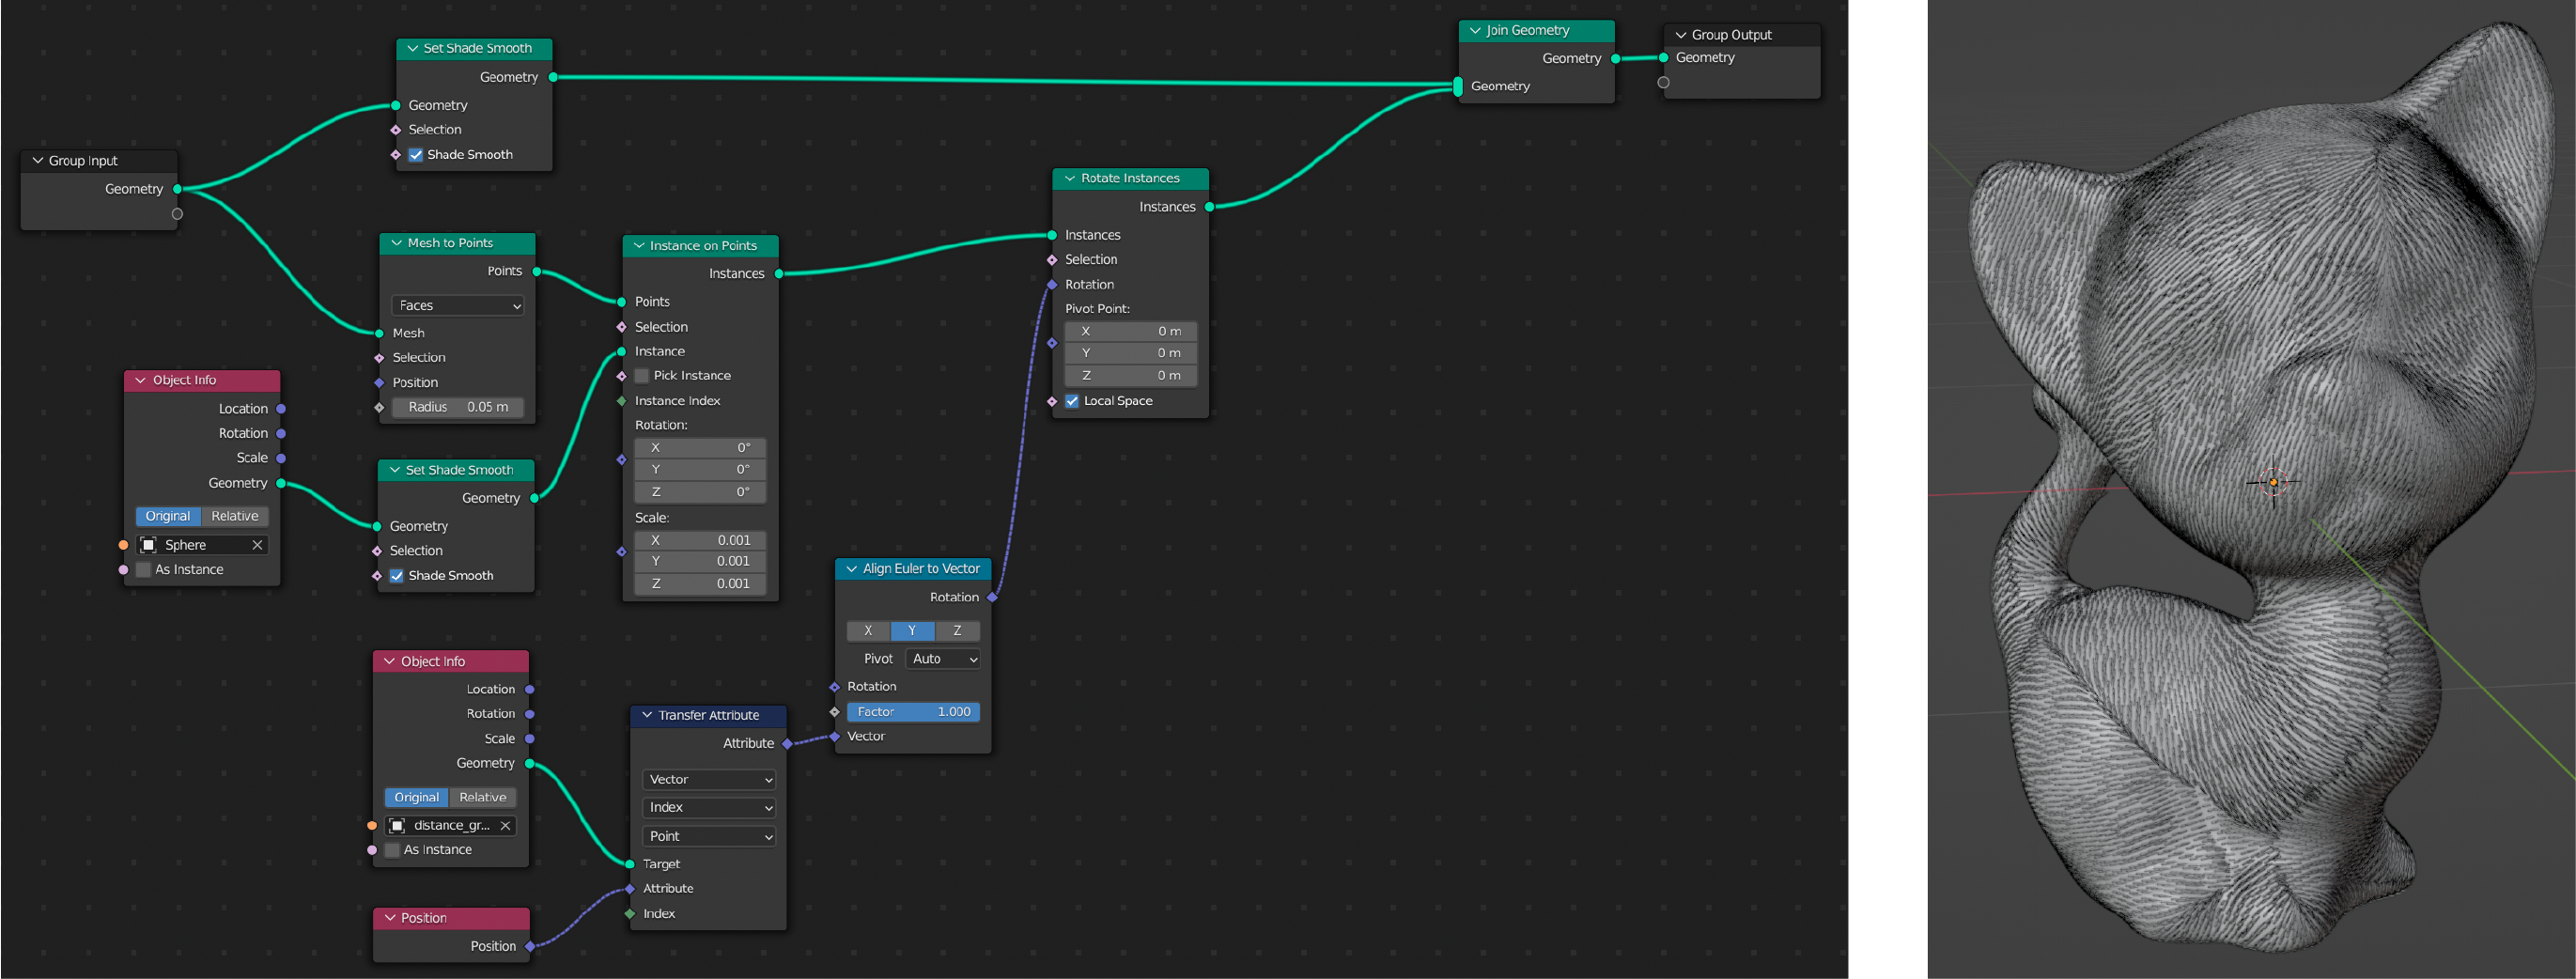
\includegraphics[width=0.9\textwidth]{images/vector_instance_2.png}
        \caption{Assigning directions to each vector. Now it's starting to look like our vector field!}
        \label{fig:vector_instance_2}
    \end{figure}
    
    Import the OBJ file containing the rotation info. Add the following nodes: \obj{Object Info}, \obj{Position}, \obj{Transfer Attribute}. In \obj{Object Info}, select the object corresponding to the rotation info. Feed this node and \obj{Position} into \obj{Transfer Attribute}, and set the data type to ``Vector'', mapping type to ``Index'', and domain to ``Point''. This transfers the position of vertices from the rotation object's geometry, which should have the same number of points as there are instances of the arrow geometry. (Note: In future versions of Blender (3.4+), the function of the \obj{Transfer Attribute} node has been incorporated into the \obj{Sample Index} node instead.)
    
    Add the nodes \obj{Align Euler to Vector} and \obj{Rotate Instances}. These two nodes in combination takes in the tangent vectors encoded by our fake rotation object, and produces a rotation that is aligned to the given direction, and aligns each instance to this direction. The ``Axis'' to align (X, Y, or Z) depends on the local axes of the original arrow object; in this example, it happens to be Y. 
    \item We also want to scale the arrows depending on their magnitude. Add a \obj{Vector Math} node, and set it to ``Length''. Feed in the attribute from \obj{Transfer Attribute} into \obj{Length}, and feed this length value into a \obj{Scale Instances} node as one of the components in ``Scale'' (Figure~\ref{fig:vector_instance_3}.)
    \begin{figure}[H]
        \centering
        \captionsetup{width=0.8\textwidth}
        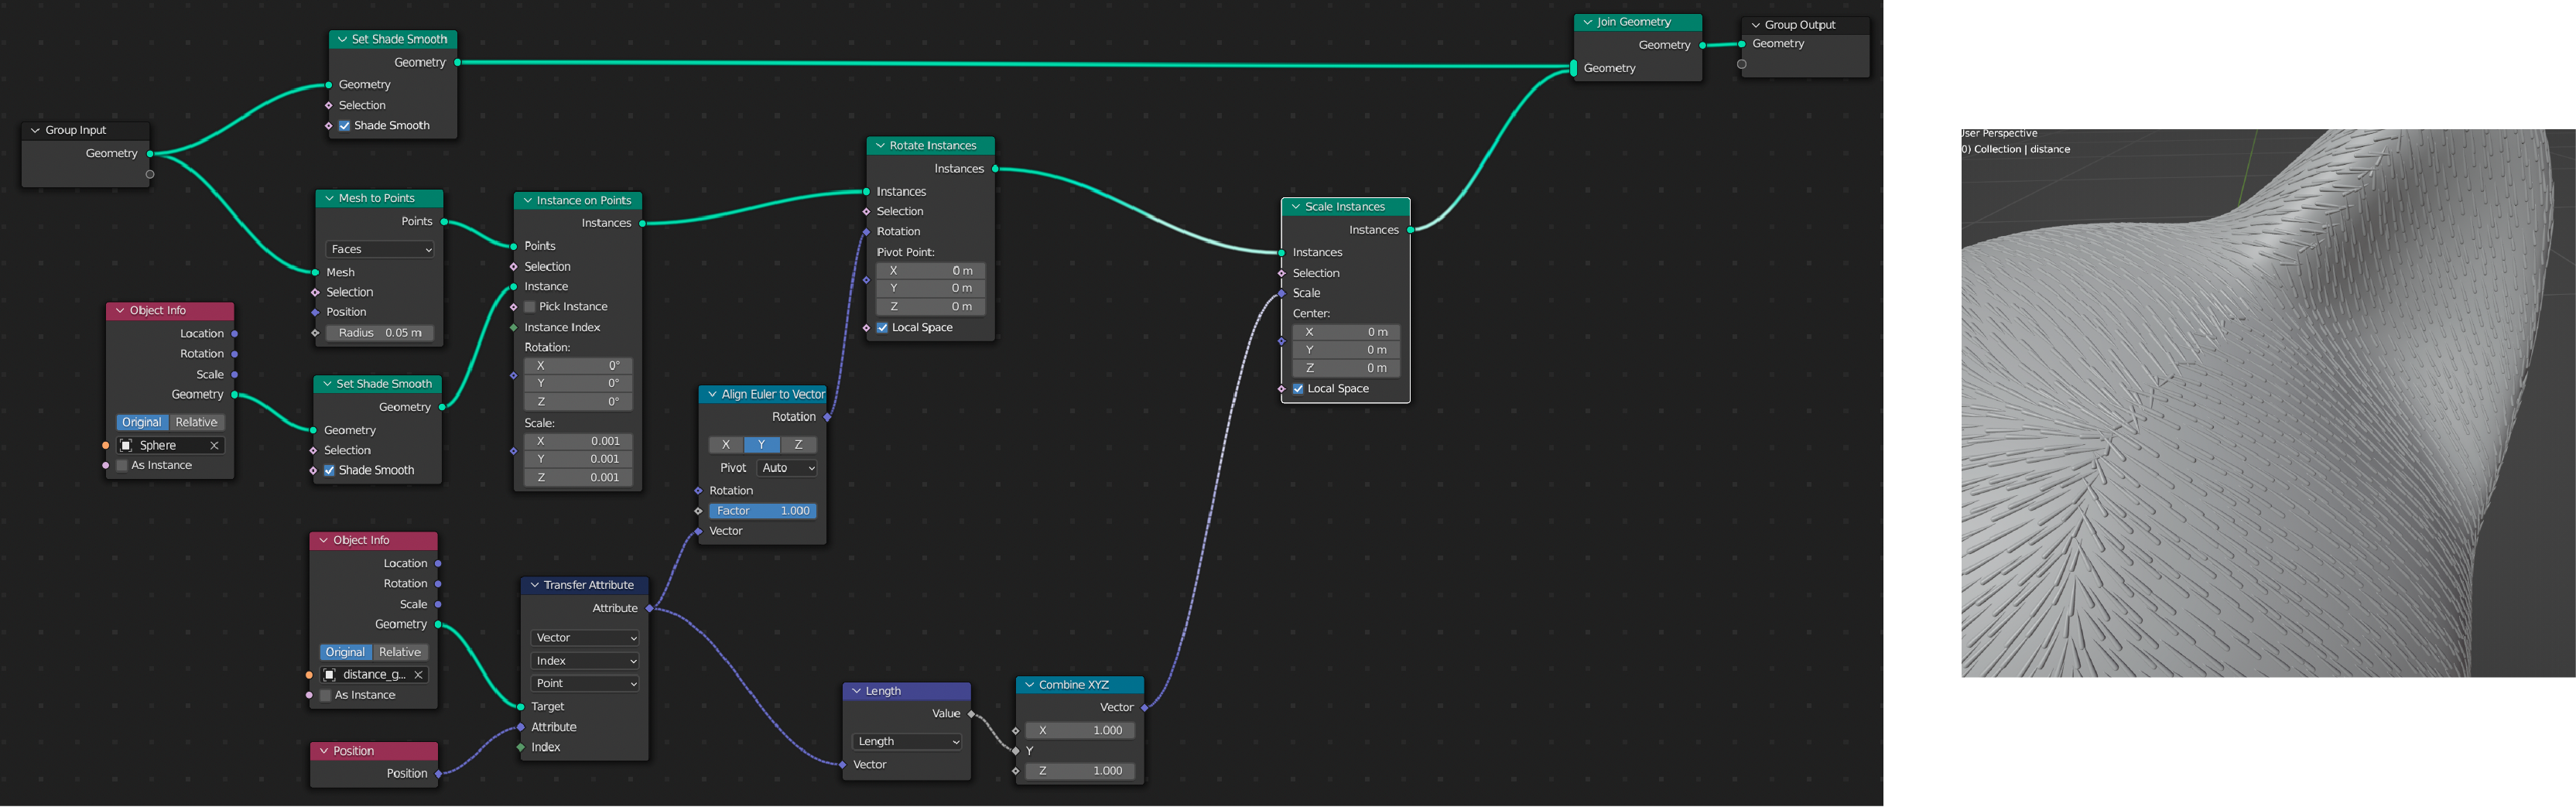
\includegraphics[width=0.9\textwidth]{images/vector_instance_3.png}
        \caption{Scaling the instanced arrows according to magnitude. In this example, not much changes because the vector field represents the gradient of an approximate distance field, so the magnitude is more or less unit everywhere; you would really have to zoom in to notice any changes. On the other hand, depending on the range of magnitudes in your vector field, you may need to impose another uniform scaling to make sure the arrows end up visible.}
        \label{fig:vector_instance_3}
    \end{figure}
    \item In this example, the arrow object was radially symmetric. However, if our arrow object was flattened, then simply aligning its longitudinal direction to the direction we input doesn't guarantee that the arrow also ``lies flat'' on the surface the way we want:
    \begin{figure}[H]
        \centering
        \captionsetup{width=0.8\textwidth}
        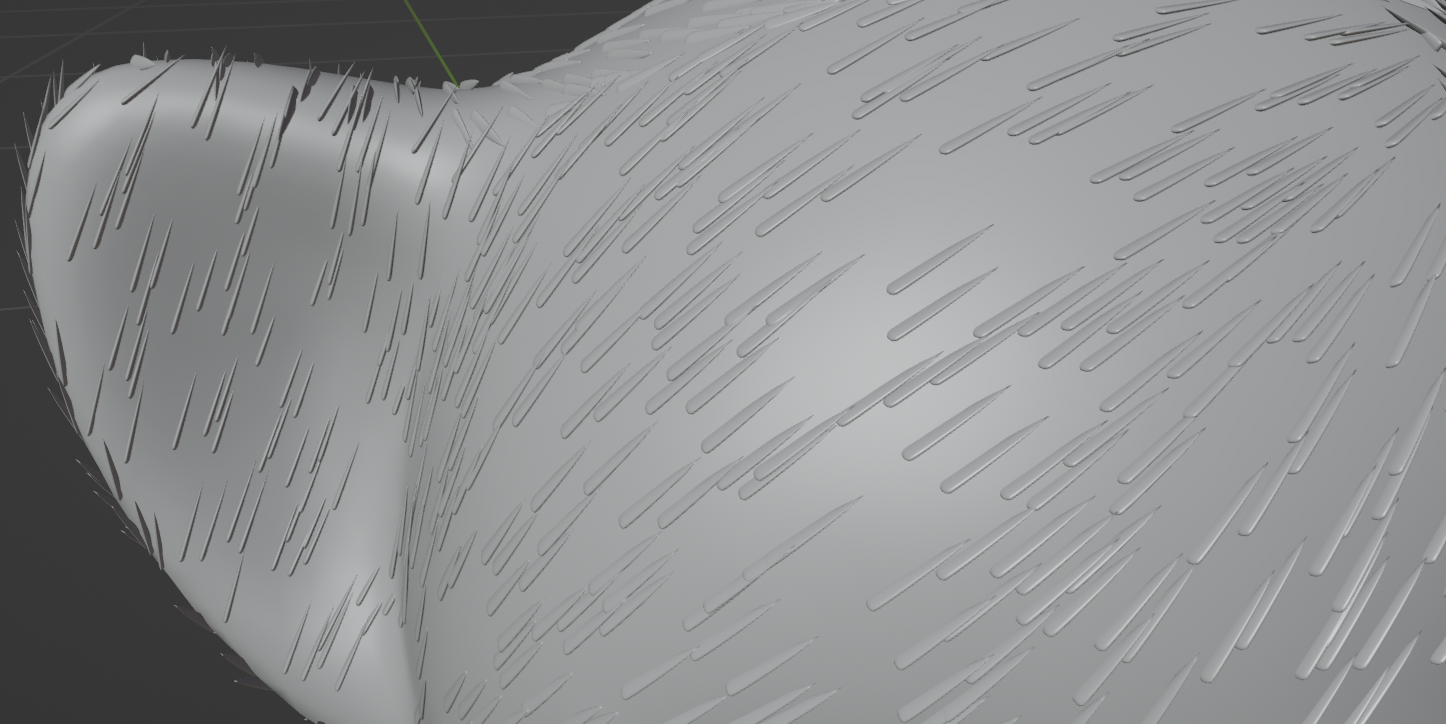
\includegraphics[width=0.7\textwidth]{images/vector_instance_non-adhering.png}
        \caption{For a non-symmetric object, the rotation that aligns one dimension to a given direction is non-unique. In particular, specifying that the longitudinal axis of a flattened arrow object should align with the given direction doesn't guarantee that the arrow lies flat along the surface -- this is particularly apparent on the ear of the kitten.}
        \label{fig:vector_instance_non-adhering}
    \end{figure}
    The solution is to add another \obj{Align Euler to Vector} node; this time, we want to align one of the transverse axes of the arrow to align with the normal of the surface. To get the normal of the surface, we use a \obj{Transfer Attribute} node like before, feeding in the surface geometry as input and a \obj{Normal} node. Again, make sure to select ``Vector'' as the data type in \obj{Transfer Attribute}. In this case, selecting ``Nearest Face Interpolated'' produces the same result as selecting ``Index'' and ``Face'' as the mapping and domain types, respectively. Finally, select the appropriate local axis of the arrow object to align in \obj{Align Euler to Vector}, and feed in its output rotation into the input rotation of the original \obj{Align Euler to Vector} node we used to rotate our arrows. 
    \begin{figure}[H]
        \centering
        \captionsetup{width=0.8\textwidth}
        \includegraphics[width=0.9\textwidth]{images/vector_instance_adhering_nodes.png}
        \caption{Adding nodes to additionally align our arrows to lie flat along the surface. New nodes and connections added in this step are indicated in red.}
        \label{fig:vector_instance_adhering_nodes}
    \end{figure}
    \begin{figure}[H]
        \centering
        \captionsetup{width=0.8\textwidth}
        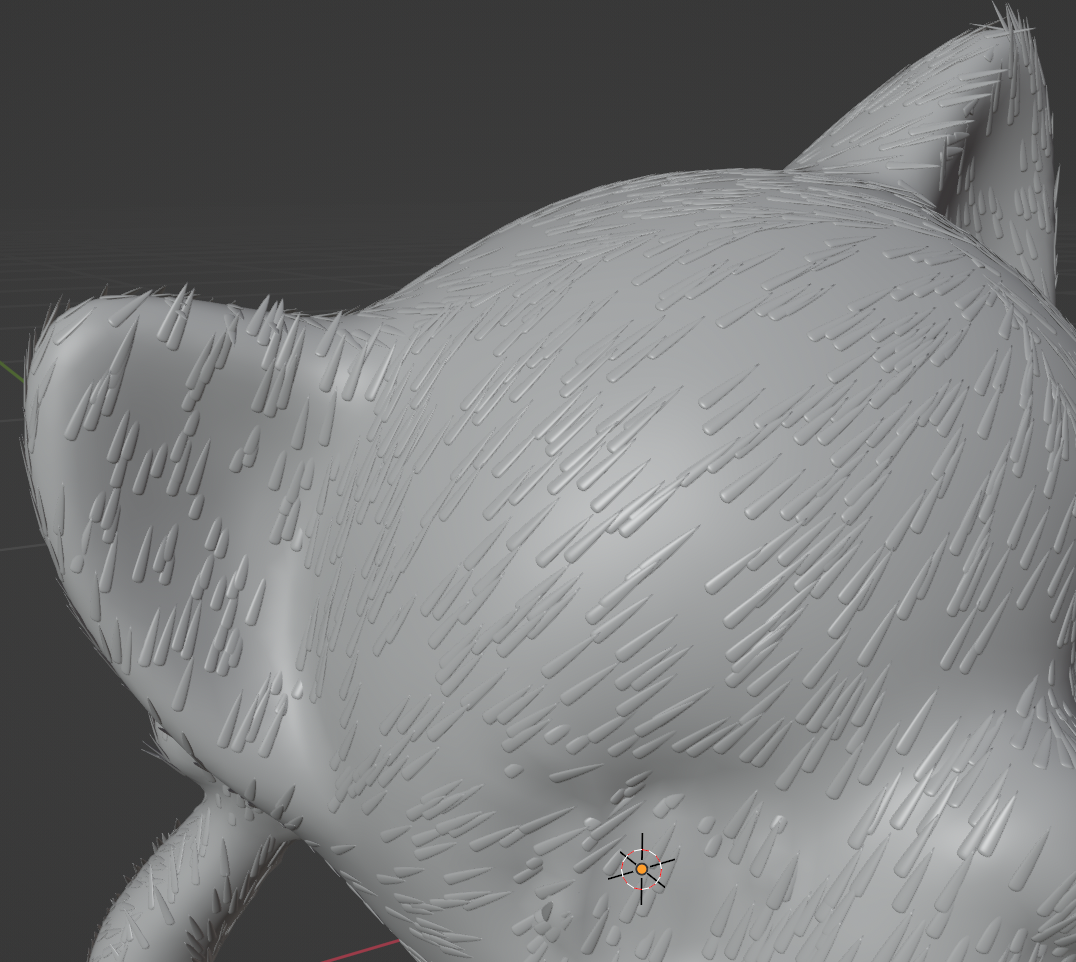
\includegraphics[width=0.7\textwidth]{images/vector_instance_adhering.png}
        \caption{Now our flattened arrows lie flat along the surface!}
        \label{fig:vector_instance_adhering}
    \end{figure}
    \item Currently there are too many arrows, and all the arrows are too tiny to see well. Also, the arrows are somewhat clumped. The vector field visualization would be better if the sampling rate was less than one vector per face. We \emph{could} cull arrows by randomly selecting a proportion of them and setting their lengths to zero, but this provides an uneven sampling:
    \begin{figure}[H]
        \centering
        \captionsetup{width=0.8\textwidth}
        \begin{subfigure}[b]{\textwidth}
         \centering
         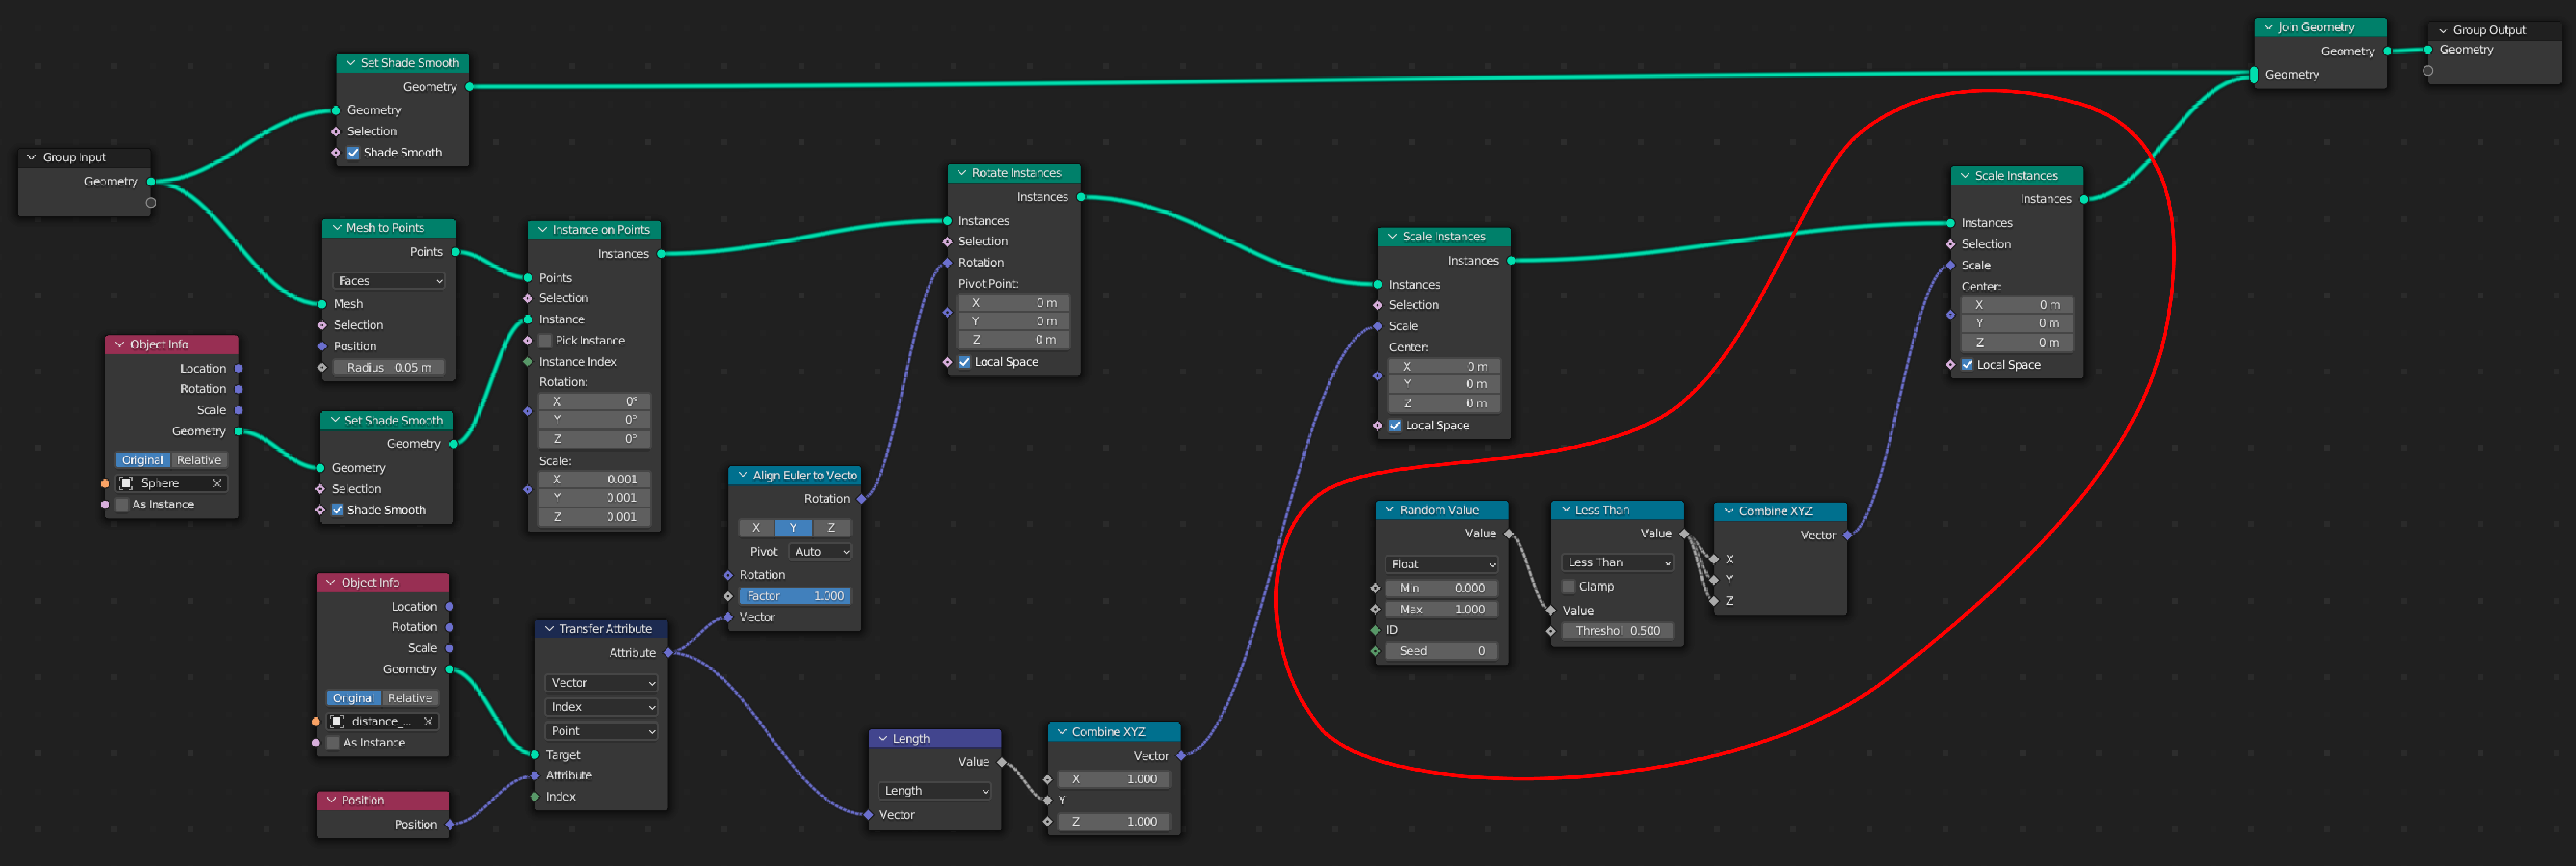
\includegraphics[width=\textwidth]{images/vector_instance_random-cull_nodes.png}
         \caption{The updated node configuration for randomly culling instances, in case you wanted to do something similar. New nodes added in this step are indicated in red.}
        \end{subfigure} \\
        \begin{subfigure}[b]{\textwidth}
         \centering
         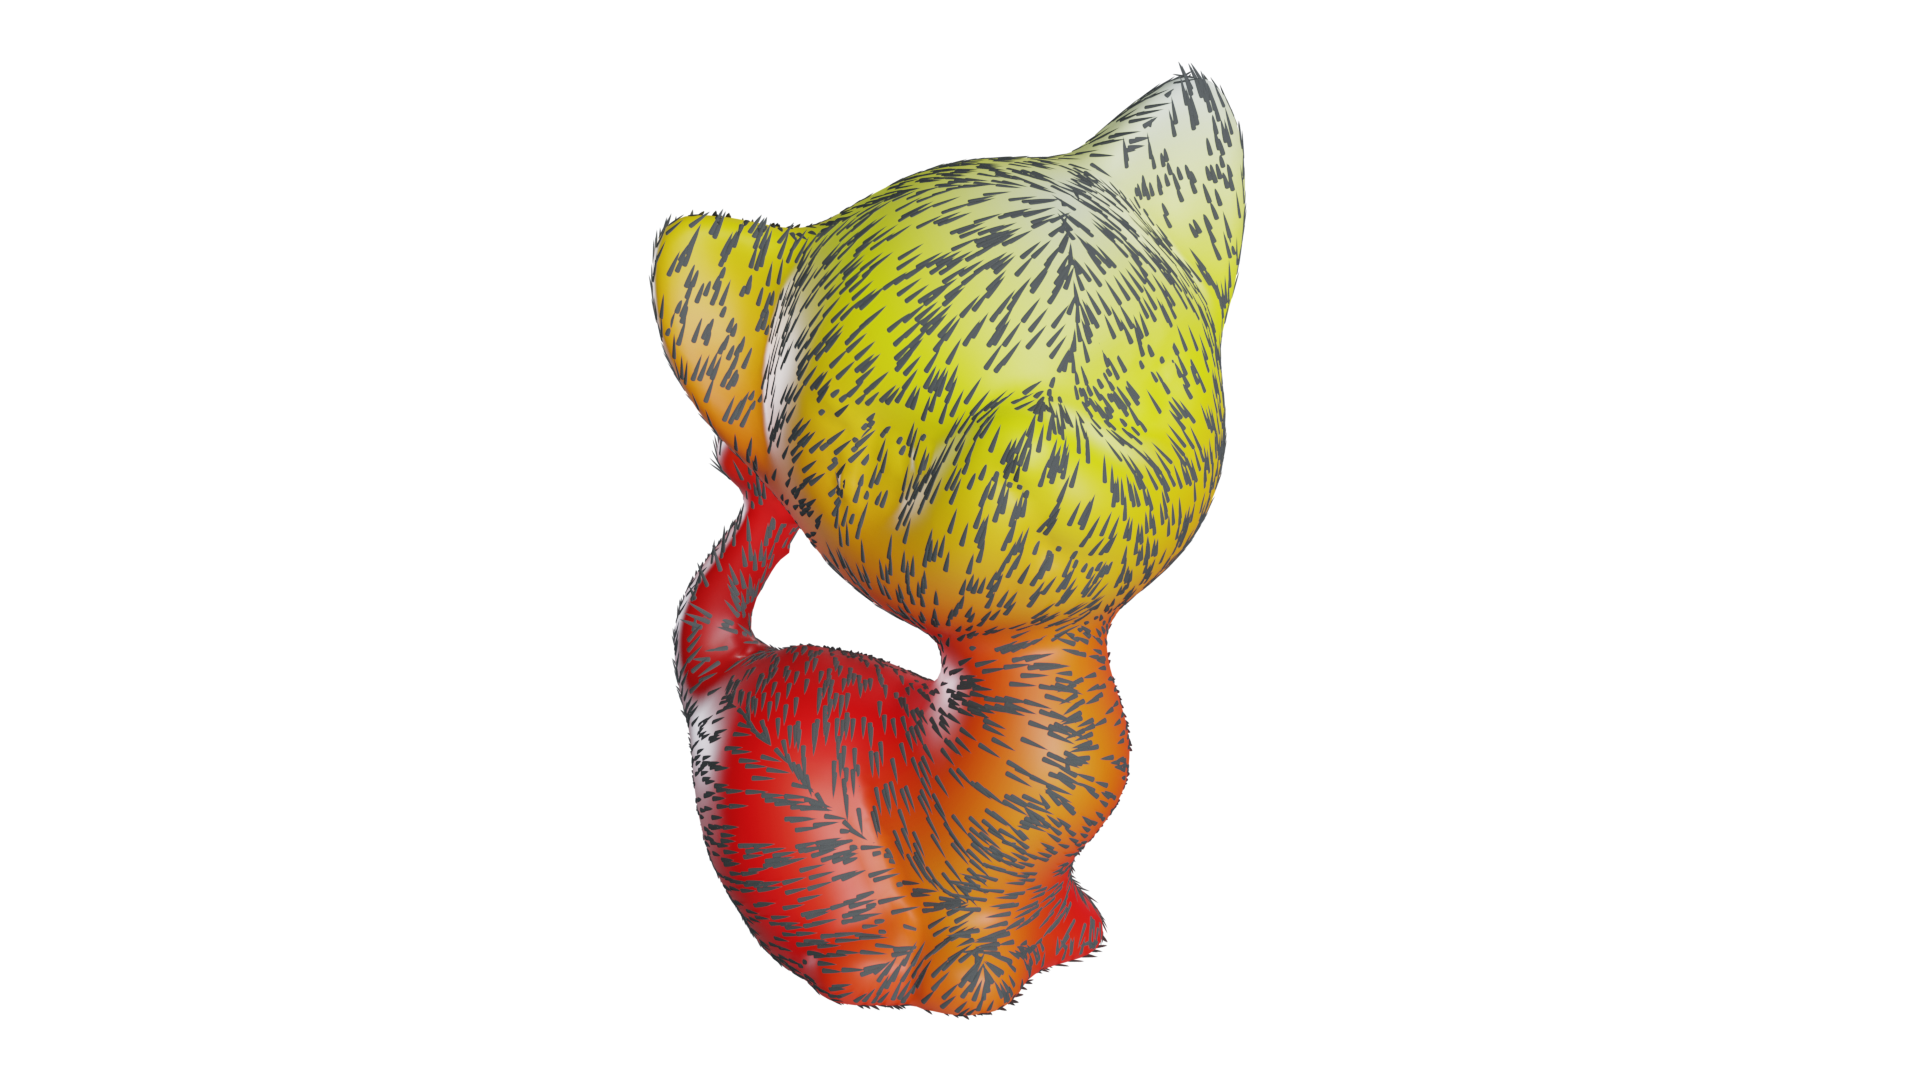
\includegraphics[width=0.8\textwidth]{images/vector_instance_random-cull.png}
         \caption{The result, which doesn't look great.}
        \end{subfigure}
        \caption{Randomly culling arrows provides an uneven sampling. Do NOT do this.}
        \label{fig:vector_instance_random-cull}
    \end{figure}
    A better method is to use something like Poisson Disk Sampling; the Vector Heat Method paper used \href{https://www.cs.ubc.ca/~rbridson/docs/bridson-siggraph07-poissondisk.pdf}{this method by Bridson}. It's easiest to implement the sampling algorithm in the code you used to generate the file containing the vector information, so probably not via Blender. As of writing this section (July 2022), I've added a \texttt{PoissonDiskSampler} class to \href{https://geometry-central.net/}{geometry-central}, though implementations of Poisson disk sampling for surface meshes also exist in \href{https://www.meshlab.net/}{MeshLab}, among other software.
    \item Now I've implemented the Poisson disk sampling algorithm mentioned in the previous step, and re-written the OBJ file containing rotation information. Specifically, I've written one OBJ file that contains the locations at which vectors are sampled (as vertex positions), and a second OBJ file that contains the corresponding vectors at those sampled locations (also as vertex positions.) Ideally I would have stored the vectors as vertex normals within the first OBJ file, but I had trouble getting Blender to recognize them. Now our vector field looks like this:
    \begin{figure}[H]
        \centering
        \captionsetup{width=0.8\textwidth}
        \begin{subfigure}[b]{\textwidth}
         \centering
         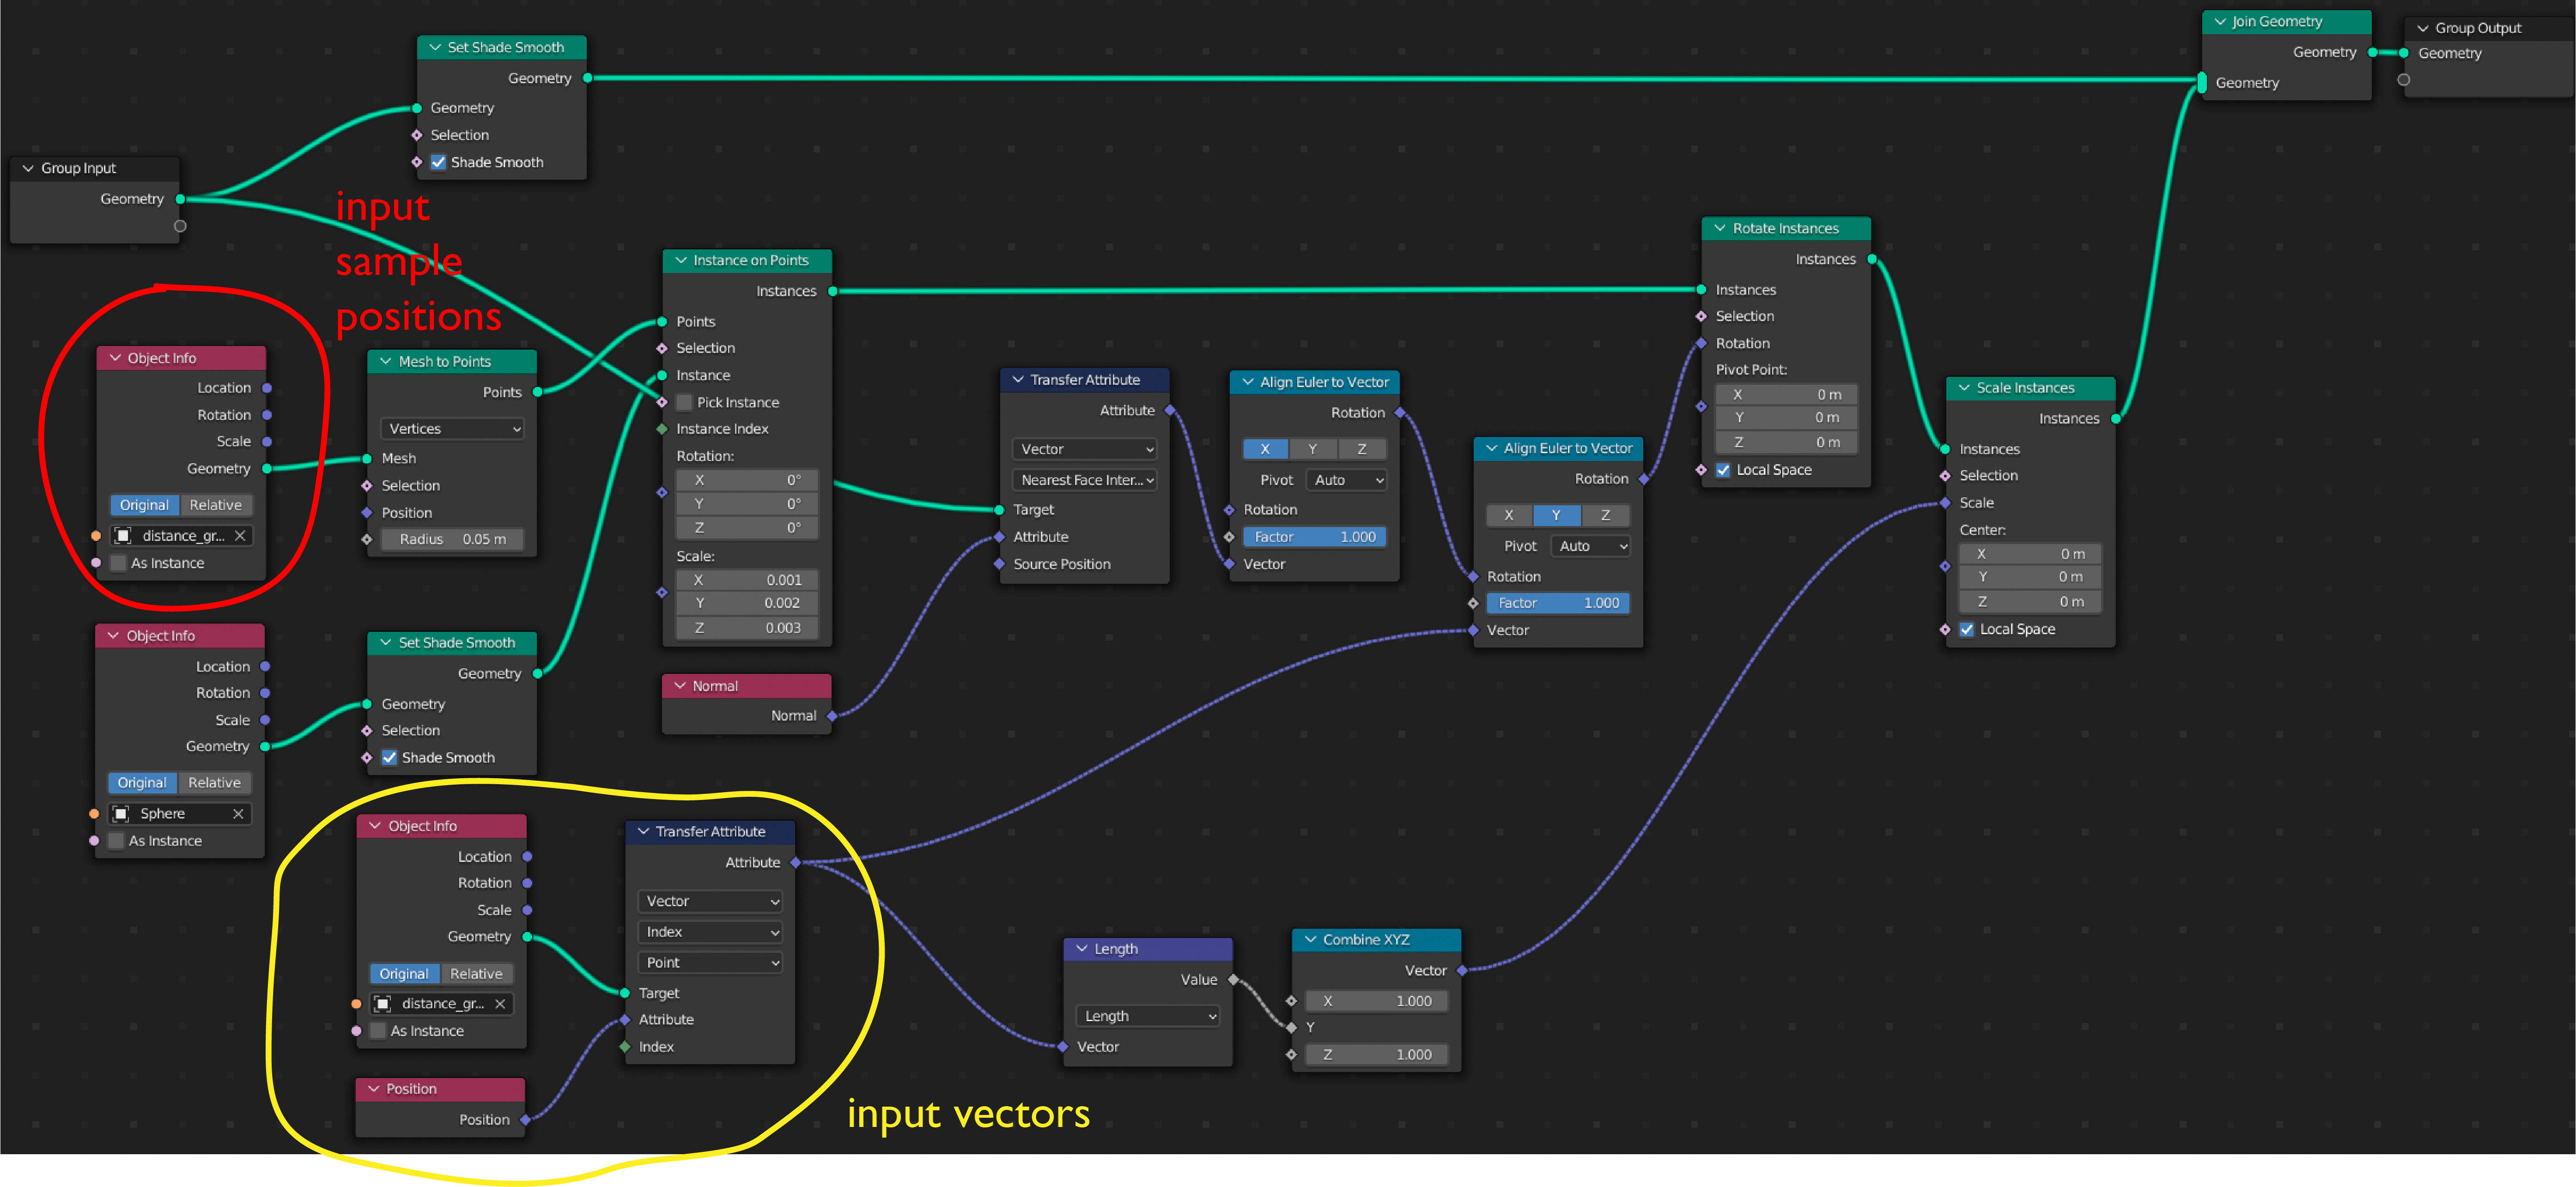
\includegraphics[width=\textwidth]{images/vector_instance_sampled-nodes.png}
         \caption{The updated node configuration.}
        \end{subfigure} \\
        \begin{subfigure}[b]{\textwidth}
         \centering
         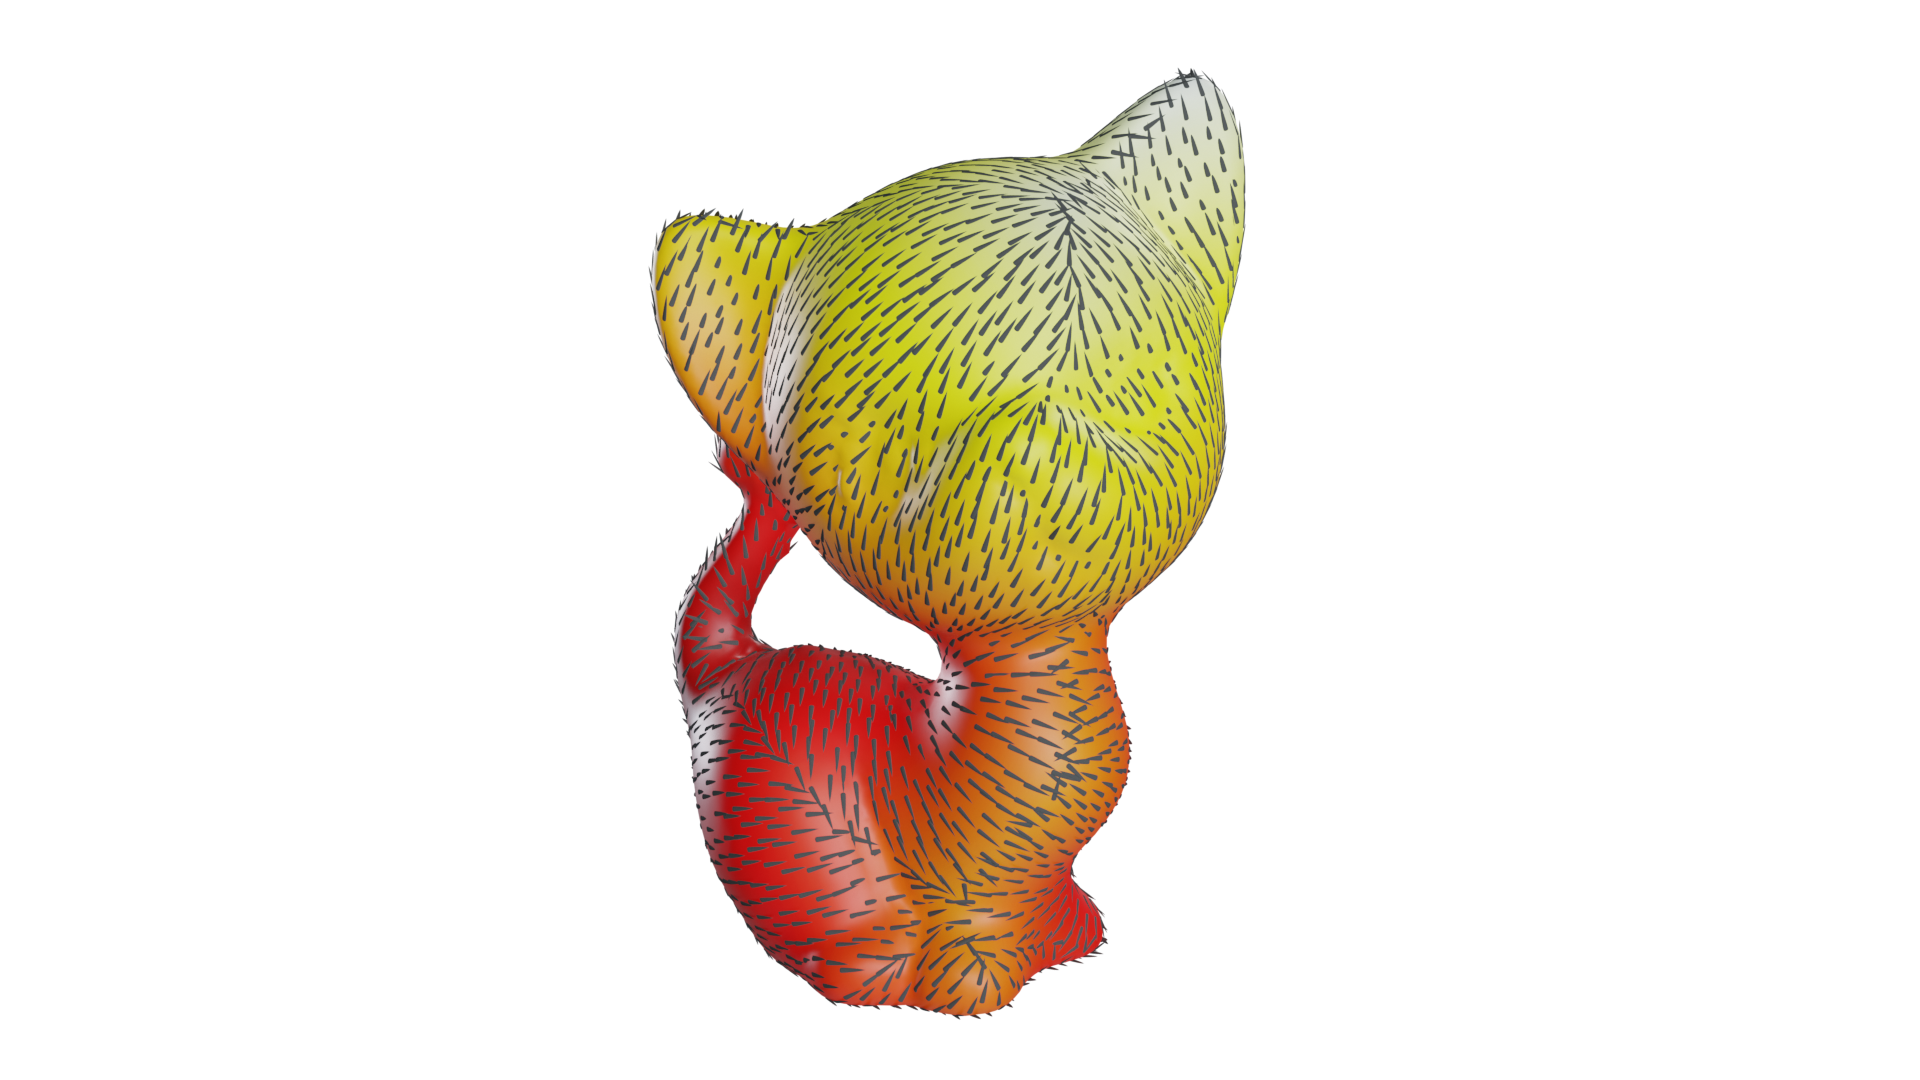
\includegraphics[width=0.8\textwidth]{images/vector_instance_poisson-sampled.png}
         \caption{}
        \end{subfigure}
        \caption{A Poisson-sampled surface -- much better!}
        \label{fig:vector_instance_poisson-sampled}
    \end{figure}
    \item As an optional visual tweak, you may want to adjust the darkness of your arrows to be inversely proportional to the darkness of the underlying mesh, for optimal contrast between the arrows and the surface mesh.
    
    One way to do this is save yet another file containing the scalar function evaluated at each vector of your vector field, and import this data via nodes. Again, this may be a non-optimal way to import attribute data; scripting may be a much better ``one-shot'' way to import data (you could write a Python script that reads any data you'd like, in any way you'd like, from any file(s)), but so far this method has been reasonably efficient for me.
    
    The following commands assume Blender version 3.2.1 or higher. Go to the Geometry Shading editor where you have all the geometry nodes for your vector field set up. Add a \obj{Store Named Attribute} node. Feed the last of nodes controlling the instanced geometry into the ``Value'' field of \obj{Store Named Attribute}. Input the scalar data you want to store on the instances into \obj{Store Named Attribute}, and set the attribute domain to ``Instance'', and set the data type appropriately (in this case, float.) Give a name to your attribute; here I've just named it ``col''. Node configurations are shown in Fig.~\ref{fig:instances_attributes_node}.
    \begin{figure}[H]
        \centering
        \captionsetup{width=0.8\textwidth}
        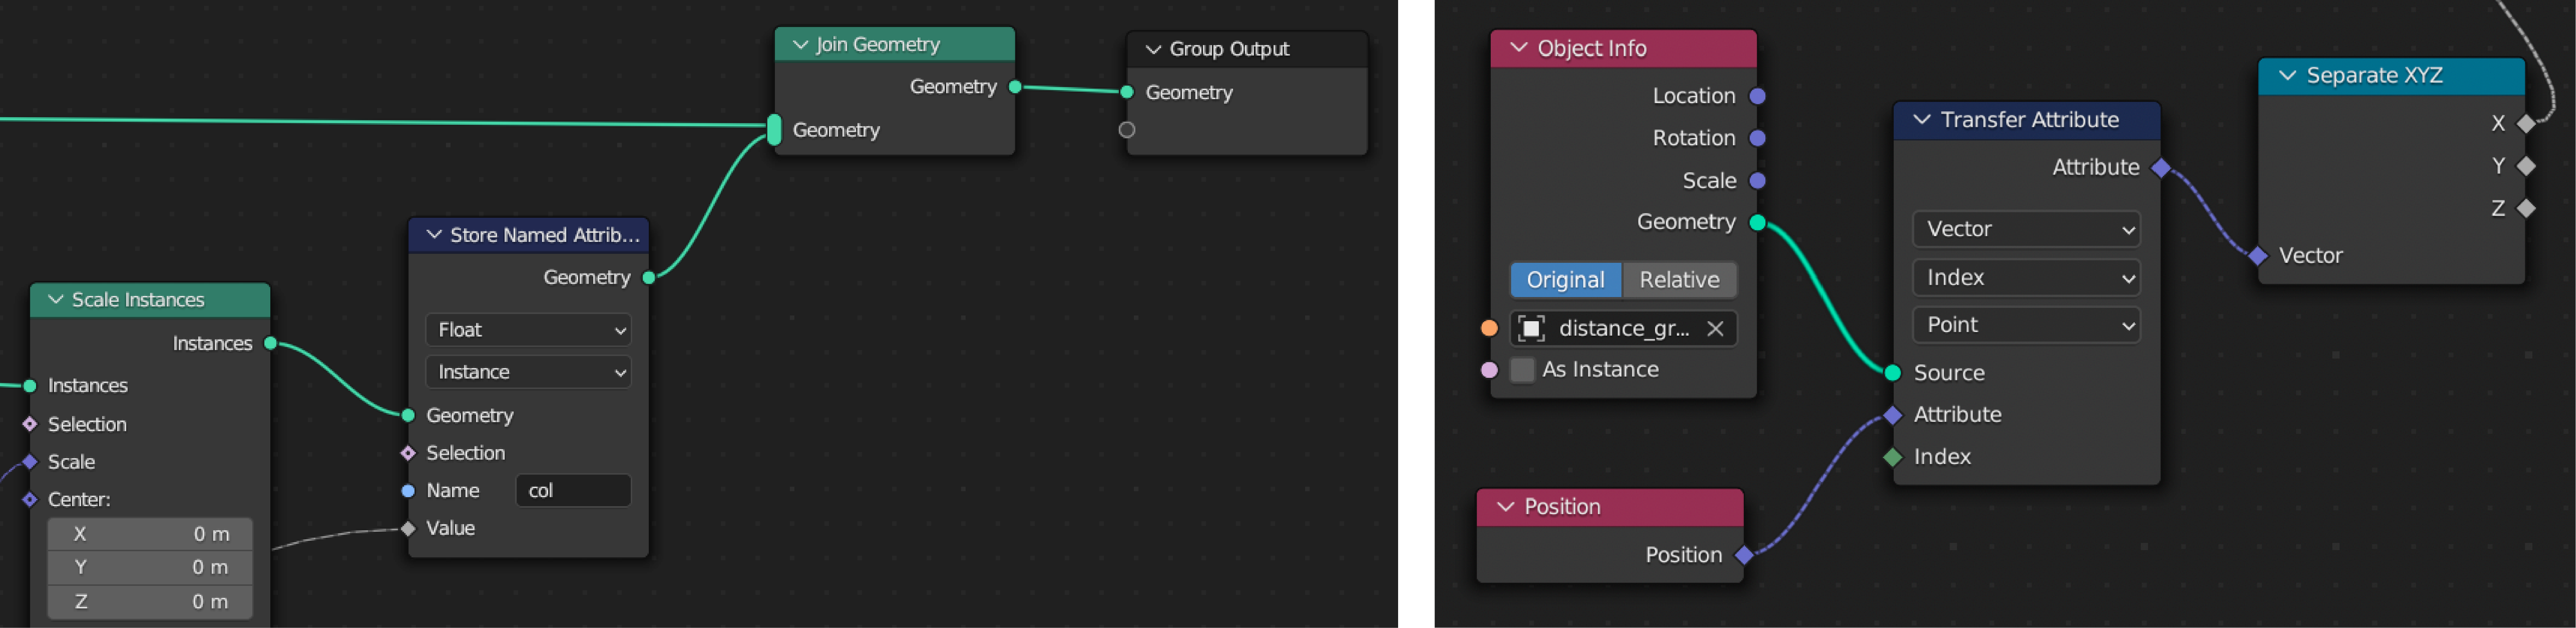
\includegraphics[width=0.9\textwidth]{images/instances_attributes_node_v2.png}
        \caption{Left: Adding the nodes that will allow us to define an attribute on instanced geometry. Right: The nodes used to extract the scalar field values at the instance samples; in this example, I've stored the values as the x-coordinate of vertex positions in a separate OBJ file. \textit{Note:} In newer versions of Blender (3.4+), the function of the \obj{Transfer Attribute} node has been incorporated into the \obj{Sample Index} node instead.}
        \label{fig:instances_attributes_node}
    \end{figure}
    
    Go to the Shading editor and select the arrow object used for instancing. Add an \obj{Attribute} node, and specify which attribute you want to access -- in this example, I called the attribute ``col''. Hook this up to the same colormap you used to visualize the scalar function on the surface -- now at each instance, we have the color of the mesh directly underneath the instance. We want to use this color to determine the gray level that optimally contrasts with this color. This corresponds to computing the relative luminance (contrast ratio) between colors. 
    
    Instead of computing luminance ourselves, we can simply use the \obj{RGB to BW} node. I've added nodes to compute $(1 - \text{luminance})$, and also re-mapped the range so that there's less white in this particular example. On the other hand, it's probably easier to use an \obj{Invert} node instead. The updated Shader node configuration is shown in Figure~\ref{fig:color_instances_luminance}. The arrows will be rendered in shades of gray, using a lighter shade of gray in areas with darker colors, and vice versa. 
    \begin{figure}[H]
        \centering
        \captionsetup{width=0.8\textwidth}
        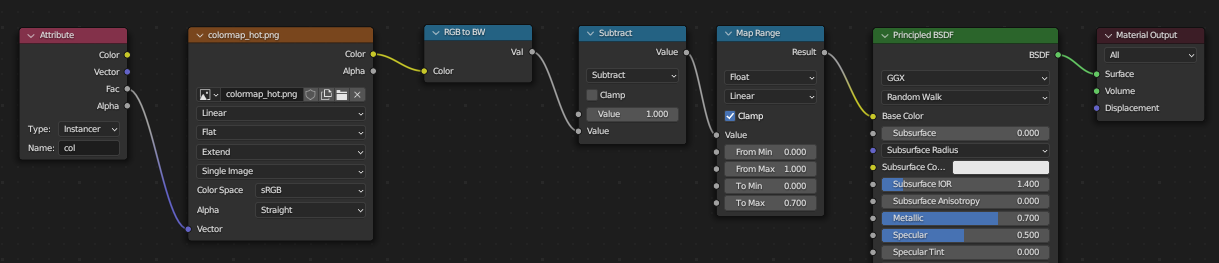
\includegraphics[width=\textwidth]{images/color_instances_luminance_nodes_v2.png}
        \caption{The updated node configuration in the Shader editor. Maybe a better way to do the inverse mapping (instead of the math nodes I used), is to simply use an \obj{Invert} node.}
        \label{fig:color_instances_luminance}
    \end{figure}
    \item Here's the final render. Throughout this example, I've prevented the arrows from having shadows rendered on them because I find them distracting in this particular example (\menu{Properties > Object Properties > Visibility > Ray Visibility} and uncheck ``Shadow''.) % In this particular render, I've also upped the saturation and brightness of the colors because the colors looked a bit dark before, by setting the S and V values of the mesh colors, in HSV representation, to 1.0. On the other hand, this might mess with the perceptual effectiveness of the colormap, so... maybe don't do this.
    \begin{figure}[H]
        \centering
        \captionsetup{width=0.8\textwidth}
        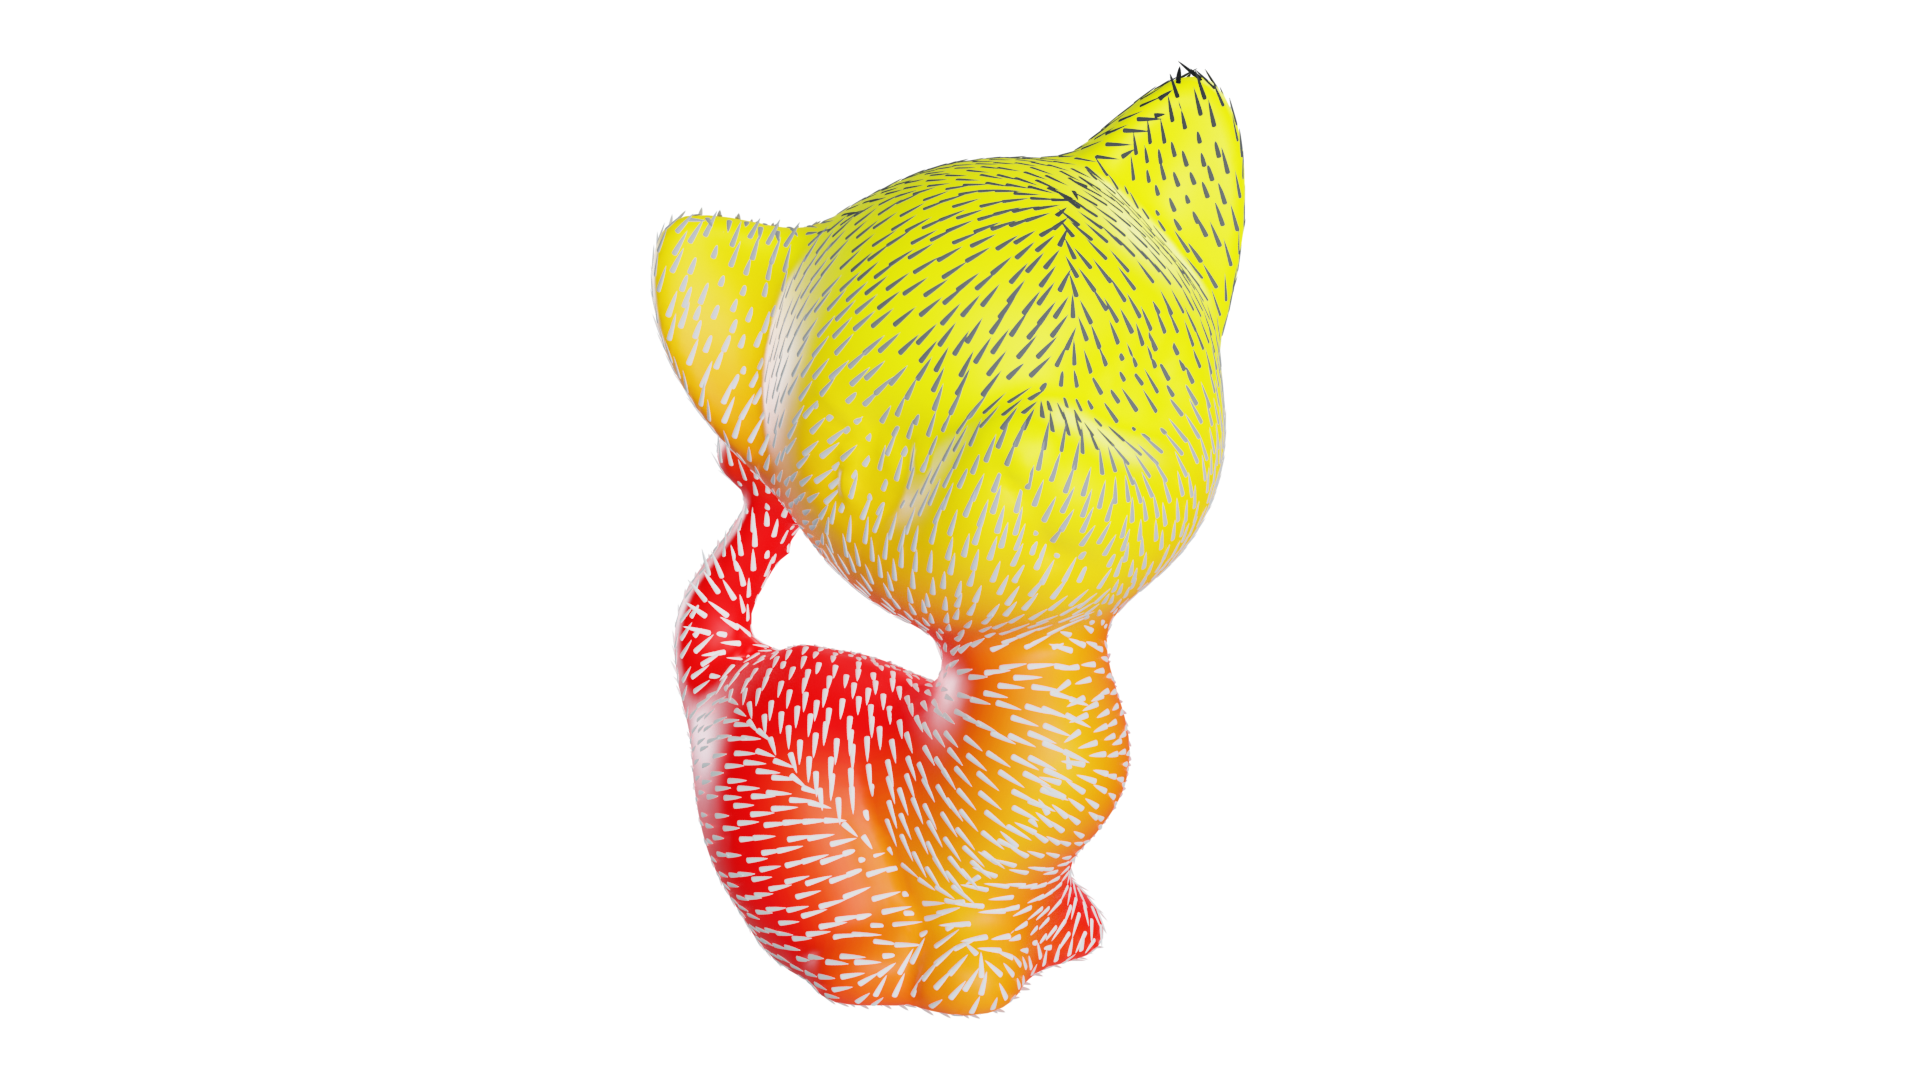
\includegraphics[width=0.9\textwidth]{images/vector_field_final_render.png}
        \caption{The ``final'' render. I'd personally still want to tweak the color gradient of the arrows, since the white arrows against the yellow portion of the surface are a bit hard to see. We would probably still want to make some tweaks to make the render look even better; see the sections on materials, lighting, and Section~\ref{sec:Prettification} for more tips.}
    \end{figure}
\end{enumerate}

\subsection{Streamlines}
\textbf{TODO}:

\section{Rendering data with more than 3 dimensions}
\textbf{TODO}: Probably easiest to do by using more than one file as input (and combining inputs appropriately), or co-opting other data-types in the same file. Or perhaps a Python script; see answers like \href{https://blender.stackexchange.com/a/118494}{this one.}

\section{Rendering curves}
\subsection{Basics}
\begin{enumerate}
    \item OBJ files can contain ``line'' elements. A line element is specified in an OBJ file with a line starting with the letter ``l'', followed by a sequence of vertex indices which build a polyline. 
    \item Load your OBJ into Blender. We will convert the polyline to a \obj{Curve} object, for which there are nice rendering options in Blender. To convert to a \obj{Curve}, select \menu{Object > Convert to > Curve}.
    \item Currently the curve will have zero width. To thicken the curve, go to \menu{Properties > Object Data Properties} (\includesvg[height=1em]{images/curve_data.svg} icon in the right menu panel.) Go the \directory{Geometry / Bevel} within this tab, and up the ``Depth'' value. You may need to also up the ``Resolution'' value to maintain a smooth appearance. If this doesn't have an effect, make sure that \directory{Shape / Fill Mode} is set to ``Full''.
    \item By default, the profile of the curve is circular.
    \item You can set the material properties of the \obj{Curve} like you would any other object, in \menu{Properties > Material Properties} (the \inlinepic{images/material-properties-icon.png} icon in the right menu panel.)
\end{enumerate}

\begin{figure}[H]
    \centering
    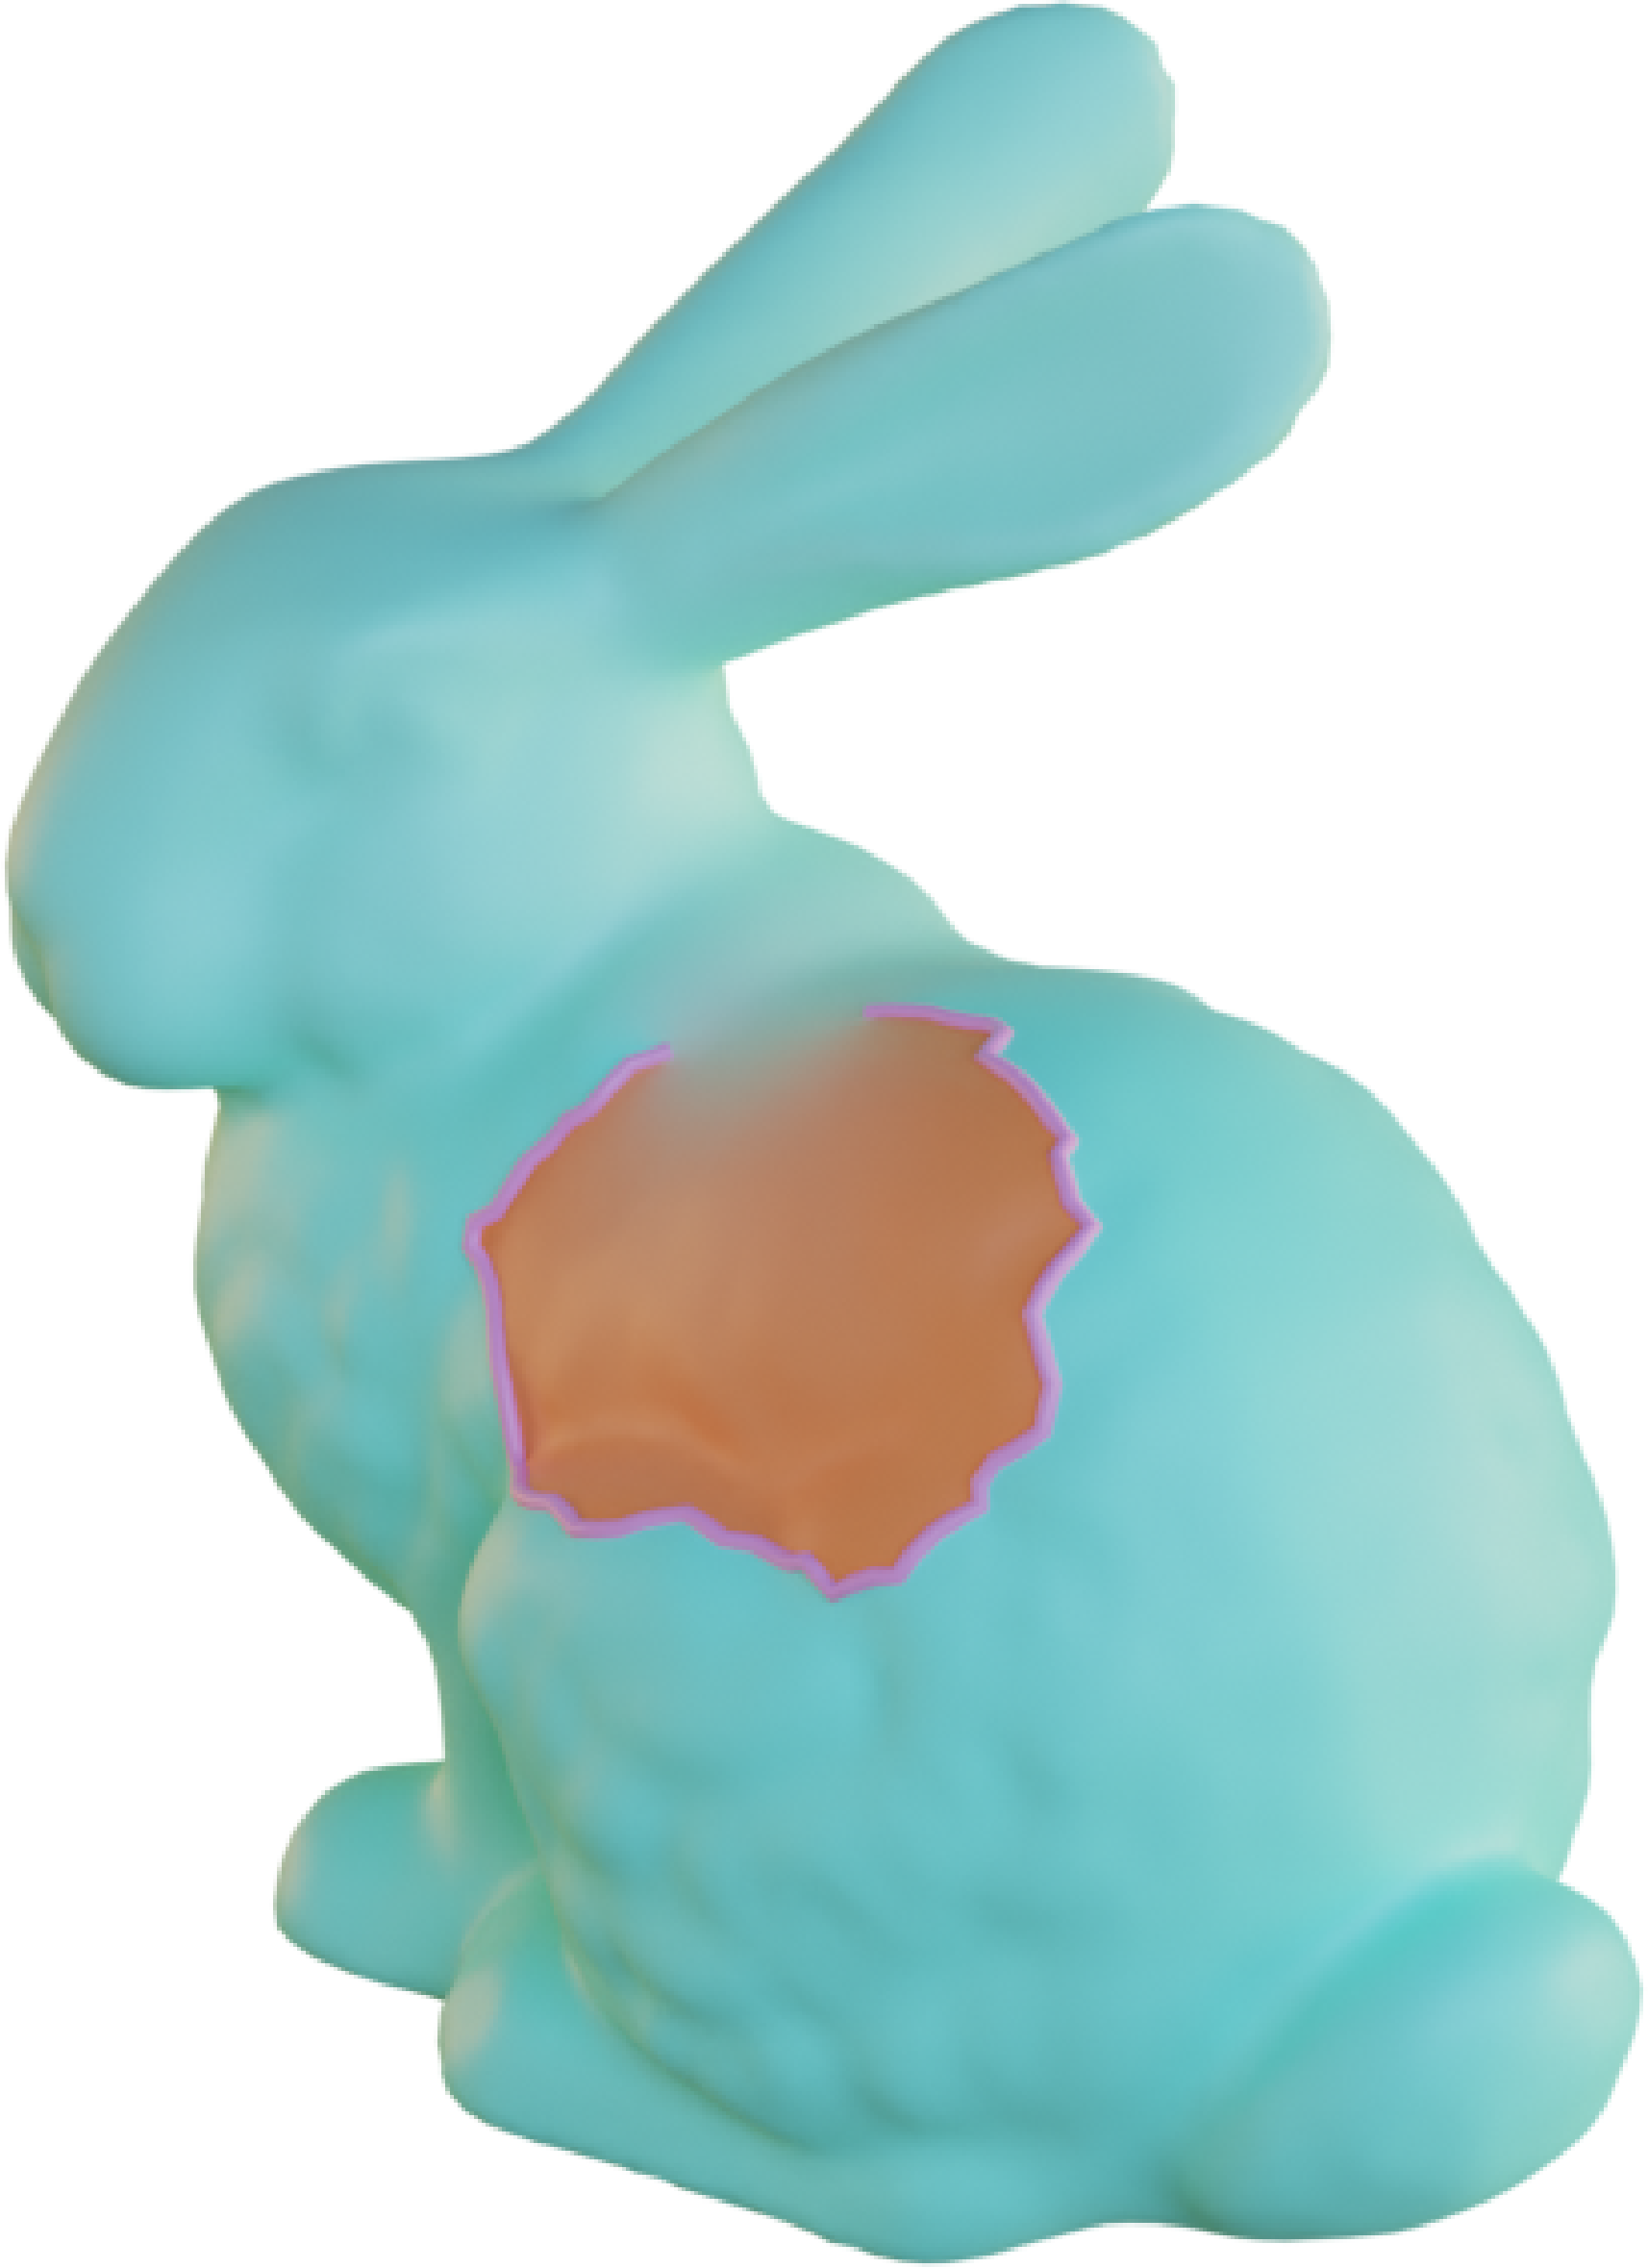
\includegraphics[width=0.3\textwidth]{images/bunny-with-round-curve.png}
    \caption{A bunny mesh with a round purple-colored \obj{Curve} on it.}
    \label{fig:curve}
\end{figure}

Additional options:
\begin{itemize}
    \item For more complex cross-sections, you can use a more complicated bevel (in \menu{Properties > Object Data Properties > Geometry > Bevel}) or using a \obj{Bevel} object (I have never tried the latter.)
    \item To prevent the curves from casting a shadow on other objects, you must have selected``Cycles'' as the render engine (Section~\ref{subsec:eevee_vs_cycles}). Make sure the curve object is selected in the viewport, then go to \menu{Properties > Object properties} \inlinepic{images/object-properties-icon.png} and \directory{Visibility / Ray visibility} and uncheck the ``Shadow'' box. You might want this feature, for example, if you're rendering curves that lie along a surface, and you want the curves to have volume but not cast distracting shadows on the surface.
\end{itemize}

% As discussed in Section~\ref{sec:RenderingScalarDataOnSurfaceMeshes}, you can store data in UV maps to use as rendering info. Figure~\ref{fig:colored_curve} is an example of using UV coordinates to color the vertices of the curve, and Figure~\ref{fig:alpha_curve} is an example of using UV coordinates to control the transparency (alpha values) of the curve. Although the curve is beveled, the coloring is done per vertex of the underlying control curve. (TODO: I have yet to figure out how exactly the UV values map on to elements of the curve; can't tell if it is doing per vertex, per halfedge, etc. I actually have no idea what it's doing.)
% \begin{figure}[H]
%     \centering
%     \captionsetup{width=0.8\textwidth}
%     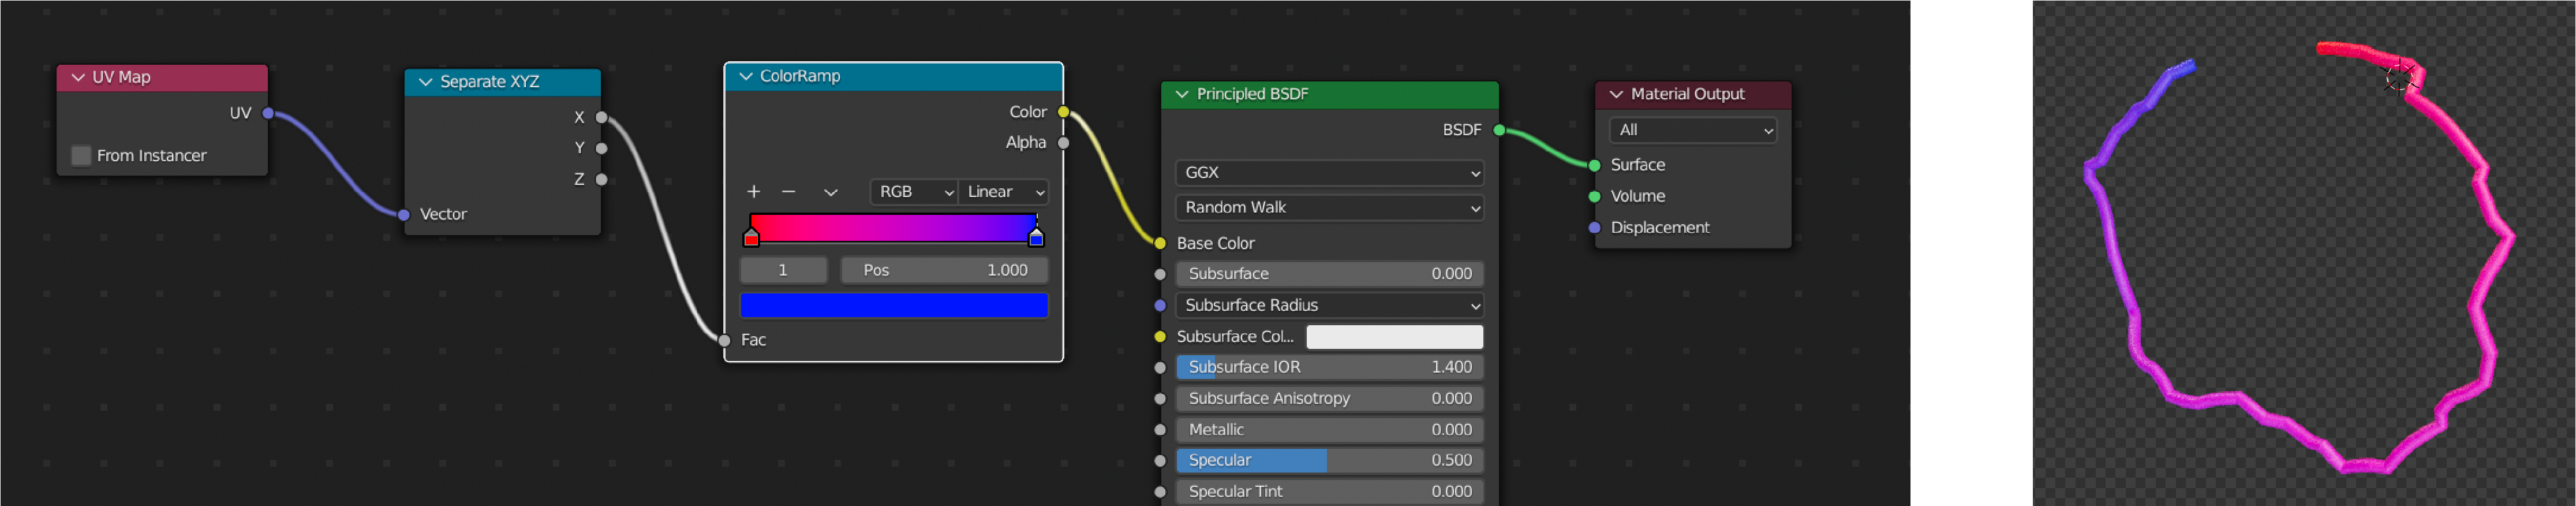
\includegraphics[width=0.9\textwidth]{images/color-curve.png}
%     \caption{Coloring the control vertices of a beveled curve.}
%     \label{fig:colored_curve}
% \end{figure}

% \begin{figure}[H]
%     \centering
%     \captionsetup{width=0.8\textwidth}
%     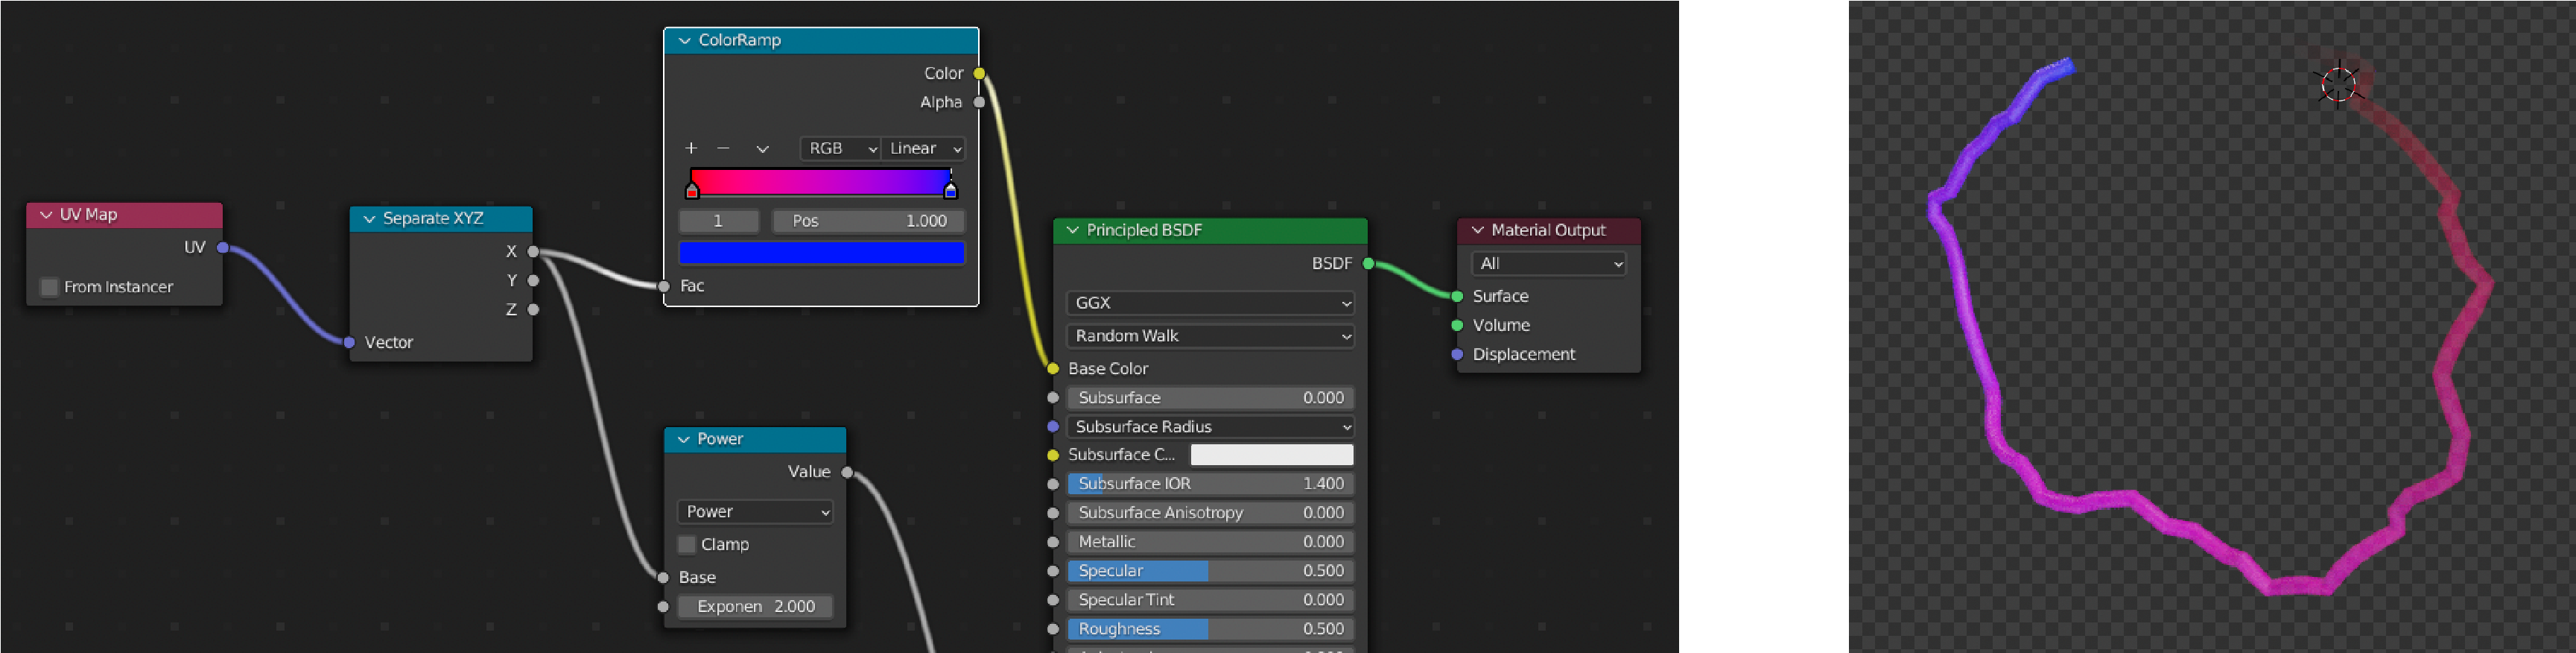
\includegraphics[width=0.9\textwidth]{images/alpha-curve.png}
%     \caption{Additionally setting the alpha values of vertices of a beveled curve via UV map. I added a \obj{Math} node (set to ``Power'') to remap the alpha values to something more visually appealing.}
%     \label{fig:alpha_curve}
% \end{figure}

\subsection{Making curves lie flat against a surface}
{\bf TODO: This section under heavy construction --- not safe for reading. I've found a way to do this using Geometry Nodes, but it's still not perfect.}
If you're rendering curves that lie along a surface and want the curves to lie flat on the surface, I have no idea how to do this. I tried for ages fiddling with the Bevel options and constructing my own Bevel (which is an option in Blender 3.0+), but it seems like the beveled curve will always have thickness. I suppose a solution is to construct your own polygon strip from the curve, and export that as a mesh.

\subsection{Assigning UV coordinates}
{\bf TODO: This section under heavy construction --- not safe for reading}
Unfortunately, Blender doesn't have a way to store info along a Curve -- you're only able to store UV coordinates if the Curve has been converted into Mesh, from which there doesn't appear to be a way to determine the coordinates corresponding to the control points of the original curve. This stinks, because a lot of the time we want to store per-vertex or per-segment attributes for a Curve, and this prevents us from doing so.

What's kind of silly is that Curves \emph{do} have UV maps in Blender -- it's just that there's no way to change it. The auto-generated UV map for a Curve divides the UV space more-or-less linearly between the points of the curve. So for example, you can use these UV coordinates to render simple gradients that interpolate from 0 at one end to 1 at the other end of the curve:
\begin{figure}[H]
    \centering
    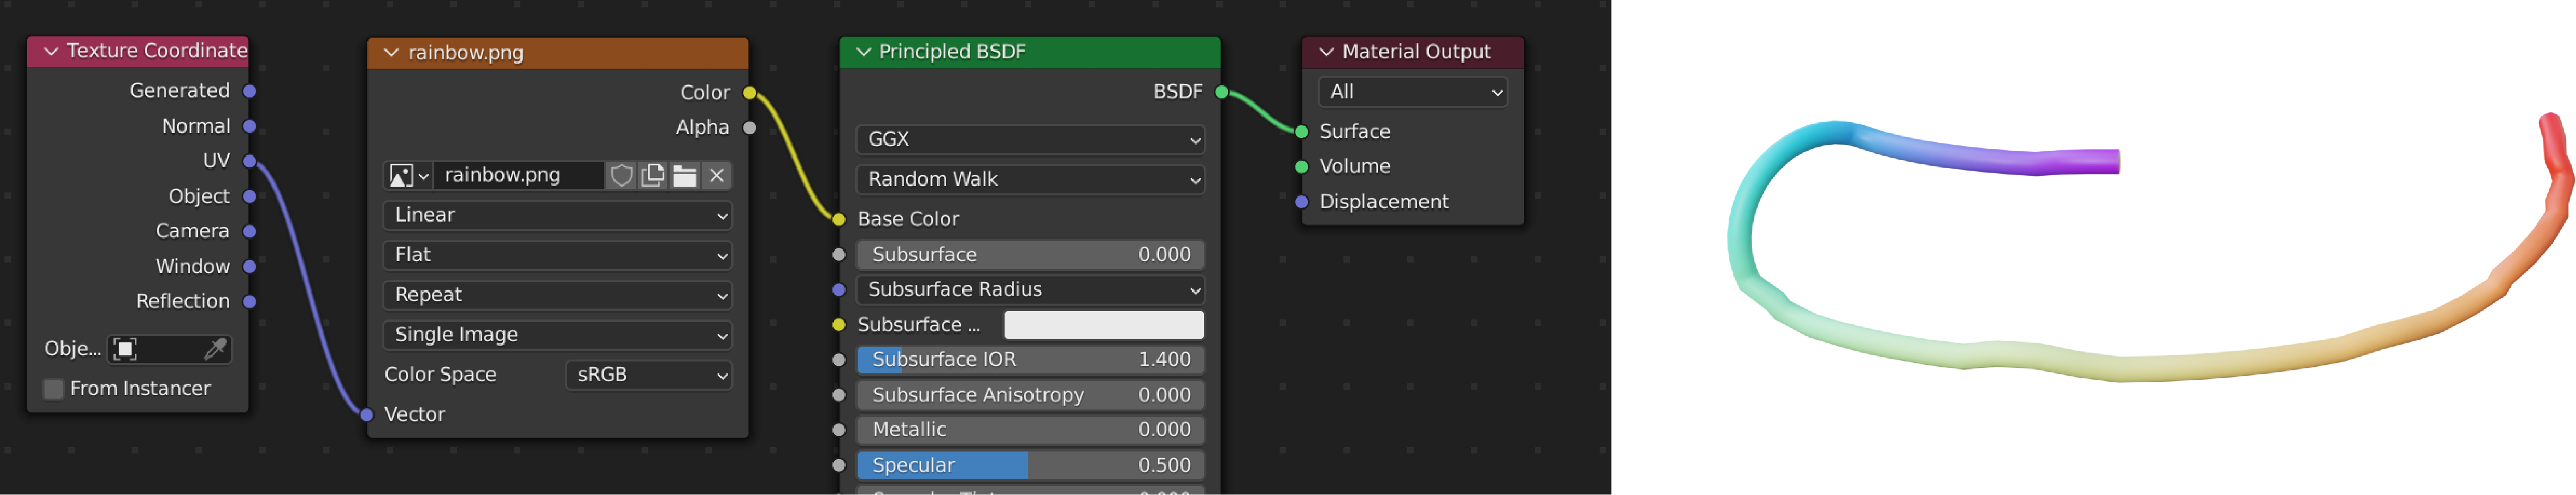
\includegraphics[width=0.9\textwidth]{images/curve_auto_uv.png}
    \caption{Using Blender's auto-generated UV coordinates to make a simple color gradient along a curve.}
    \label{fig:curve_auto_uv}
\end{figure}

Therefore one possible workaround is to take advantage of these built-in UV coordinates to map a custom texture onto the Curve:
\begin{enumerate}
    \item Parameterize your curve onto $[0,1]$. Create an image texture encoding the values of your function at the corresponding $x$ location of the image.
    \item Load in this image texture; use the built-in UV coordinates to index the texture; feed the values into the shader.
\end{enumerate}

More specifically, the auto-generated UV map maps to a square. What this means is that the UV coordinates are the result of distributing UV space *equally* among segments; segments are demarcated by edge loops in the beveled curve. Edge loops are displayed in Figure~\ref{fig:curve_edge_loops}. Within each segment, UV space is distributed approximately *linearly* (up to some stretching induced by the beveling.) This is different than distributing UV space linearly along the whole curve; if you were to assign a uniform texture, you would see that the mapped texture would appear squashed on shorter segments. So you have to keep this in mind, depending on how you're trying to render your curve.
\begin{figure}[H]
    \centering
    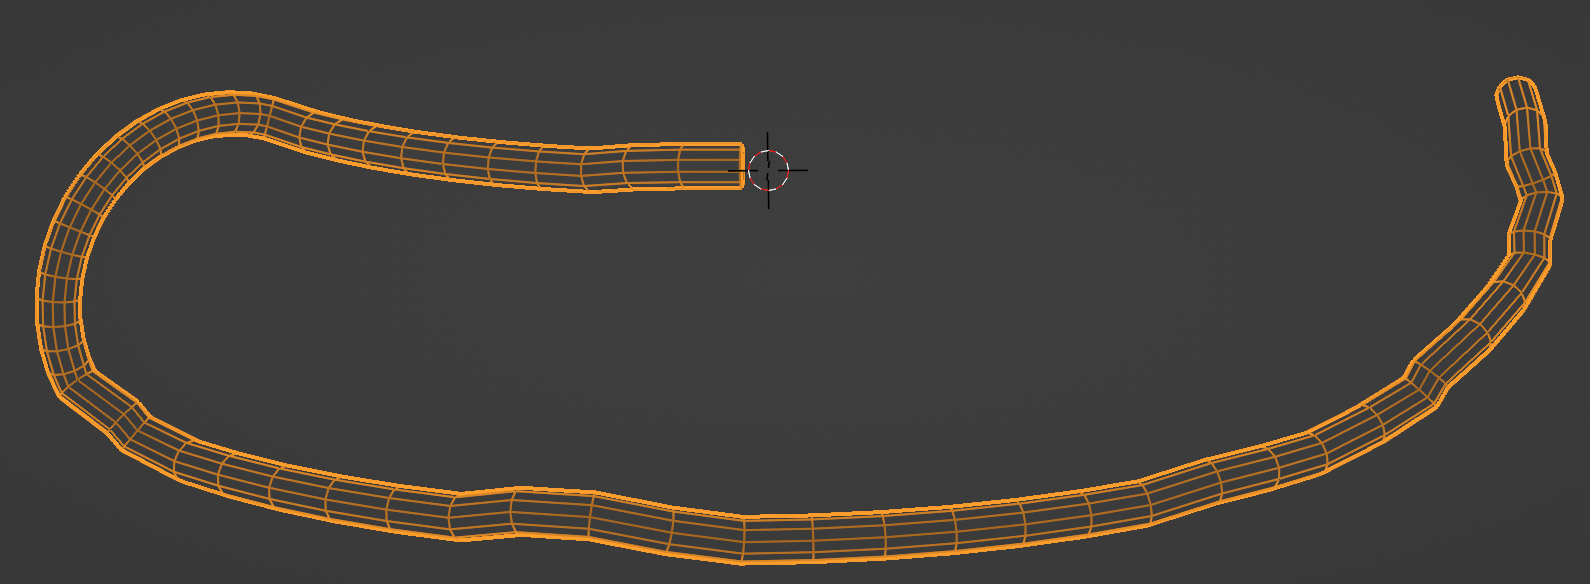
\includegraphics[width=0.5\textwidth]{images/curve_edge_loops.png}
    \caption{The edge loops on a beveled Curve.}
    \label{fig:curve_edge_loops}
\end{figure}
When you load in your curve as a line element from an OBJ file, the beveled Curve that results will have one edge loop for each vertex (every point in the line element.)

TODO: It appears that Blender does indeed UV map in this way, although it's doing other unexpected things...

Warning: How you bevel the Curve might also stretch the UV map in unexpected ways. I also have only worked with piecewise linear curves; I'm not sure how much changes with Bezier curves.

\section{Lighting}
\label{sec:Lighting}
First delete any default lights that come with the Blender file. The default lighting will almost certainly not be able to provide the best lighting for your scene.

\subsection{World lighting}

Typically I don't use environment (world) lighting; usually I find that adding a few area lights works better. (See Section~\ref{sec:DirectionalLighting}). But occasionally I find it useful --- especially for larger scenes that contain more than a few objects, such as the ``Planet Cow'' scenes from my \href{https://nzfeng.github.io/research/WNoDS/index.html}{talk on winding numbers} --- so here are some steps on the process.

Blender comes with a bunch of default materials and light sources. You can view these resources by navigating to the Blender application, and on Mac OS, right-clicking and selecting ``Show Package Contents''. The directory \directory{Contents / Resources / [version] / datafiles / studiolights / world} contains some nice default lights that will illuminate the scene from all angles. In Linux, you also navigate to where your Blender application is located, and go to \directory{[version] / datafiles / studiolights}.



\begin{enumerate}
\item Enter the Shading editor (see Figure~\ref{fig:shading_tab}.) In the upper left corner of the Shader editor, select ``World'' data from the drop-down menu:
\begin{figure}[H]
    \centering
    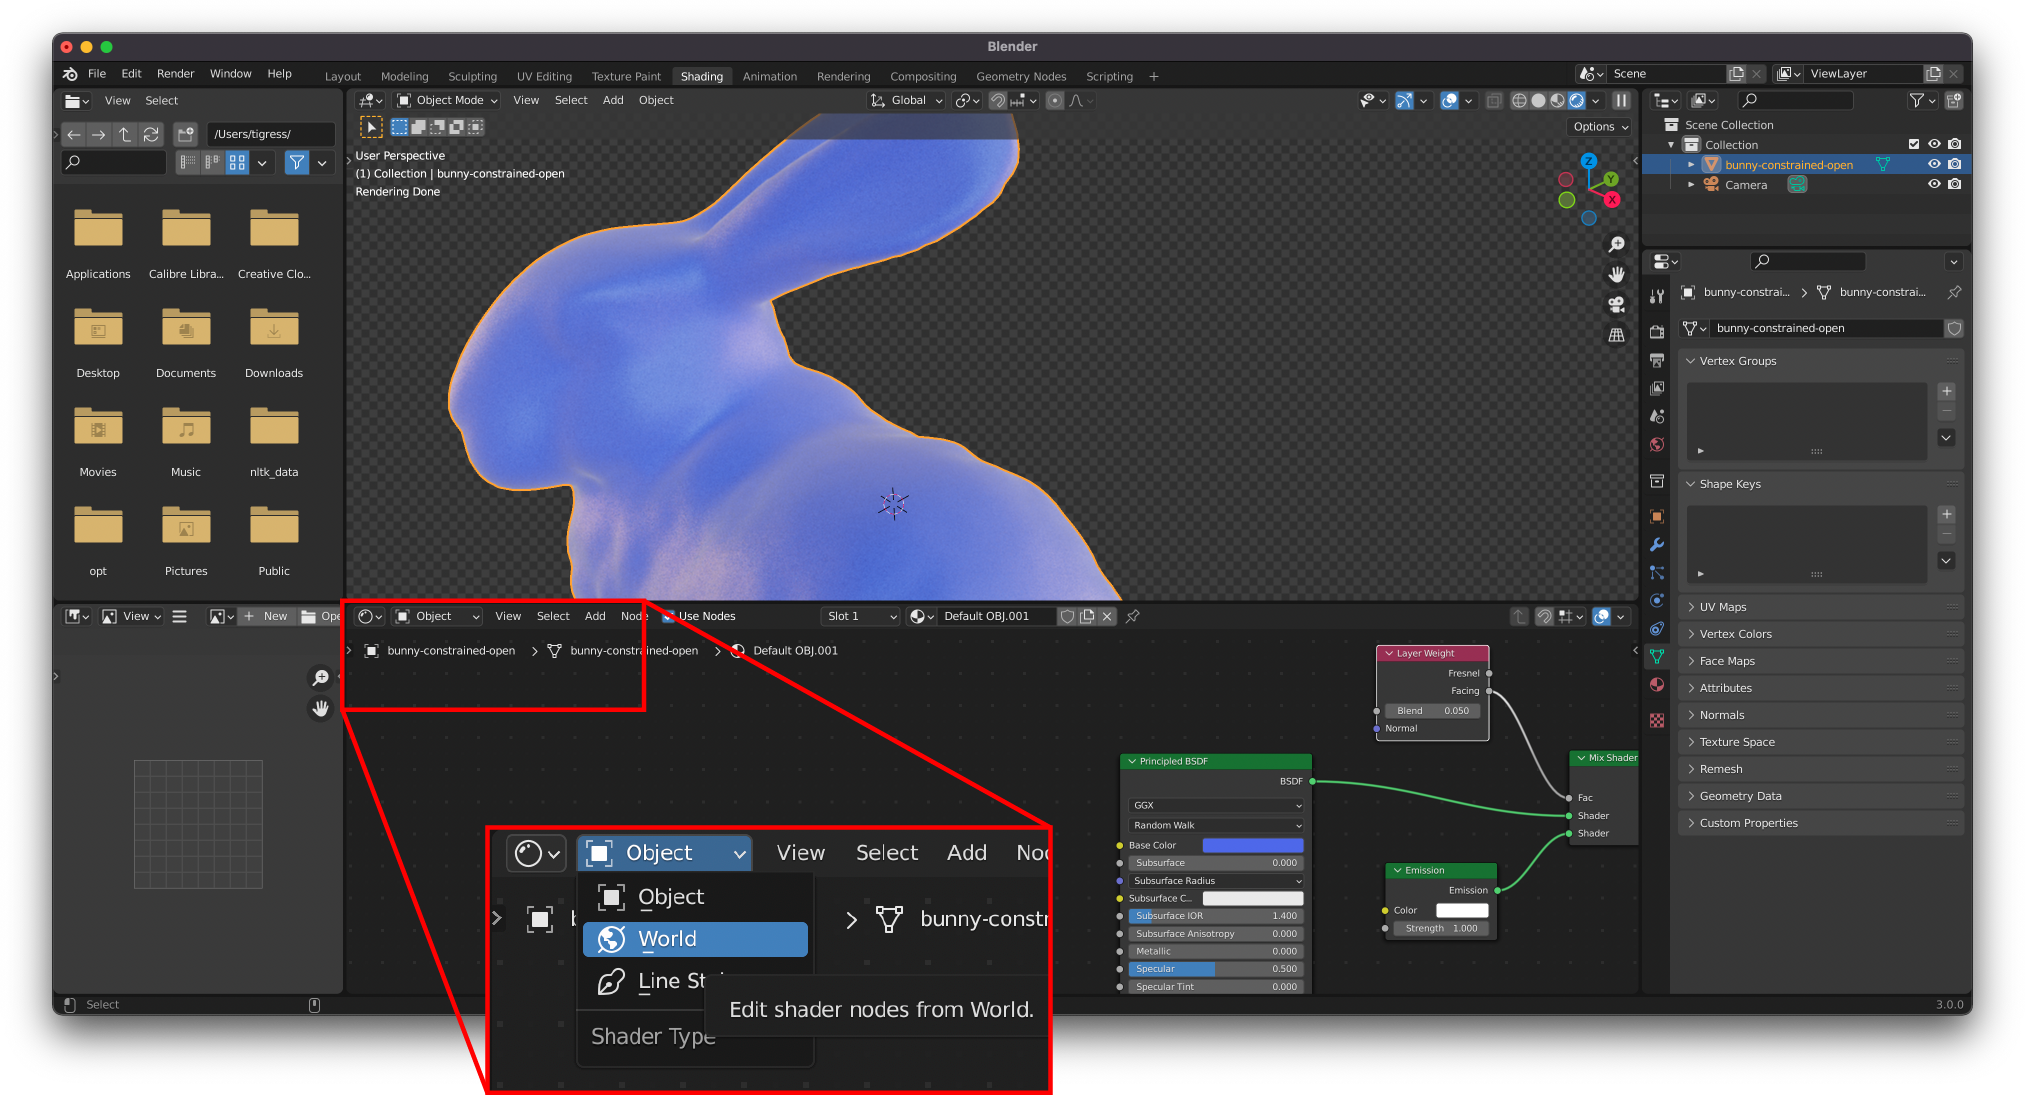
\includegraphics[width=0.8\textwidth]{images/world-lighting-nav.png}
    \caption{Navigating to world lighting in the Shading editor.}
    \label{fig:world-lighting-nav}
\end{figure}
\item Add an \obj{Environment Texture} node and connect it to the ``Color'' input of the \obj{Background} node (see Figure~\ref{fig:world-lighting-nodes}.) The \obj{Environment Texture} node has a field for a filename: click on this field and navigate to the default lighting textures in \directory{Contents / Resources / [version] / datafiles / studiolights / world}. So far I haven't found an easy way to navigate to this directory directly from the file browser that this opens up; a solution is to have the location of the lights open in a different file browser and drag in the filepath, or save the default lights in a more accessible location (i.e. not in the Blender package contents.)
\begin{figure}[H]
    \centering
    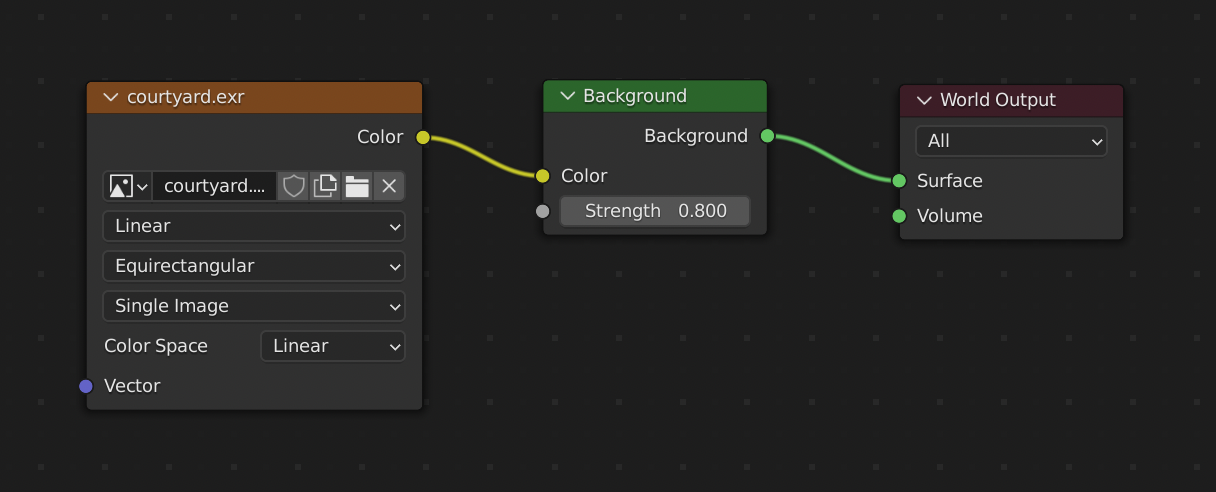
\includegraphics[width=0.6\textwidth]{images/2022-06-18_world-lighting-nodes.png}
    \caption{The nodes.}
    \label{fig:world-lighting-nodes}
\end{figure}
\item After selecting the light, you can play around with the strength and adjust it to taste. Hit \keys{F12} to get a render preview. As mentioned in Section~\ref{subsec:light_intensity}, you will probably need more light than you think, so also test out how your render will look on a white background. To do the latter, you can either paste your rendered image into a separate document, or use the Compositing editor in Blender; see Section~\ref{sec:preview_with_white_background}.
\end{enumerate}

\subsection{Directional lighting}
\label{sec:DirectionalLighting}

For scenes focused on only one or a few items, instead of adding environment lights I almost always add specific directional lights to create aesthetically-pleasing self-shadows on the object, which I find gives the object a better sense of ``3D-ness'' and ``3D placement''. 
\begin{figure}[H]
    \centering
    \captionsetup{width=0.8\textwidth}
    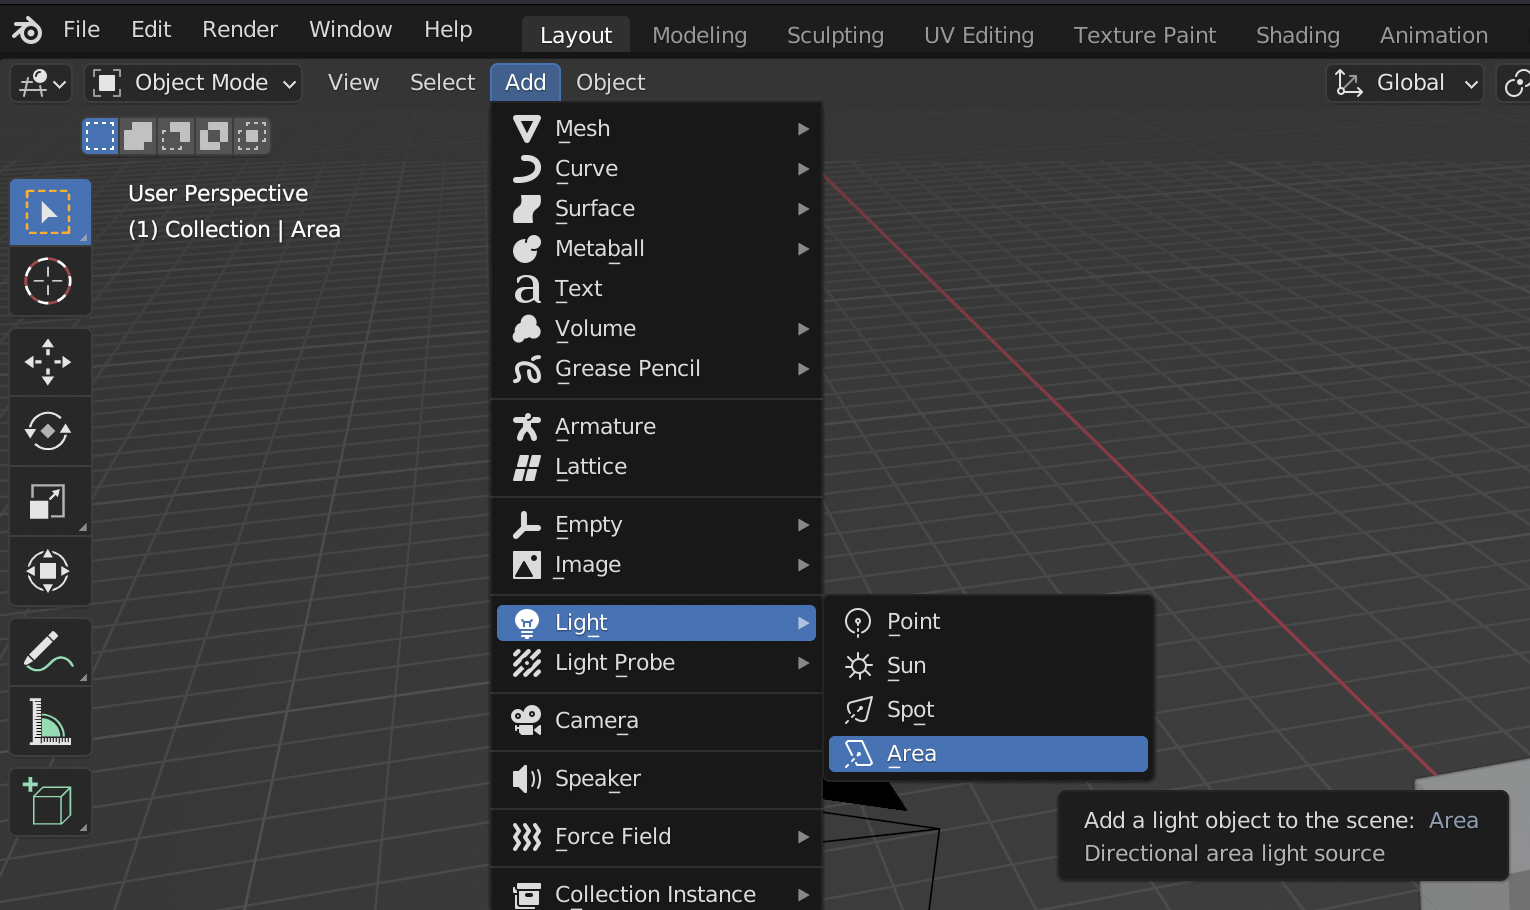
\includegraphics[width=4in]{images/adding-area-light.png}
    \caption{How to add an area light.}
\end{figure}

\subsubsection{The area lights method}
I rarely use this method, but I've listed it for completeness (I usually use Sun lights instead, described in Section~\ref{sec:TheSunLightMethod}.) 

I add a few area lights to illuminate the object from multiple sides. A quick way to add more lights is to duplicate an existing light (\keys{Shift + D}.) I fiddle with the angle and power of the lights, toggling the camera view and using the ``Rendered'' viewport shading to see how the object looks (FAQ~\ref{sec:FAQ-camera-view}), until I'm reasonably satisfied that the object is well-lit (Figure~\ref{fig:object-with-directional-lights}.) 
\begin{figure}[H]
    \centering
    \captionsetup{width=0.8\textwidth}
    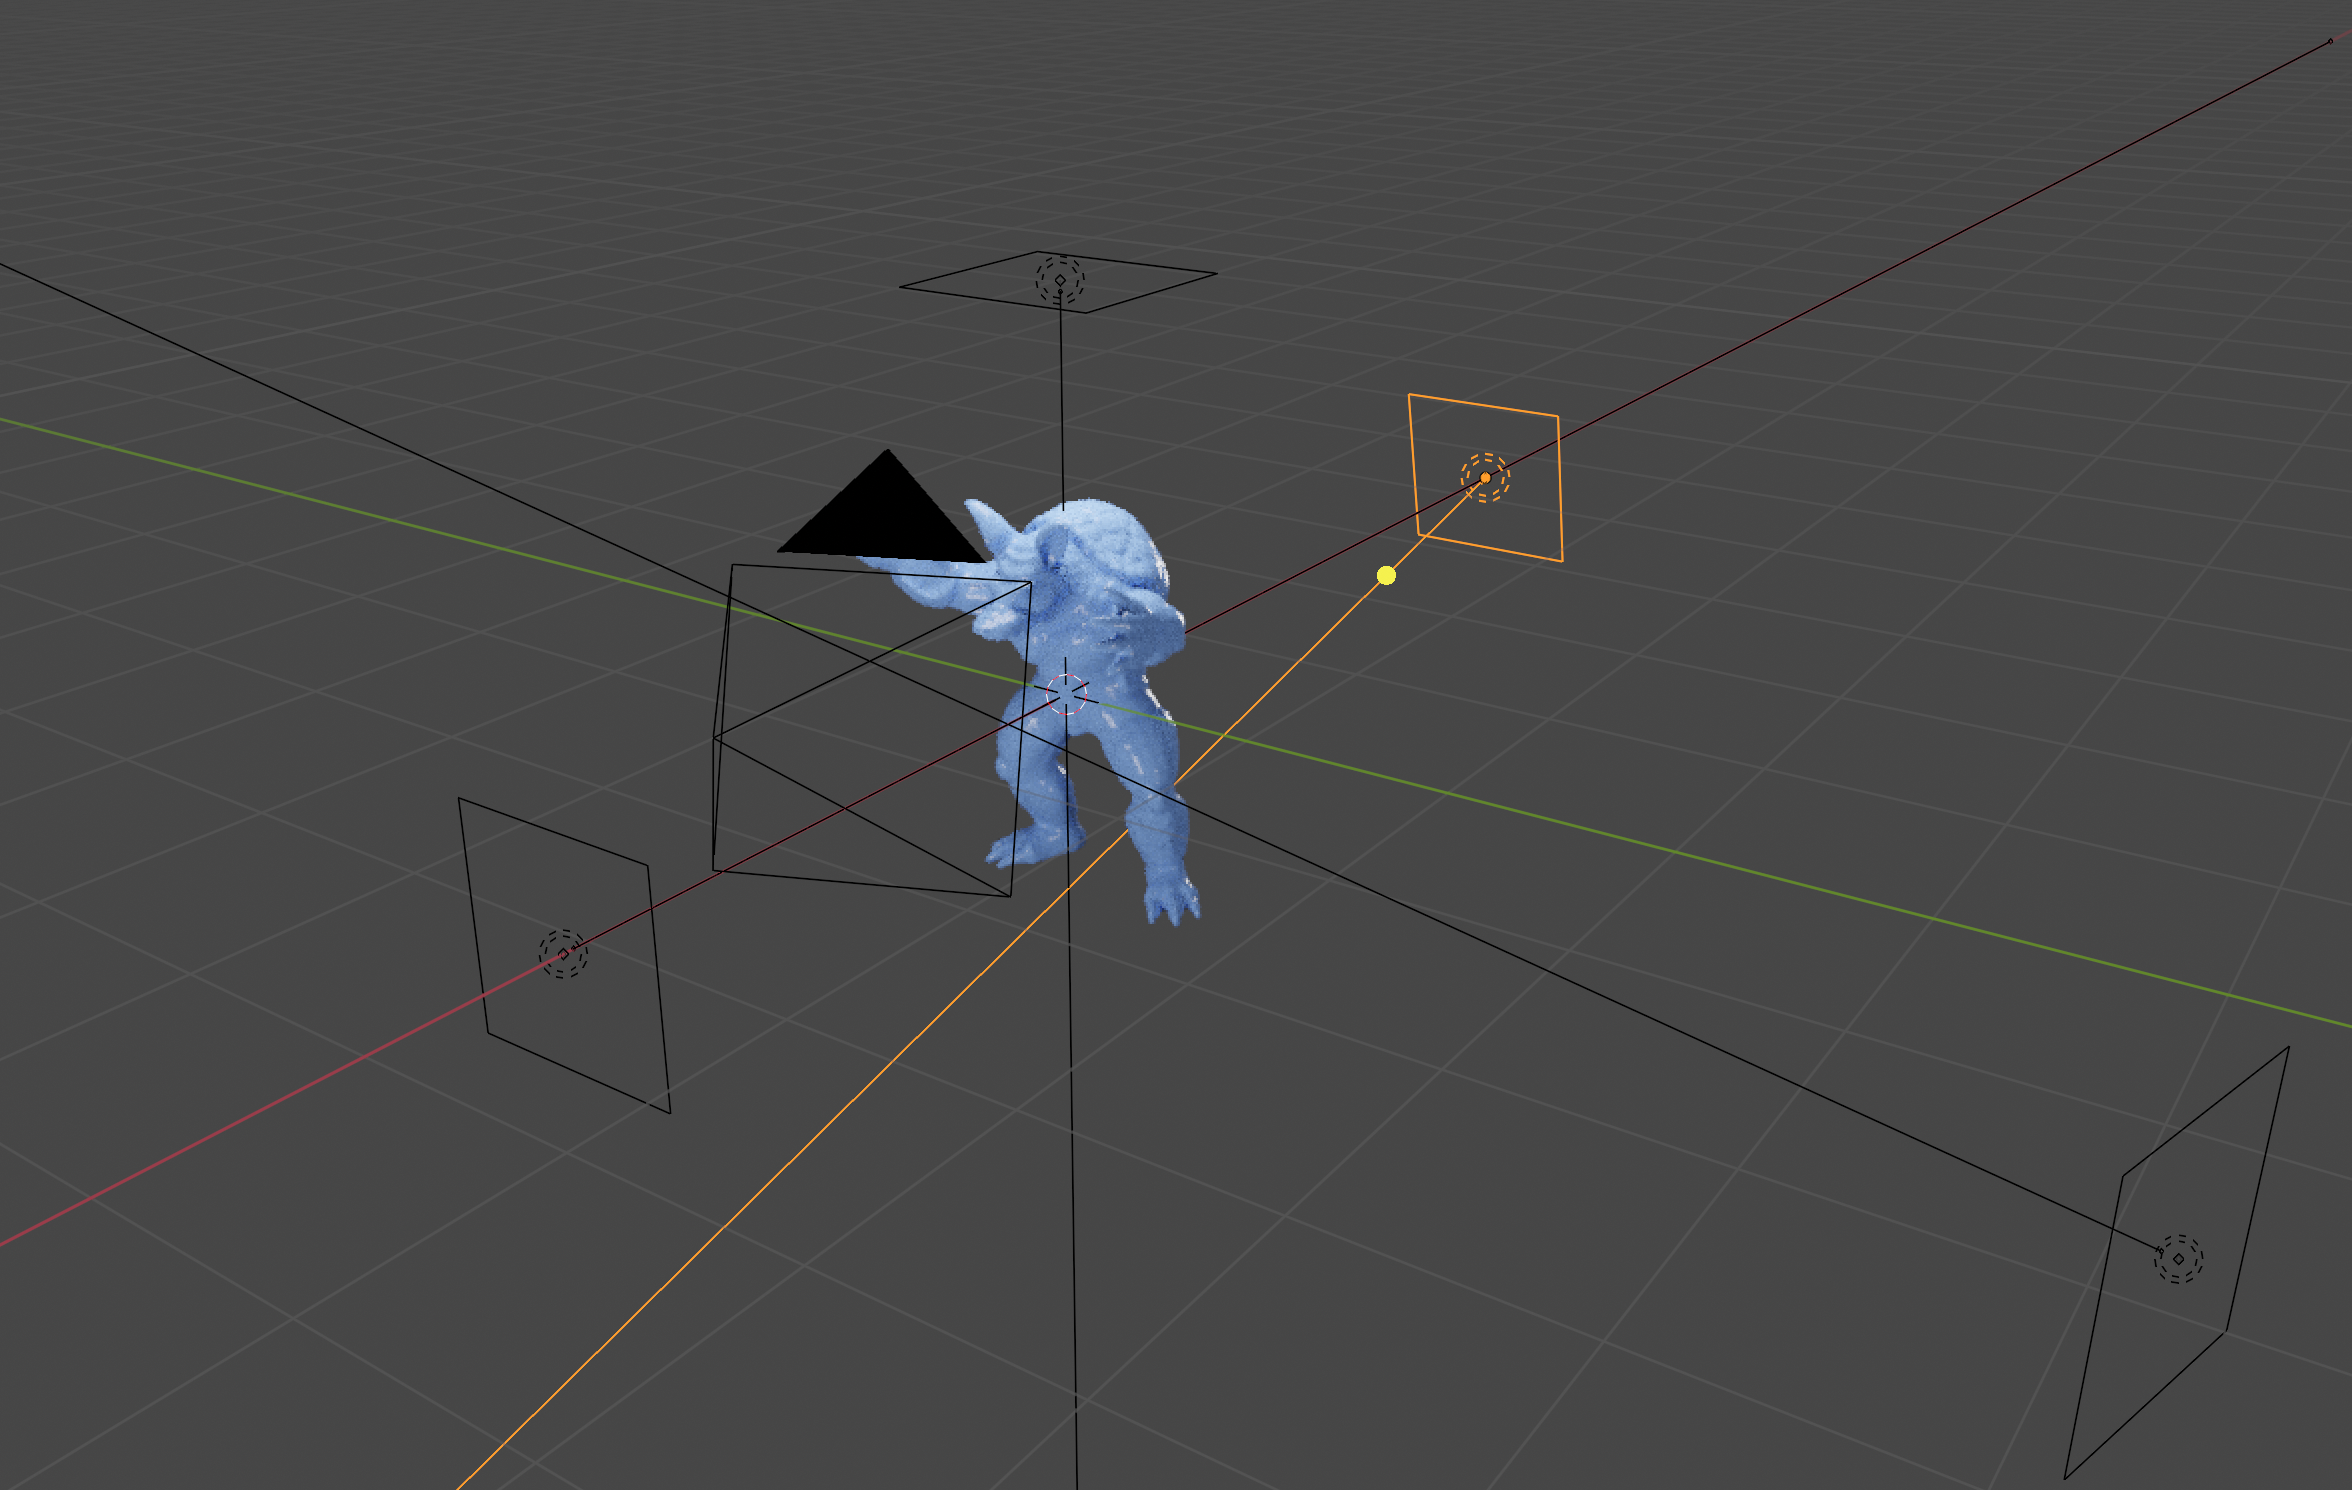
\includegraphics[width=5in]{images/object-with-directional-lights.png}
    \caption{An example of a scene with several directional lights added.}
    \label{fig:object-with-directional-lights}
\end{figure}

The power of the lights can be adjusted under \menu{Properties > Object Data Properties} (the \inlinepic{images/object-data-properties-light.png} icon in the right panel menu) -- see Figure~\ref{fig:area-light-settings}. The positioning and angles of the lights can be adjusted, just like any other object, under \menu{Properties > Object Properties} (\inlinepic{images/object-properties.png}.)

\begin{figure}[H]
    \centering
    \captionsetup{width=0.8\textwidth}
    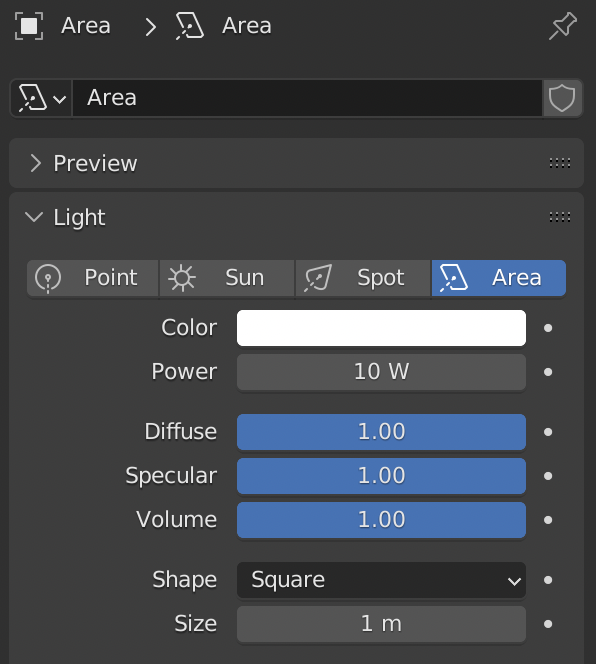
\includegraphics[width=2in]{images/area-light-settings.png}
    \caption{The light settings underneath \menu{Properties > Object Data Properties} (the \inlinepic{images/object-data-properties-light.png} icon.) Here, you can change the light's strength, or switch to a different type of light if needed. \label{fig:area-light-settings}}
\end{figure}

\subsubsection{The Sun light method}
\label{sec:TheSunLightMethod}
For typical single-object scenes, usually I only add one single ``Sun''-type light, which I usually find is enough to both illuminate the object sufficiently, and result in visually-pleasing shadows that are not too complicated. After adding a Sun light, I simply play with the X-, Y-, and Z-``Rotation'' parameters (by dragging the corresponding input boxes left and right) until the scene's objects have self-shadows that look good to me. For most of my scenes, I find that I usually have to increase the light's power $\sim$4000 watts (Figure~\ref{fig:area-light-settings}).

\begin{figure}[H]
    \centering
    \captionsetup{width=0.8\textwidth}
    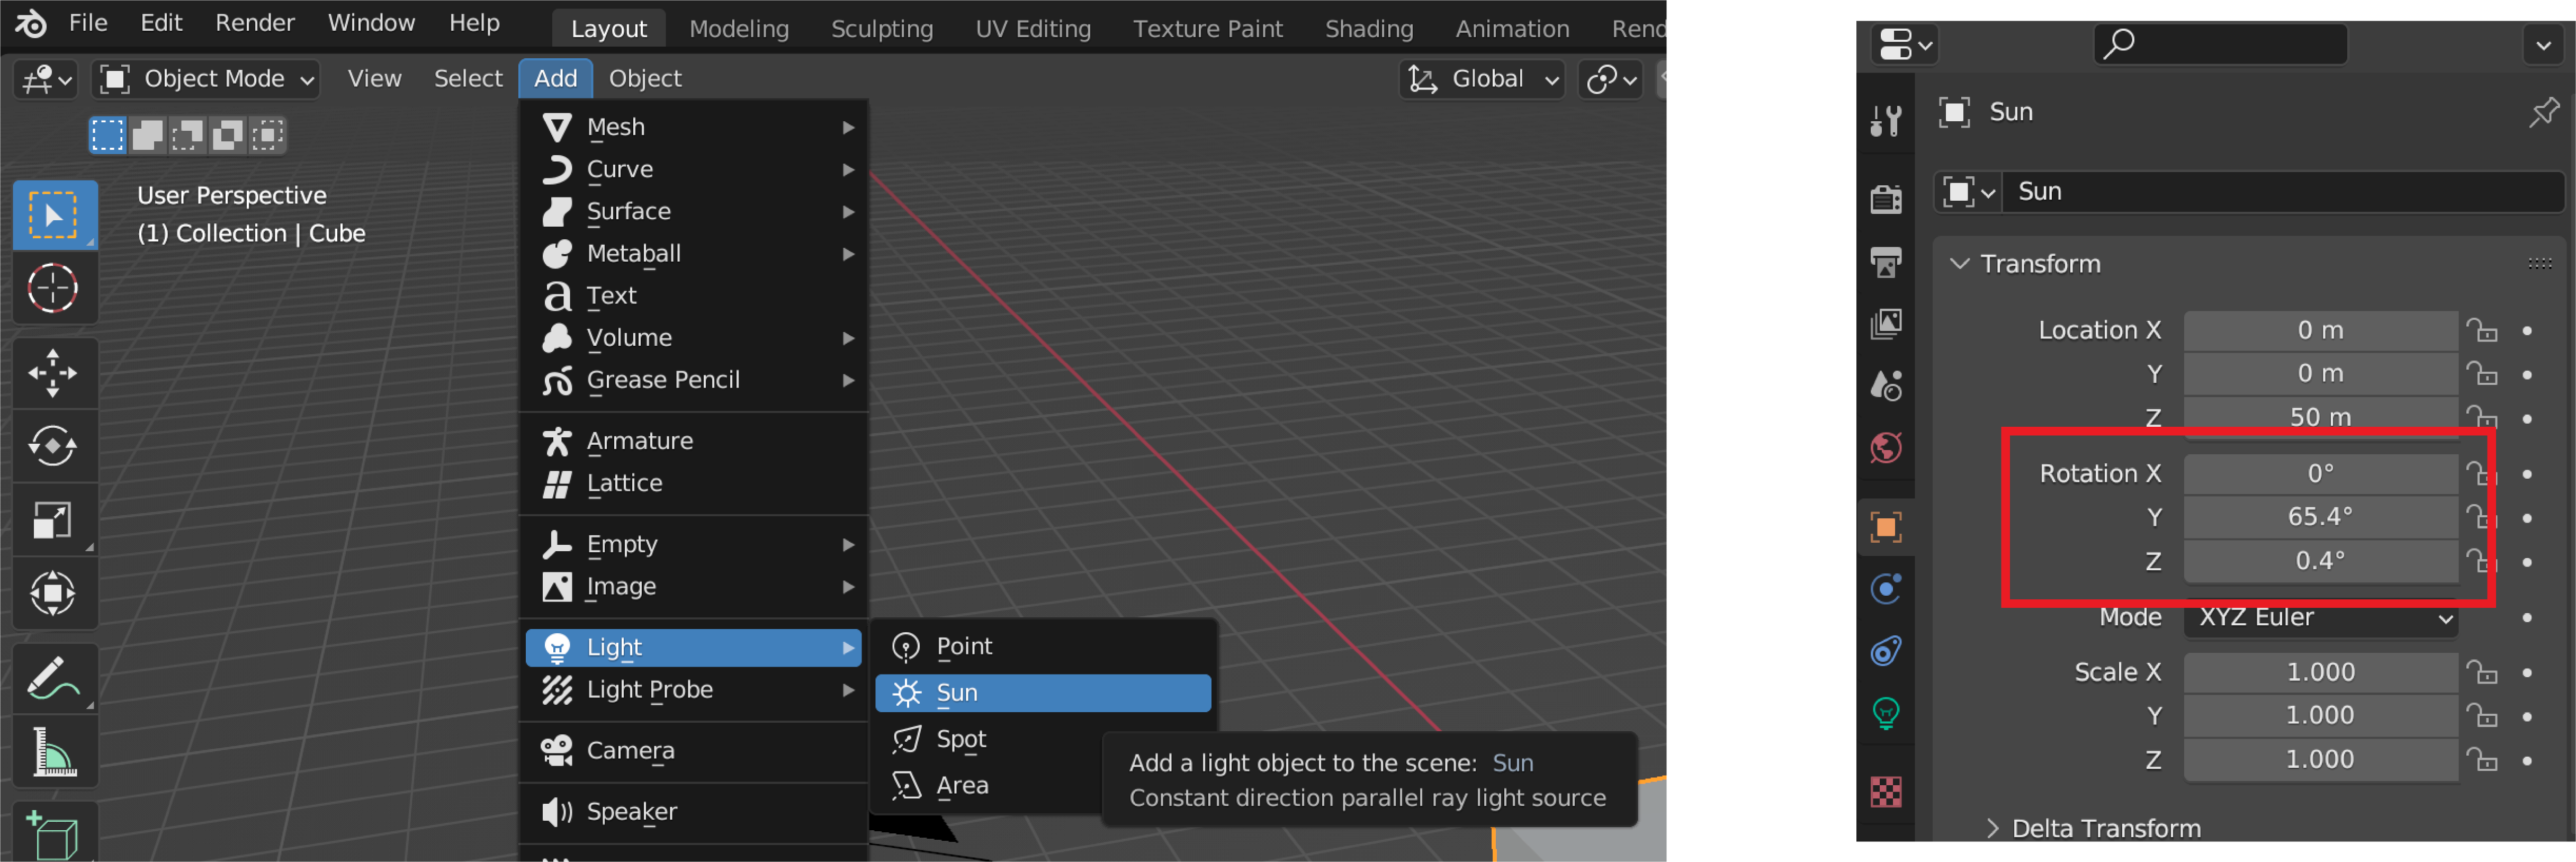
\includegraphics[width=6in]{images/SunLightRotations.png}
    \caption{\textit{Left:} Adding a Sun light. \textit{Right:} Under \menu{Properties > Object Properties} (the \inlinepic{images/object-properties-icon.png} icon), I simply play with the X-, Y-, and Z-``Rotation'' parameters (by dragging the corresponding input boxes left and right) until the scene's objects have self-shadows that look good to me. \label{fig:SunLightRotations}}
\end{figure}

\begin{figure}[H]
    \centering
    \captionsetup{width=0.8\textwidth}
    \includegraphics[width=3in]{images/DragonSunLit.png}
    \caption{An example of an object lit using a single Sun light --- the next section details the steps used to create the shadow. For more examples, see \href{}{this paper} where I lit every 3D scene with this method. \label{fig:BlockSunLit}}
\end{figure}


\section{Shadows}
\label{sec:Shadows}

\subsection{Cast shadows}

Rendered images are often lent a greater degree of ``realness'' and sense of 3D placement in the context of a paper when rendered with a cast shadow. This is usually done by adding an ``invisible'' plane onto which the shadow from the object is cast. To add a plane, go to \menu{Add > Mesh > Plane}.
\begin{figure}[H]
    \centering
    \captionsetup{width=0.8\textwidth}
    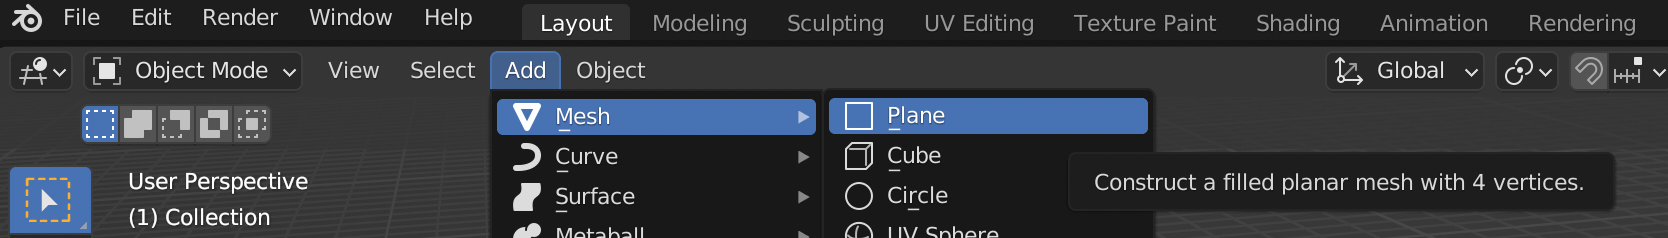
\includegraphics[width=4in]{images/add-a-plane-mesh.png}
    \caption{How to add a plane mesh.}
\end{figure}
Make the plane big enough so that it captures all of the object's shadow by scaling it under Object Properties (\inlinepic{images/object-properties-icon.png}.) Then apply the transforms by hitting \keys{Ctrl + A}.

To have the plane catch shadows but not actually be rendered in the final render, select the plane and turn on the ``Shadow Catcher'' option: Go to \menu{Properties > Object Data Properties > Visibility > Shadow Catcher}. You must be using the Cycles render engine, not Eevee, to use Shadow Catcher.
\begin{figure}[H]
    \centering
    \captionsetup{width=0.8\textwidth}
    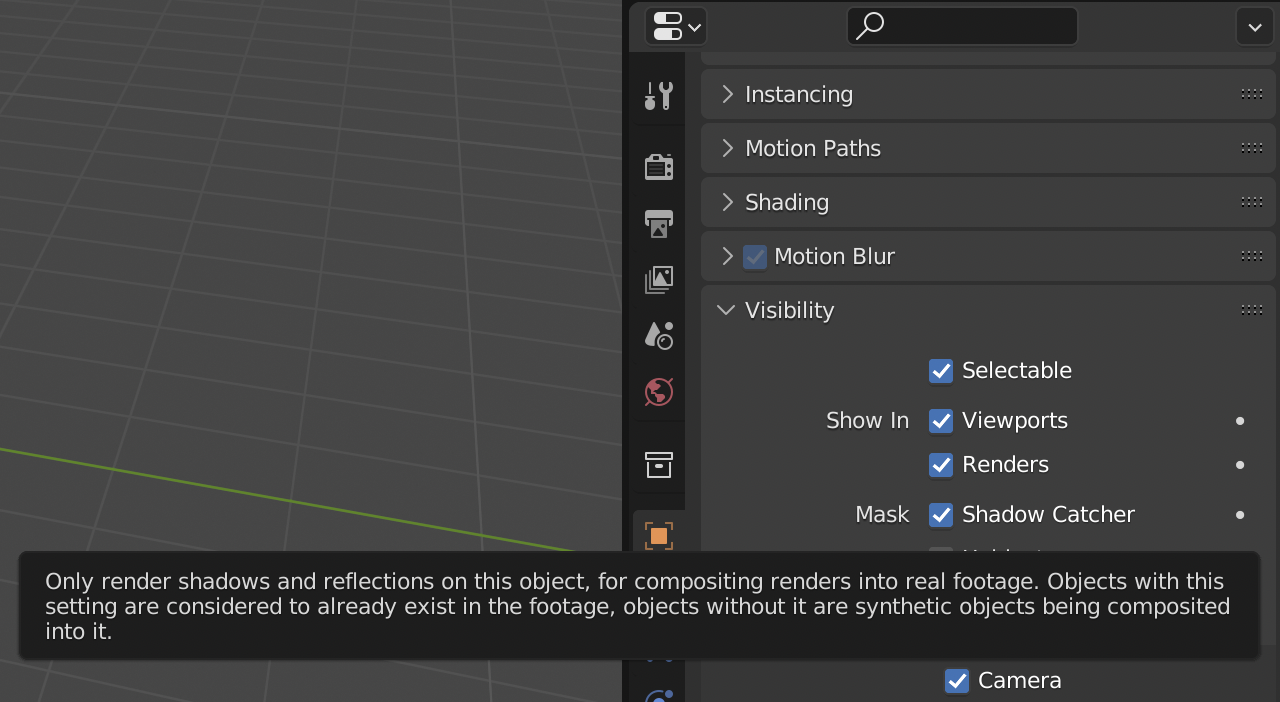
\includegraphics[width=4in]{images/shadow-catcher-option.png}
    \caption{Turning on the Shadow Catcher option. This option is often used for ground planes that are used to render shadows on an invisible ``ground''.}
    \label{fig:shadow-catcher-option}
\end{figure}

Usually, the light settings that best illuminate the scene objects well, such as those shown in Figure~\ref{fig:object-with-directional-lights}, are \textit{not} simultaneously ideal for generating clean-cut, well-positioned, aesthetically-pleasing cast shadows. I usually therefore create a second set of lights specifically for creating the shadow. To keep these lights logically separate from the original scene items, I add a new scene ``collection'' by right-clicking on ``Scene Collection'' in the \menu{Outliner} menu in the upper-right (Figure~\ref{fig:adding-a-new-collection}.)
\begin{figure}[H]
    \centering
    \captionsetup{width=0.8\textwidth}
    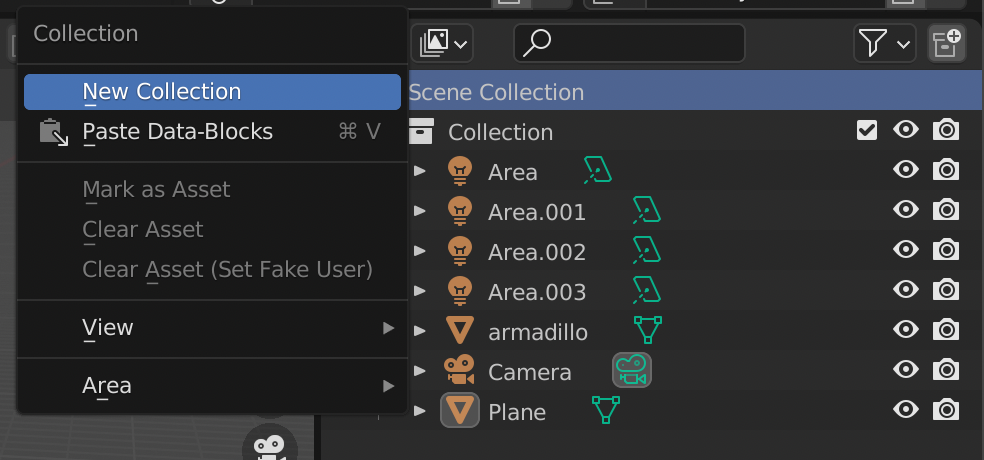
\includegraphics[width=4in]{images/adding-a-new-collection.png}
    \caption{Adding a new collection.}
    \label{fig:adding-a-new-collection}
\end{figure}
To this new collection, I add all the objects that are needed to make the shadow: the ground plane; a copy of the scene object(s), and additional light(s) that I've fiddled around with and deemed to make a good shadow. If the scene object(s) are particularly high-resolution and adding copies of them would slow the Blender and its rendering process down considerably, I just add lower-resolution versions of the objects (you don't need high-res objects to generate the shadows, which are fuzzy anyway!) Next, you want to select the ``Holdout'' option under \menu{Object Properties > Visibility}, which takes an object's occlusion into account in the render, without rendering the object itself:
\begin{figure}[H]
    \centering
    \captionsetup{width=0.8\textwidth}
    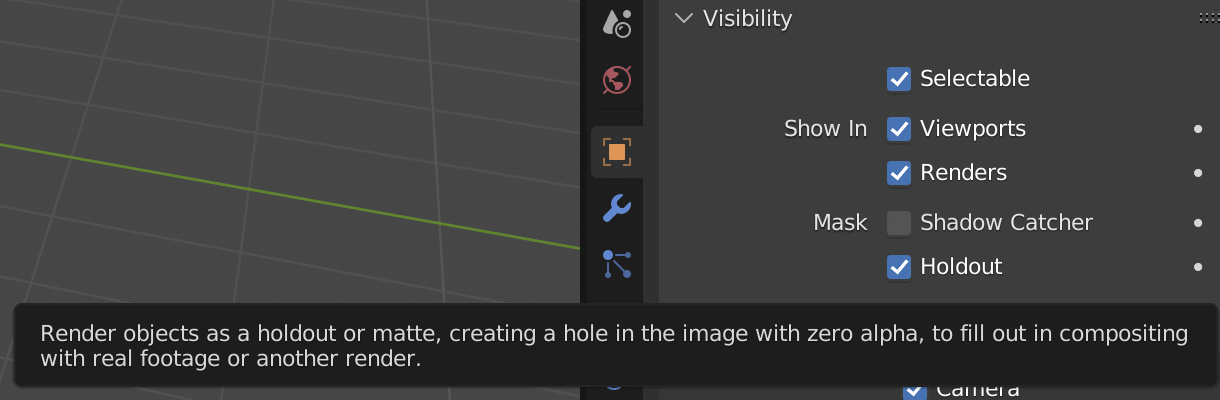
\includegraphics[width=4in]{images/holdout.png}
    \caption{Setting an object to rendered as ``holdout.''}
    \label{fig:holdout}
\end{figure}
For the light that generates the shadow, I usually add a ``Sun''-type light to make the shadow, as it tends to make the most clean-cut shadow whose positioning is easiest to control. I usually just place the sun somewhere above the scene objects; then fiddle around with its rotation under \menu{Object Properties > Rotation} (\inlinepic{images/object-properties-icon.png}) until the shadow looks okay to me in the viewport's render preview. Further, you can adjust the fuzziness of the shadow's outlines by increasing the ``Angle'' option in the light's \menu{Object Data Properties} (\inlinepic{images/object-data-properties-light.png}). An angle of $0^\circ$ will create a crisp shadow, while $2^\circ$ --- $4^\circ$ is usually enough to make a nice-looking ``fuzzy'' shadow. (I usually just use $0^\circ$.)
\begin{figure}[H]
    \centering
    \captionsetup{width=0.8\textwidth}
    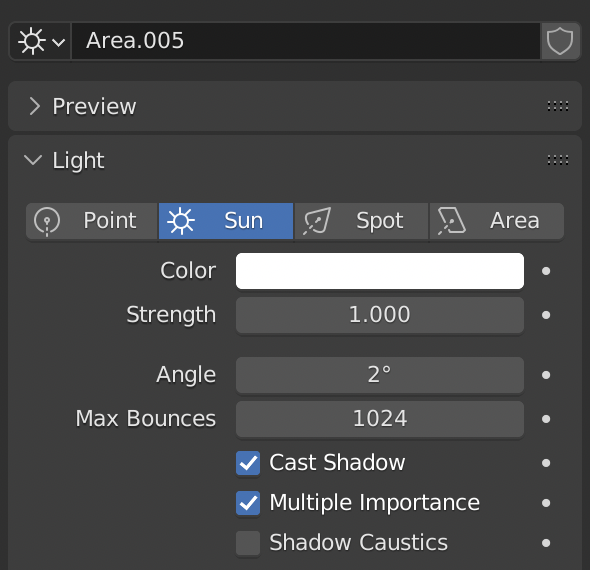
\includegraphics[width=3in]{images/sun-options.png}
    \caption{Adjusting the options of the ``Sun'' light to tune the resulting shadow. Increasing the angle will create a shadow with a fuzzier outline; I usually just use $0^\circ$. For most of my scenes, I usually increase the light's power $\sim$4000 watts, and set the ground plane's alpha value in the \menu{Shading} editor to 0.600, though I imagine these parameters will be somewhat scene-dependent.}
    \label{fig:sun-options}
\end{figure}
Sometimes the shadow is initially too dark. The easiest way to remedy this is to change the alpha value of the ground plane: Go to the \menu{Shading} editor, select the plane, and set its alpha value to something less than 1. For most of my scenes, I usually set the ground plane's alpha value 0.600.

We are now able to render two images separately: One containing just the lit and shaded object (no ground shadow, only self-shadows), and a second containing just the ground shadow. To render the two scene collections separately, toggle the camera icon next to the collection (``Disable in renders'', \inlinepic{images/disable-in-viewport-render.png}.) To avoid confusing myself, I always also toggle the ``Hide in viewport'' option as well (the eye icon) at the same time.
\begin{figure}[H]
    \centering
    \captionsetup{width=0.8\textwidth}
    \begin{subfigure}[b]{0.4\textwidth}
     \centering
     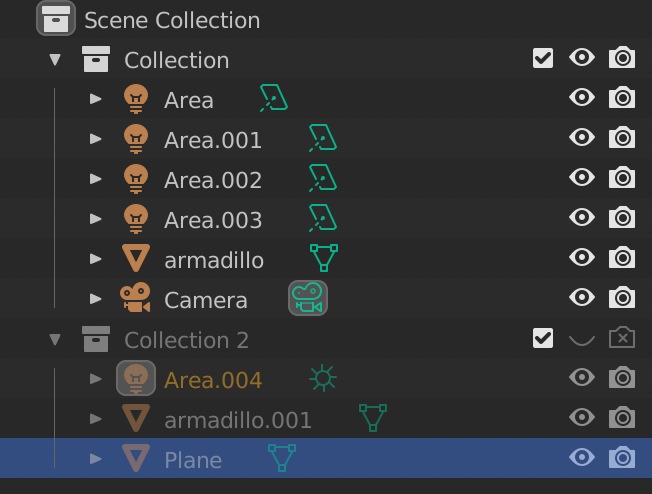
\includegraphics[width=0.9\textwidth]{images/collection-on-shadow-off.png}
     \caption{The lit and shaded objects will be rendered; the shadows are disabled.}
    \end{subfigure} \hspace{3mm}
    \begin{subfigure}[b]{0.4\textwidth}
     \centering
     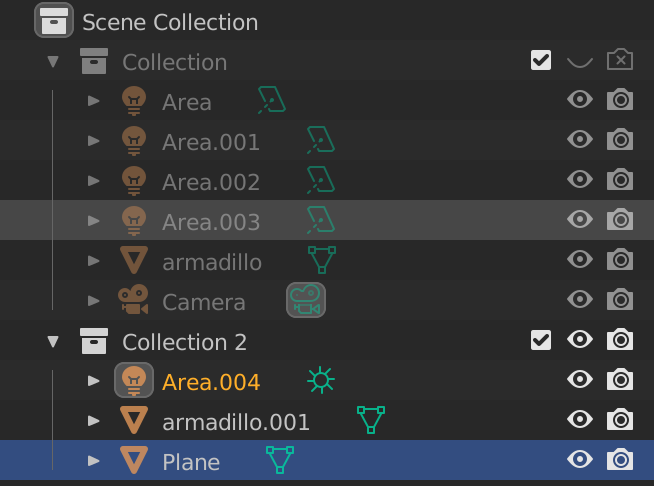
\includegraphics[width=0.9\textwidth]{images/collection-off-shadow-on.png}
     \caption{The lit and shaded objects are disabled from the render; the shadows will be rendered.}
    \end{subfigure}
    \caption{Rendering the scene objects separately from their shadows.}
    \label{fig:disable-in-render}
\end{figure}
After rendering these two images separately, I composite these two images together for the final figure (I use Adobe Illustrator.)
\begin{figure}[H]
    \centering
    \captionsetup{width=0.8\textwidth}
    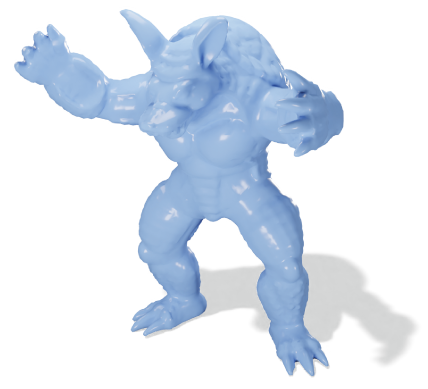
\includegraphics[width=3in]{images/final-render-with-shadow.png}
    \caption{A rendered object composited with its shadow. See also Figure~\ref{fig:DragonSunLit}.}
    \label{fig:final-render-with-shadow}
\end{figure}

\subsection{Non-physically-based shadows}
\label{sec:CartoonShadows}
Alternatively, you can add a ``shadow'' in a 2D graphics editor like Adobe Illustrator that only appears physically correct. Creating a shadow in this manner will be easier with regards to controlling the extent of the shadow, its shape, its crispness, etc. However, the shadow will almost inevitably have a more cartoonish/cel-shaded aesthetic to it. This might fit exactly into your aesthetic goals for the figure --- or it might make your render look fake and funny, so you should exercise your own judgement! % Sometimes physically-accurate shadows can be too complicated and distracting, and you desire a more streamlined figure that's a blend between realistically ray-traced \& a diagram/didactic feel.

\section{Function visualization}
\label{sec:FunctionVisualization}

\subsection{Setting colormaps}
You can either set the control points of a \obj{Color Ramp} node \href{https://blender.stackexchange.com/a/261366}{using a Python script} (which I personally find confusing), or use an image as a color map via a \obj{Image Texture} node (which I find much easier.) 

\href{https://matplotlib.org/stable/gallery/color/colormap_reference.html}{Matplotlib} has some examples of good color maps that are designed to be perceptually aligned with how the data might change. Many colormaps in Polyscope come from Matplotlib. Additionally, Mark has some \href{https://github.com/MarkGillespie/geoptic.js/blob/main/misc/generate_colormap_constant.py}{code} that samples from these colormaps and outputs a PNG; he has some examples \href{https://github.com/MarkGillespie/geoptic.js/tree/main/img/colormaps}{here}. 

Once you have the colormap image, simply add a \obj{Image Texture} node, select your image file, and hook the node up to the base color of your mesh (Figure~\ref{fig:color-map-texture}).
\begin{figure}[H]
    \centering
    \captionsetup{width=0.8\linewidth}
    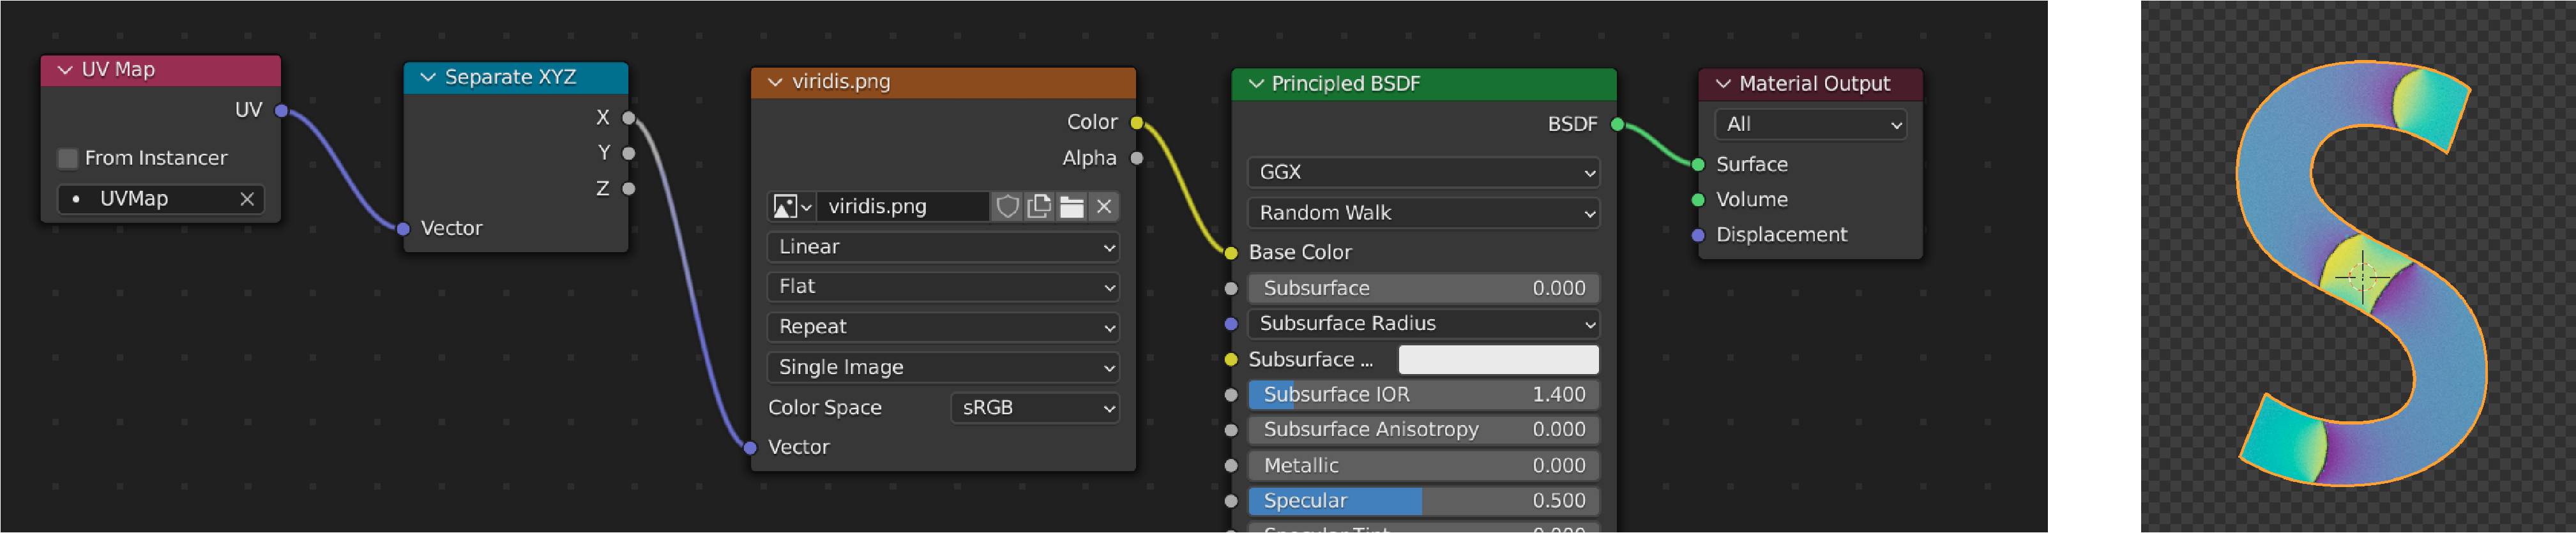
\includegraphics[width=0.9\linewidth]{images/color-map-texture.png}
    \caption{Using an external colormap to visualize scalar data. Left: The node configuration. Right: A viewport preview of the mesh, which is using the ``viridis'' colormap from Matplotlib.}
    \label{fig:color-map-texture}
\end{figure}

% Using nodes to scale/clamp values

{\bf Important:} Lights and materials will often interact with your colors in unexpected ways, leading to colors that are too washed out or too dark. This will look bad in a paper figure (Figure~\ref{fig:bad-color-management}), because your color bar legend will look like it's a different color than what's rendered on your surface:
\begin{figure}[H]
    \centering
    \captionsetup{width=0.8\textwidth}
    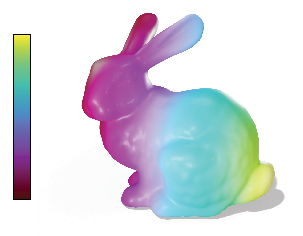
\includegraphics[width=4in]{images/bad-color-management.pdf}
    \caption{Bad color management! The texture-mapped colors look completely different than what they did originally.}
    \label{fig:bad-color-management}
\end{figure}

There are two main things you must do to get more accurate color-mapping. First is go to \menu{Properties > Render Properties > Color Management} (\inlinepic{images/2022-06-17_render-properties-icon.png}.) There is something in the Render Properties called the ``View Transform'' whose default is set to a non-standard option for some reason. You must switch to ``Standard'', which will then convert colors to the display the ``standard'' way. There are also contrast settings there (``Look'') although I find that leaving the default option to ``None'' is sufficient. 
\begin{figure}[H]
    \centering
    \captionsetup{width=0.8\textwidth}
    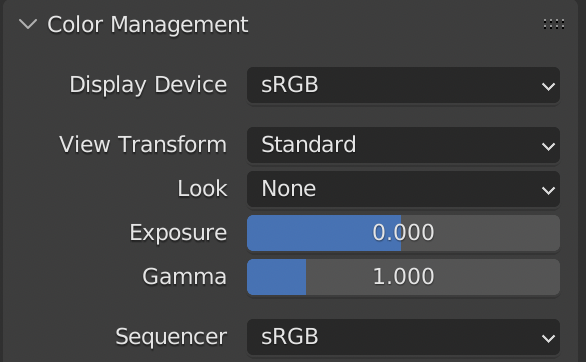
\includegraphics[width=3in]{images/color-management.png}
    \caption{The Color Management settings.}
    \label{fig:color-management}
\end{figure}
Further, to avoid the color of textures being washed out by the lights in your scene, you must add a separate ``Emission'' node in your shader. Hook up the output of the texture map to the input of \obj{Emission}. Add a \obj{Mix Shader} node to mix the output of \obj{Emission} with that of \obj{BSDF}. Pure emission would shade the object perfectly according to the colors in the texture, but would ignore the effects of the BSDF shader; to strike a good balance, leave the strength of \obj{Emission} at 1, and usually a value of 0.5 in \obj{Mix Shader} is good enough. After adding an emission shader, you may have to re-adjust some of the specular/roughness settings in \obj{BSDF} to retain the material appearance from before --- for this reason, I usually adjust emission settings before finalizing my material parameters.
\begin{figure}[H]
    \centering
    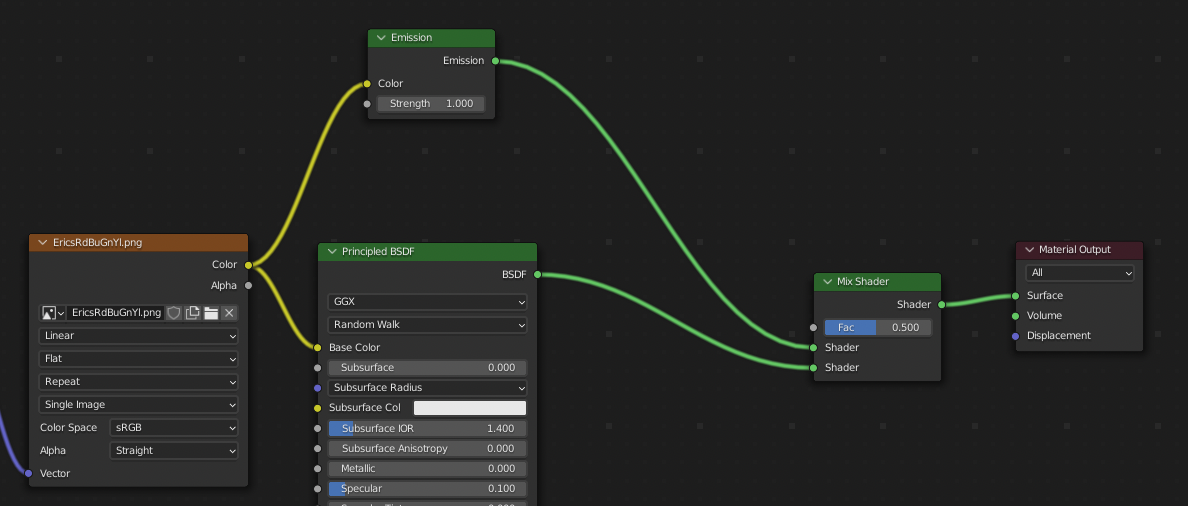
\includegraphics[width=5in]{images/emission-shader.png}
    \caption{Adding an emission shader.}
    \label{fig:emission-shader}
\end{figure}
Here is a better color-mapped surface:
\begin{figure}[H]
    \centering
    \captionsetup{width=0.8\textwidth}
    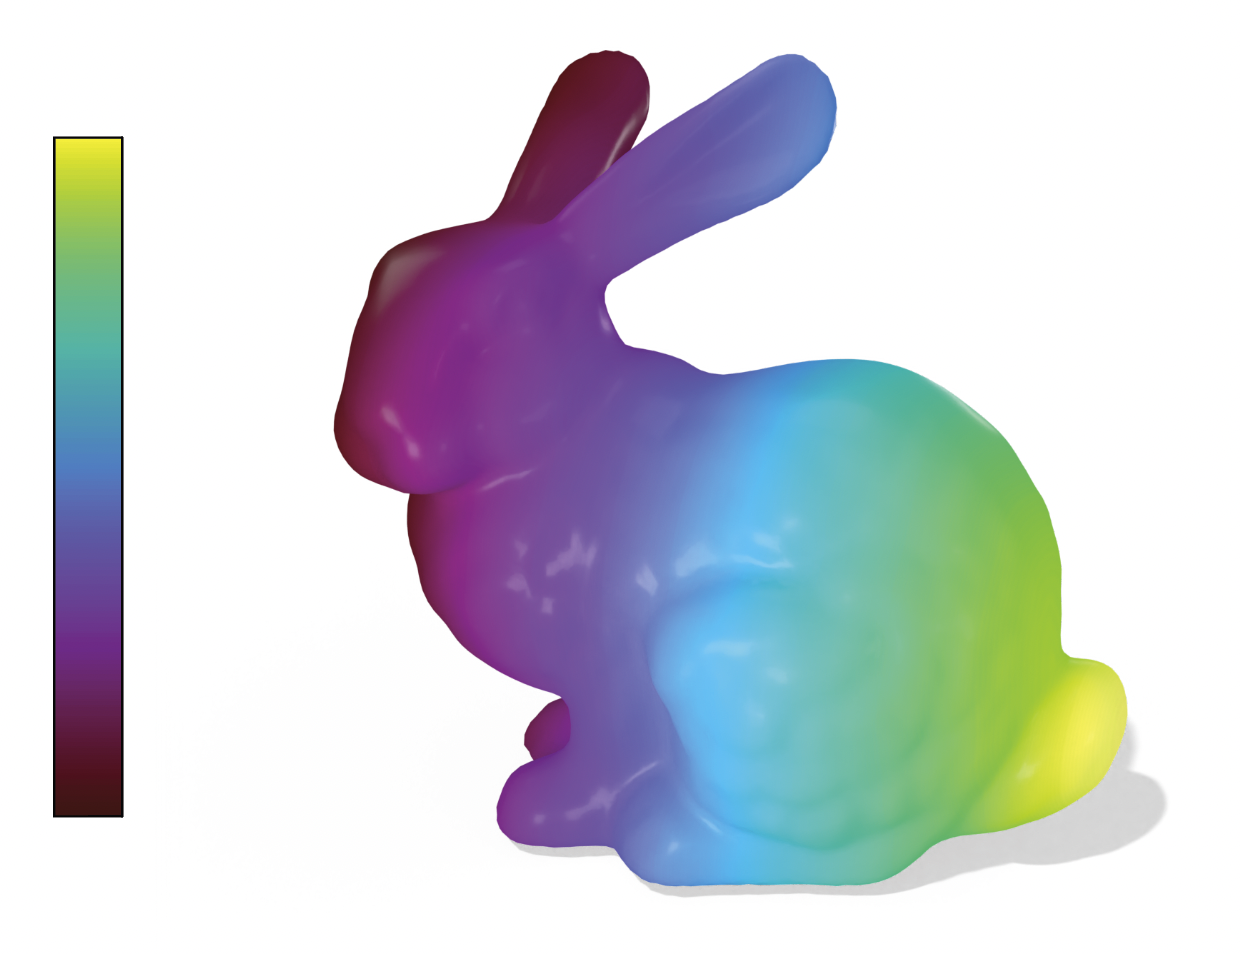
\includegraphics[width=4in]{images/better-color-management.png}
    \caption{Better color management --- the colors now match better between the colorbar and the texture-mapped color on the surface.}
\end{figure}

\subsection{Rendering isolines}
Sometimes you want to render a scalar function on a mesh, and also display its isolines. A classic example is a distance function.

\subsubsection{Using trigonometric functions}
To render isolines as darkened bands, I use the following method, which is based on tricks I picked up from looking at Inigo Quilez's shaders on \href{shadertoy.com}{Shadertoy}. (There are also simpler methods, described below.) Essentially, the scalar function $\phi$ is color-mapped as usual. But $\phi$ also gets mapped via a periodic function, which darkens the color quantity at regularly-spaced intervals (regularly-spaced numerically, that is. Whether the isolines actually end up being regularly-spaced spatially depends on whether $\phi$ is a true distance function.)

For the periodic function, a sinusoid is perfect the job; its range will eventually get mapped to $[0,1]$, representing the darkening factor. The sine function is especially nice because $\sin(0)=0$, which avoids having an isoband straddle the zero-set of the function. The period length controls the width of the isobands, and the amplitude controls the darkness. The function that computes the darkening factor is as follows:
% \begin{minted}[escapeinside=(**), mathescape=true]{c}
% // smoothstep() smooths out the bands, which avoids artifacts
% dark_factor((*$\phi$*)) = 1.0 - smoothstep(-a, a, (*$\sin(\omega\phi)$*))
% \end{minted}
\begin{center}
darkFactor($\phi$, $A$, $b$) = $A$ * smoothstep(-$b$, $b$, $\sin(\omega\phi)$)
\end{center}
This computes the factor by which the isobands are darkened. The amplitude $A$ controls the darkness of the isobands ($A\propto$ darkness), $\omega$ controls the width of the isobands ($\omega\propto \text{width}^{-1}$), and $b$ controls how much the function {\tt smoothstep()} smooths out the edges of the bands, which avoids artifacts ($b\propto$ smoothness.) 

Annoyingly, Blender doesn't have nodes that allow you to directly write your own script defining how to transform a quantity, like Houdini. Instead we build the darkening function by hooking up individual \obj{Math} nodes, which only allow for one atomic operation at a time. The smoothstep function is implemented in the \obj{Map Range} node; just select the ``Smooth step'' option. See Figure~\ref{fig:dark-isobands}.

The output of this chain of \obj{Math} nodes is a scalar between 0 and 1 that indicates the degree to which a color should be darkened. Hook the output of the last of the \obj{Math} nodes to the `{\tt Fac}' input of a \obj{Mix RGB} node, and hook the \obj{Color Ramp} output to the first `{\tt Color}' input of \obj{Mix RGB}. Set the second color of \obj{Mix RGB} to be black. This will allow us to blend between the original color map output, and a color that transitions to black, with the degree of transition controlled by the darkening factor we compute. The final node configuration is shown in Figure~\ref{fig:dark-isobands}.
\begin{figure}[H]
    \centering
    \captionsetup{width=0.8\textwidth}
    \begin{subfigure}[b]{0.9\textwidth}
     \centering
     \includegraphics[width=0.9\textwidth]{images/isoband-nodes.png}
     \caption{The node configuration.}
     \label{subfig:isoband-nodes}
    \end{subfigure} \\
    \begin{subfigure}[b]{0.9\textwidth}
     \centering
     \includegraphics[height=3in]{images/cat_isolines.png}
     \caption{The final render.}
     \label{subfig:isoband_final_render}
    \end{subfigure}
    \caption{Rendering isobands of a distance function on a kitty.}
    \label{fig:dark-isobands}
\end{figure}
Instead of blending with black, you can experiment with other colors or types of quantities (color, brightness, etc.) although I've found that simply blending with black or white yields best results.

A possible downside of this method is that it's not so straightforward to control the ratio of [width of dark bands]:[width of light bands]. You can kind of control the widths of the isobands by fiddling with the min/max values of the pre-image of smoothstep(), but this also affects the level of smoothness, so tends to result in overly-fuzzy bands. A better way to adjust the band width is to add another \obj{Map Range} node just before the \obj{Map Range} node that implements {\tt smoothstep()}. By re-mapping the output of $\sin$ from $[-1,1]$ to an interval that, for example, is mostly negative like $[-5,0]$, this forces the subsequent \obj{Map Range}, which is set up to map values onto $[0,1]$, to clamp all values less than its ``From minimum'' value to 0. Hence a narrower band of values receive darkening, resulting in thinner isobands. See Figure~\ref{fig:thin-isobands}.

\begin{figure}[H]
    \centering
    \captionsetup{width=0.8\textwidth}
    \begin{subfigure}[b]{0.9\textwidth}
     \centering
     \includegraphics[width=0.9\textwidth]{images/thin-isoband-nodes.png}
     \caption{Adding another \obj{Map Range} node (highlighted in white) to control the width of the isobands.}
     \label{subfig:thin_isoband-nodes}
    \end{subfigure} \\
    \begin{subfigure}[b]{0.9\textwidth}
     \centering
     \includegraphics[height=3in]{images/cat_thin_isolines.png}
     \caption{The final render.}
     \label{subfig:thin_isoband_final_render}
    \end{subfigure}
    \caption{Decreasing the isoband width and increasing the amplitude $A$ results in thin black lines.}
    \label{fig:thin-isobands}
\end{figure}

\subsubsection{Using modular arithmetic}
{\bf TODO:} Alternatively, you can also take mod 1 using a math node.

\section{Materials}
\label{sec:Materials}
For paper figures, I almost always just adjust the Specular, Roughness, and Clearcoat parameters of the \obj{Principal BSDF} node in the Shader until I'm happy with it.

\textbf{TODO:} PBR materials

\section{Additional visual effects}
\label{sec:Prettification}

\subsection{Adjust saturation/lightness}
{\bf TODO}

\subsection{Rim light effect}
\label{sec:RimLight}
This tip is courtesy of Mark, to get a ``glow'' effect around the silhouettes of the mesh. In photography and animation, rim lights / a rim light effect is used to increase contrast between the foreground object and background.

Enter the Shader editor (\Menu[t>]{Shading}.) 
\begin{enumerate}
    \item Add a \obj{Layer weight} node, and an \obj{Emission} node.
    \item Set the color of the emission to something lighter-colored, like white.
    \item Add a \obj{Mix Shader} node and drop it between \obj{Principled BSDF} and \obj{Material Output}. Hook up \obj{Emission} to the other ``Shader'' input of \obj{Mix Shader}. Finally, hook up the ``Fresnel'' output of \obj{Layer weight} to the ``Fac'' input of \obj{Mix Shader}, and set its value to something relatively small like 0.05.
\end{enumerate}
This method produces a white-ish glow around the silhouette of the mesh (Figure~\ref{fig:fresnel-glow}.) 

\begin{figure}[H]
    \centering
    \captionsetup{width=0.8\textwidth}
    \begin{subfigure}[b]{0.9\textwidth}
     \centering
     \includegraphics[width=0.7\textwidth]{images/2022-06-18_fresnel-glow-shading-nodes.png}
     \caption{The nodes.}
     \label{subfig:fresnel-glow-nodes}
    \end{subfigure} \\
    \begin{subfigure}[b]{0.45\textwidth}
     \centering
     \includegraphics[height=2in]{images/fresnel-glow-none.png}
     \caption{Without glow effect.}
     \label{subfig:fresnel-glow-none}
    \end{subfigure}
    \begin{subfigure}[b]{0.45\textwidth}
     \centering
     \includegraphics[height=2.3in]{images/fresnel-glow-effect.png}
     \caption{With glow effect.}
     \label{subfig:fresnel-glow}
    \end{subfigure}
    \caption{The glow effect (\ref{subfig:fresnel-glow}) can be more easily seen against a dark background. On the other hand, the glow around the outer silhouettes tends to be jagged.}
    \label{fig:fresnel-glow}
\end{figure}

\section{Common rendering settings}

\subsection{Rendering the final image}
To render the image, hit \keys{F12}. A separate render window will pop up.

\subsection{Smooth shading}
Most of the time we want our polygonal models to be smoothly shaded. In \Menu[t>]{Object} menu button in the upper left of the viewport (Figure~\ref{fig:shade_smooth}), click `Shade smooth' for smooth shading.
\begin{figure}[H]
    \centering
    \captionsetup{width=0.8\textwidth}
    \includegraphics[width=0.9\textwidth]{images/smooth-vs-flat-shading.png}
    \caption{The \menu{Object > Shade smooth} option (left.) The difference between `Shade flat' (middle) and `Shade smooth' (right) is shown (may need to zoom in to see the difference.)}
    \label{fig:shade_smooth}
\end{figure}
You can also use the \obj{Set Shade Smooth} node in \menu{Geometry Nodes}:
\begin{figure}[H]
    \centering
    \includegraphics[width=4in]{images/2022-09-07_set-shade-smooth.png}
    \caption{}
\end{figure}

\subsection{Eevee vs. Cycles}
\label{subsec:eevee_vs_cycles}
For better rendering quality, go to \menu{Properties > Render properties} (\inlinepic{images/2022-06-17_render-properties-icon.png} in the right panel menu.) For ``Render Engine'', select ``Cycles'' instead of ``Eevee''. ``Cycles'' uses ray-tracing.

On the other hand, rendering using ``Cycles'' takes a lot longer. While iterating on your scene, it may be wiser to use ``Eevee''; or at the very least, use ``Material Preview'' as your viewport shading, rather than ``Rendered'' (see Section~\ref{sec:viewport_shading}.)

When using ``Cycles'', typically a value of 50 for ``max samples'' during rendering is enough to produce a crisp picture. For more complicated geometry, transparency, etc. you may need more. You can also turn down the number of max samples to about 30 or so for viewport rendering.

\subsection{Rendering images with transparency}
To render images with transparent background, go to \menu{Properties > Render properties} (\inlinepic{images/2022-06-17_render-properties-icon.png} in the right panel menu.) Under the \directory{Film} drop-down menu, check the `Transparent'' box.

\subsection{View render with a transparent background against a white background}
\label{sec:preview_with_white_background}
It can be hard to tell if the lighting is correct in your scene just from the final render (which usually has a transparent background); you'll want to preview it against a white background, to see how the image will look in a paper document, slides, etc. You can do this either by pasting your rendered image into a separate document; or using the \menu{Compositing} editor with the following nodes:
\begin{figure}[H]
    \centering
    \captionsetup{width=0.8\textwidth}
    \includegraphics[width=6in]{images/2022-09-07_preview-in-compositor.png}
    \caption{Viewing a render with a transparent background against a white background in the Compositing editor.}
\end{figure}
{\bf TODO:} There's some weird gamma correction going on, so that the background isn't perfectly white --- I don't really use this method myself at the moment.

\section{Viewport options}

\subsection{Viewport shading}
\label{sec:viewport_shading}

In the upper right of the viewport, there are a few options for viewport shading. 
\begin{figure}[H]
    \centering
    \captionsetup{width=0.8\textwidth}
    \includegraphics[width=1in]{images/2022-09-07_viewport-shading-options.png}
    \caption{The viewport shading icons in the upper right of the viewport.}
\end{figure}
Usually ``Rendered'' is the most useful, since it is the closest to what your final render will look like. The ``Rendered'' shading can be slow/noisy if you're using Cycles however, so it may be more efficient to toggle ``Material Preview'' instead, or use Eevee.

\subsection{Changing viewport appearance}
% https://blender.stackexchange.com/questions/164502/how-to-change-the-viewport-background-color
% https://blender.stackexchange.com/questions/184721/how-do-you-change-the-background-color-of-the-3d-viewport/184728#184728

To change the default background color of the viewport, go to \menu{Edit > Preferences > Themes > 3D Viewport > Theme Space > Gradient Colors} and change the values of ``Gradient High/Low''. (The \Menu[t>]{Edit} menu is in the upper left of the main window.) This will change the default background color, i.e. the viewport background will now be this color every time you open a new Blender file. % To change the background color of just the current Blend file, go to \menu{Properties > Viewport Shading}.

You can also customize the vignetting in the viewport in \menu{Edit > Preferences > Themes > 3D Viewport > Gradient Colors > Background Type}.

\section{Scripting}
In theory, everything done using the Blender GUI can also be achieved via a Python script. Using a script is useful when you need to render many objects, and/or set similar rendering properties for each of them. You can look up documentation online about the \href{https://docs.blender.org/api/current/index.html}{Blender Python API}. Personally, I found it takes a definite effort to get the hang of scripting in Blender. It's helpful to start by trying to re-create a simple Blender example you have already done using the GUI -- for example, one of the examples in this document.

Also, Python scripting is essentially a programmatic way to manipulate the Blender GUI. Therefore, I expect it will be easier to learn to use Blender through the GUI first, before trying scripting. It's hard to know what to script without understanding how Blender expects objects to be manipulated.

A tip mentioned by ``Linus'' in the 2022 SGP Discord server: Enable \menu{Preferences > Interface > Python tooltips}, and then hovering over UI elements will tell you how to access it with Python.

Note: You must launch Blender from the command line to receive output to terminal.

\section{Useful keyboard shortcuts}

\subsection{Change view in viewport}
You can quickly snap to different views using \keys{1}, \keys{3}, \keys{7}, and \keys{9} on the numberpad. Each of them snaps to an axis-aligned view. Additionally, \keys{4} and \keys{6} rotate the view in increments around the z-axis; \keys{2} and \keys{8} incrementally rotate the view around the x-axis. Hitting \keys{5} toggles perspective vs. orthographic view.

Unfortunately these shortcuts only work on keyboards with a numberpad (unless you do some fancier keyboard re-mapping.)

\section{FAQs}
\subsection{How do I delete \underline{\hspace{1cm}}?}
Select the object and hit the \keys{x} key.

\subsection{How do I disconnect a node?}
There are a few ways to disconnect nodes:
\begin{enumerate}
    \item Hold down \keys{\ctrl} or \keys{\cmd}, and drag the right mouse button to ``cut'' links with a knife (see Figure~\ref{fig:disconnect_node}.)
    \begin{figure}[H]
        \centering
        \captionsetup{width=0.8\textwidth}
        \includegraphics[width=4in]{images/disconnect-node.png}
        \caption{Disconnecting nodes.}
        \label{fig:disconnect_node}
    \end{figure}
    \item Alternatively, hold down \keys{option}/\keys{alt} and use the left mouse button to drag a node ``out'' of a connection.
    \item Alternatively, you can simply grab the input connection with your mouse, and drag it off.
\end{enumerate}

\subsection{How do I preview the object before rendering?}
\label{sec:FAQ-camera-view}
Toggle the camera view (Figure~\ref{fig:toggle-camera-view}) to view the object in the viewport through the currently-active camera. Turn on the ``Rendered'' option under Viewport Shading (Figure~\ref{fig:rendered-viewport-shading}) to display in the viewport a preview of how your object will be lit and shaded.
\begin{figure}[H]
    \centering
    \includegraphics[width=3in]{images/toggle-camera-view.png}
    \caption{Toggling the camera view.}
    \label{fig:toggle-camera-view}
\end{figure}
\begin{figure}[H]
    \centering
    \includegraphics[width=4in]{images/rendered-viewport-shading.png}
    \caption{Turn on render preview in the viewport.}
    \label{fig:rendered-viewport-shading}
\end{figure}

\subsection{How do I use a different camera to render images, without affecting existing cameras?}


\section{Gotchas}

\subsection{Your scene probably needs a lot more light than you think}
\label{subsec:light_intensity}
Even if you set the background color of the viewport to white, objects will look brighter in Blender than they will on the white background of a paper. So you will have to add a lot more light than you think in order for the images to stand out on a white page. See Section~\ref{sec:preview_with_white_background} for how to view your (transparent background) image against a light-colored background.

% \subsection{Deleting highlighted text in the Blender text editor}
% You have to use the \keys{Delete} key to delete highlighted text in the text editor (Scripting editor); \keys{Backspace} won't work.
% \begin{figure}[H]
%     \centering
%     \includegraphics[width=0.5\textwidth]{images/2022-06-28_text-editor-deletion.png}
%     \caption{To delete the highlighted text, use \keys{Delete}.}
%     \label{fig:text-editor-deletion}
% \end{figure}
% It seems like as long as your click-and-drag while highlighting the text doesn't go outside the text editor, both \keys{Backspace} and \keys{Delete} work?

\subsection{Color management}
\label{sec:GotchaColorManagement}
Go to \menu{Properties > Render Properties > Color Management} and set ``View Transform'' to ``Standard'' to get non-washed out colors. To get accurate texture colors, see Section~\ref{sec:FunctionVisualization} for more detail.

\subsection{Receiving terminal output}
You must launch Blender from the command line to receive output to terminal, i.e. print statements and other useful error messages (helpful when debugging.) 

\part{Animations}

\end{document}